%!TEX program=xelatex
\documentclass[12pt]{report}

% -------------------------------------------------
% ЯЗЫК И ШРИФТЫ (XeLaTeX)
% -------------------------------------------------
\usepackage{fontspec}
\usepackage{polyglossia}
\usepackage{amsmath}
\usepackage{tikz}
\usetikzlibrary{patterns, arrows.meta}
\setdefaultlanguage{russian}
\setotherlanguage{english}
\setmainfont{Times New Roman}
\setsansfont{Arial}

\setmonofont{Menlo}

% -------------------------------------------------
% ГЕОМЕТРИЯ
% -------------------------------------------------
\usepackage[
  a4paper,
  left=25mm,
  right=20mm,
  top=20mm,
  bottom=25mm,
  headheight=16pt
]{geometry}

% -------------------------------------------------
% МАТЕМАТИКА
% -------------------------------------------------
\usepackage{amsmath,amssymb,amsfonts,mathtools}
\usepackage{mathrsfs}
\usepackage{bm}

% -------------------------------------------------
% ГРАФИКА И ТАБЛИЦЫ
% -------------------------------------------------
\usepackage{graphicx}
\usepackage{caption,subcaption}
\usepackage{booktabs,multirow,array,longtable,tabularx}
\usepackage{float}
\usepackage{tikz}
\usepackage{pgfplots}
\pgfplotsset{compat=1.18}

% -------------------------------------------------
% ТИПОГРАФИКА
% -------------------------------------------------
\usepackage{microtype}
\usepackage{indentfirst}
\usepackage{setspace}
\onehalfspacing
\setlength{\parindent}{1.25cm}
\setlength{\parskip}{0pt}
\usetikzlibrary{calc}
% -------------------------------------------------
% СПИСКИ
% -------------------------------------------------
\usepackage{enumitem}
\setlist{nosep}

% -------------------------------------------------
% ГИПЕРССЫЛКИ
% -------------------------------------------------
\usepackage[linktocpage=true]{hyperref}
\hypersetup{
  unicode=true,
  colorlinks=true,
  linkcolor=blue,
  citecolor=blue,
  urlcolor=blue,
  pdftitle={Конспект по математической физике},
  pdfauthor={Яков Овсянников},
  pdfauthor={Александр Лозовой}
}
\usepackage[nameinlink,noabbrev]{cleveref}
\usepackage{philex}
\bpaformat{1}{}{}
\renewcommand{\lbpa}[2]{%
  \refstepcounter{ExNo}%
  \noindent #2 \hfill (\theExNo)%
  \label{#1}%
  \par\medskip
}
\newcommand{\lbpn}[2]{%
  \refstepcounter{ExNo}%
  \noindent #2 \hfill (\theExNo)%
  \label{#1}%
  \par\medskip
}
% -------------------------------------------------
% КОЛОНТИТУЛЫ
% -------------------------------------------------
\usepackage{fancyhdr}
\pagestyle{fancy}
\fancyhf{}
\fancyhead[C]{\small Конспект по математической физике}
\fancyfoot[C]{\thepage}
\renewcommand{\headrulewidth}{0.4pt}
\renewcommand{\footrulewidth}{0pt}

\fancypagestyle{plain}{
  \fancyhf{}
  \fancyhead[C]{\small Конспект по математической физике}
  \fancyfoot[C]{\thepage}
  \renewcommand{\headrulewidth}{0.4pt}
}

% -------------------------------------------------
% ОФОРМЛЕНИЕ ГЛАВ
% -------------------------------------------------
\usepackage{titlesec}
\titleformat{\chapter}[display]
{\thispagestyle{plain}\normalfont\centering}
{\Huge\bfseries Глава \thechapter}
{0.8cm}
{\LARGE\bfseries}
[\vspace{0.8cm}]

\titleformat{\section}
{\normalfont\Large\bfseries}
{\thesection.}
{0.5em}
{}

\titleformat{\subsection}
{\normalfont\large\bfseries}
{\thesubsection.}
{0.5em}
{}

\titlespacing*{\chapter}{0pt}{0pt}{1cm}
\titlespacing*{\section}{0pt}{2ex}{1ex}

% -------------------------------------------------
% ОГЛАВЛЕНИЕ
% -------------------------------------------------
\usepackage{tocloft}
\renewcommand{\cfttoctitlefont}{\hfill\Large\bfseries}
\renewcommand{\cftaftertoctitle}{\hfill}
\renewcommand{\cftchapfont}{\bfseries}
\renewcommand{\cftchappagefont}{\bfseries}
\setlength{\cftbeforechapskip}{0.4em}

% -------------------------------------------------
% НУМЕРАЦИЯ
% -------------------------------------------------
\numberwithin{equation}{chapter}
\numberwithin{figure}{chapter}
\numberwithin{table}{chapter}

% -------------------------------------------------
% ПОДПИСИ
% -------------------------------------------------
\captionsetup{
  labelfont=bf,
  font=small,
  labelsep=period
}

% -------------------------------------------------
% ЦВЕТНЫЕ БЛОКИ
% -------------------------------------------------
\usepackage[most]{tcolorbox}

\definecolor{defback}{RGB}{235,245,255}
\definecolor{defframe}{RGB}{70,120,200}
\definecolor{exback}{RGB}{240,255,240}
\definecolor{exframe}{RGB}{70,150,90}
\definecolor{thmback}{RGB}{255,248,235}
\definecolor{thmframe}{RGB}{210,140,40}
\definecolor{lemmaback}{RGB}{250,245,255}
\definecolor{lemmaframe}{RGB}{130,90,180}
\definecolor{propback}{RGB}{245,250,255}
\definecolor{propframe}{RGB}{70,110,170}
\definecolor{remarkback}{RGB}{255,249,196}
\definecolor{remarkframe}{RGB}{212,175,55}
\definecolor{proofback}{RGB}{248,248,248}
\definecolor{proofframe}{RGB}{120,120,120}
\definecolor{exampleback}{RGB}{26, 240, 240}
\definecolor{exampleframe}{RGB}{161, 196, 196}
% -------------------------------------------------
% СЧЁТЧИКИ
% -------------------------------------------------
\newcounter{theoremctr}[chapter]
\renewcommand{\thetheoremctr}{\thechapter.\arabic{theoremctr}}

\newcounter{lemmactr}[chapter]
\renewcommand{\thelemmactr}{\thechapter.\arabic{lemmactr}}

\newcounter{propctr}[chapter]
\renewcommand{\thepropctr}{\thechapter.\arabic{propctr}}

\newcounter{remarkctr}[chapter]
\renewcommand{\theremarkctr}{\thechapter.\arabic{remarkctr}}

\newcounter{defctr}[chapter]
\renewcommand{\thedefctr}{\thechapter.\arabic{defctr}}

\newcounter{exectr}[chapter]
\renewcommand{\theexectr}{\thechapter.\arabic{exectr}}

\newcounter{examplectr}[chapter]
\renewcommand{\theexamplectr}{\thechapter.\arabic{examplectr}}
% -------------------------------------------------
% ИМЕНА ДЛЯ cleveref
% -------------------------------------------------
\crefname{theoremctr}{теорема}{теоремы}
\Crefname{theoremctr}{Теорема}{Теоремы}
\crefname{lemmactr}{лемма}{леммы}
\Crefname{lemmactr}{Лемма}{Леммы}
\crefname{propctr}{утверждение}{утверждения}
\Crefname{propctr}{Утверждение}{Утверждения}
\crefname{remarkctr}{замечание}{замечания}
\Crefname{remarkctr}{Замечание}{Замечания}
\crefname{defctr}{определение}{определения}
\Crefname{defctr}{Определение}{Определения}
\crefname{exectr}{упражнение}{упражнения}
\Crefname{exectr}{Упражнение}{Упражнения}
\crefname{examplectr}{пример}{примеры}
\Crefname{examplectr}{Пример}{Примеры}
% -------------------------------------------------
% ТЕОРЕМА
% -------------------------------------------------
\newtcolorbox{mytheorem}[1][]{
  enhanced,
  breakable,
  colback=thmback,
  colframe=thmframe,
  boxrule=0.9pt,
  arc=2mm,
  fonttitle=\bfseries,
  before=\refstepcounter{theoremctr},
  title={Теорема~\thetheoremctr},
  #1
}

% -------------------------------------------------
% ЛЕММА
% -------------------------------------------------
\newtcolorbox{mylemma}[1][]{
  enhanced,
  breakable,
  colback=lemmaback,
  colframe=lemmaframe,
  boxrule=0.9pt,
  arc=2mm,
  fonttitle=\bfseries,
  before=\refstepcounter{lemmactr},
  title={Лемма~\thelemmactr},
  #1
}

% -------------------------------------------------
% УТВЕРЖДЕНИЕ
% -------------------------------------------------
\newtcolorbox{myprop}[1][]{
  enhanced,
  breakable,
  colback=propback,
  colframe=propframe,
  boxrule=0.9pt,
  arc=2mm,
  fonttitle=\bfseries,
  before=\refstepcounter{propctr},
  title={Утверждение~\thepropctr},
  #1
}

% -------------------------------------------------
% ОПРЕДЕЛЕНИЕ
% -------------------------------------------------
\newtcolorbox{mydef}[1][]{
  enhanced,
  breakable,
  colback=defback,
  colframe=defframe,
  boxrule=0.8pt,
  arc=2mm,
  fonttitle=\bfseries,
  before=\refstepcounter{defctr},
  title={Определение~\thedefctr},
  #1
}

% -------------------------------------------------
% ДОКАЗАТЕЛЬСТВО
% -------------------------------------------------
\newtcolorbox{myproof}{
  enhanced,
  breakable,
  colback=proofback,
  colframe=proofframe,
  boxrule=0.8pt,
  arc=2mm,
  fonttitle=\bfseries,
  title={Доказательство}
}

% -------------------------------------------------
% УПРАЖНЕНИЕ
% -------------------------------------------------
\newtcolorbox{myexe}[1][]{
  enhanced,
  breakable,
  colback=exback,
  colframe=exframe,
  boxrule=0.8pt,
  arc=2mm,
  fonttitle=\bfseries,
  before=\refstepcounter{exectr},
  title={Упражнение~\theexectr},
  #1
}





% -------------------------------------------------
% ЗАМЕЧАНИЕ
% -------------------------------------------------
\newtcolorbox{myremark}[1][]{
  enhanced,
  breakable,
  colback=remarkback,
  colframe=remarkframe,
  boxrule=0.8pt,
  arc=2mm,
  fonttitle=\bfseries,
  before=\refstepcounter{remarkctr},
  title={Замечание~\theremarkctr},
  #1
}
% -------------------------------------------------
% Пример
% -------------------------------------------------

\newtcolorbox{myexample}[1][]{
  enhanced,
  breakable,
  colback=exampleback,
  colframe=exampleframe,
  boxrule=0.8pt,
  arc=2mm,
  fonttitle=\bfseries,
  before=\refstepcounter{examplectr},
  title={Пример~\theexamplectr},
  #1
}


% -------------------------------------------------
% ПОЛЕЗНЫЕ КОМАНДЫ
% -------------------------------------------------
% Множества
\newcommand{\R}{\mathbb{R}}
\newcommand{\N}{\mathbb{N}}
\newcommand{\Z}{\mathbb{Z}}
\newcommand{\Q}{\mathbb{Q}}
\newcommand{\C}{\mathbb{C}}
\newcommand{\E}{\mathbb{E}}
\newcommand{\D}{\mathcal{D}}
\newcommand{\B}{\mathcal{B}}
\newcommand{\F}{\mathcal{F}}
\newcommand{\LL}{\mathscr{L}}
\renewcommand{\L}{\mathcal{L}}
\newcommand{\circled}[1]{\tikz[baseline=(char.base)] \node[draw,circle,inner sep=1pt, minimum size=1.4em] (char) {#1};}
% Операторы
\newcommand{\sign}{\operatorname{sign}}
\renewcommand{\span}{\operatorname{span}}
\newcommand{\cl}{\operatorname{cl}}
\newcommand{\spec}{\operatorname{spec}}
\newcommand{\dom}{\operatorname{Dom}}
\newcommand{\Alt}{\operatorname{Alt}}
\newcommand{\supp}{\operatorname{supp}}
\newcommand{\arcsh}{\operatorname{arcsh}}
\newcommand{\arcch}{\operatorname{arcch}}
\newcommand{\arctanh}{\operatorname{arctanh}}
\newcommand{\arccth}{\operatorname{arccth}}

% Пространства
\newcommand{\DR}{\mathcal{D}(\R)}
\newcommand{\SR}{\mathcal{S}(\R)}
\newcommand{\SSR}{\mathcal{S}'(\R)}
\newcommand{\dR}{\mathcal{D}(\R^n)}
\newcommand{\ddR}{\mathcal{D}'(\R^n)}
\newcommand{\DDR}{\mathcal{D}'(\R)}
\newcommand{\Cinf}{\text{C}^{\infty}}

% Производные и интегралы
\newcommand{\p}{\partial}
\newcommand{\dd}{\mathop{}\!\mathrm{d}}
\newcommand{\ee}{\mathrm{e}}
\newcommand{\ii}{\mathrm{i}}
\newcommand{\grad}{\Vec{\nabla}}

% Скобки
\newcommand{\abs}[1]{\left|#1\right|}
\newcommand{\norm}[1]{\left\|#1\right\|}
\newcommand{\avg}[1]{\left\langle #1 \right\rangle}
\newcommand{\inner}[1]{\left\langle #1 \right\rangle}
\newcommand{\podst}[1]{\left[ #1 \right]}
\newcommand{\skobka}[1]{\left( #1 \right)}
\newcommand{\paren}[1]{\left(#1\right)}
\newcommand{\brackets}[1]{\left[#1\right]}
\newcommand{\set}[1]{\left\{#1\right\}}

% Специальные функции
\newcommand{\Pf}[1]{\mathrm{P}\dfrac{1}{#1}}
\newcommand{\PP}{\mathrm{P}\dfrac{1}{x}}
\newcommand{\px}[1]{\dfrac{1}{#1 \pm \mathrm{i}0}}
\newcommand{\Y}{\mathscr{Y}}
% Суммы и интегралы
\newcommand{\INT}{\int\limits_{-\infty}^{+\infty}}
\newcommand{\intpi}{\int\limits_{-\pi}^{+\pi}}
\newcommand{\sumn}{\sum_{n=0}^{\infty}}
\newcommand{\summ}{\sum_{m=0}^{\infty}}
\newcommand{\sumk}{\sum_{k=0}^{\infty}}
\newcommand{\SUMN}{\sum\limits_{n=1}^{\infty}}
\newcommand{\SUMM}{\sum\limits_{m=1}^{\infty}}
\newcommand{\SUMK}{\sum\limits_{k=1}^{\infty}}
\newcommand{\sumin}{\sum_{i=1}^{n}}
\newcommand{\sumkn}{\sum_{k=1}^{n}}
\newcommand{\SuM}{\sum\limits_{k=1}^{m}}
\newcommand{\disp}{\displaystyle}

% Оценки
\newcommand{\smallo}[2]{\underset{#1}{\overline{o}\left(#2\right)}}
\newcommand{\bigo}[2]{\mathop{O}\limits_{#1}\!\left(#2\right)}
\newcommand{\bigO}{\underline{O}}

% Разное
\newcommand{\vect}[1]{\mathbf{#1}}
\newcommand{\Let}{\sqsupset}
\newcommand{\ocup}{\overset{\circ}{\cup}}
\newcommand{\dopis}{\begin{center}\textbf{Дописать}\end{center}}
\newcommand{\ubf}[1]{\noindent\textbf{\underline{#1}}}
\newcommand{\theme}[1]{\noindent\textbf{\underline{#1}}\vskip2mm}
\newcommand{\RomanNumeralCaps}[1]{\MakeUppercase{\romannumeral #1}}
\newcounter{strcounter}
% Команда для нумерованной строки с меткой
\newcommand{\numberedline}[1]{%
  \refstepcounter{strcounter}%
  \makebox[0pt][r]{\thestrcounter\hspace{1em}}% номер справа с отступом
  \label{#1}%
}
% Переопределения греческих букв
\renewcommand{\phi}{\varphi}
\renewcommand{\epsilon}{\varepsilon}
\renewcommand{\kappa}{\varkappa}
% -------------------------------------------------
\setcounter{secnumdepth}{3}
\begin{document}


% =================================================
% ОБЛОЖКА
% =================================================
\begin{titlepage}
\thispagestyle{empty}
\centering

\vspace*{2.5cm}

{\Huge\bfseries Конспект по математической физике \par}
\vspace{0.8cm}

{\Large Весенний семестр 2026\par}

\vfill

{\large Лекторы\par}
\vspace{0.2cm}
{\Large Филонов Николай Дмитриевич\par}
{\Large Рядовкин Кирилл Сергеевич\par}

\vspace{0.8cm}

{\large \href{https://www.youtube.com/playlist?list=PLfpwmAe9eDRWlyIS1kNfHteBLl4A6B-Ce}
{Плейлист лекций}}
\vspace{0.2cm}
{\normalsize

\par}

\vspace{1.0cm}

{\large Над файлом работали\par}
\vspace{0.2cm}
{\normalsize
Яков Овсянников\par}
{\normalsize
Александр Лозовой\par}

\vspace{1.2cm}

{\large Университет ИТМО\par}

\end{titlepage}

% =================================================
% ОГЛАВЛЕНИЕ
% =================================================
\tableofcontents
\clearpage

% =================================================
% ГЛАВА 1
% =================================================
\chapter{Обобщенные функции}

\section{Определения}
\subsection{Класс основных обобщенных функций \texorpdfstring{$\DR$}{D(R)}}

\begin{mydef}
\[
\varphi \in \DR \Rightarrow
\begin{cases}
&\varphi \in C^{\infty}(\R),\\
&\supp \varphi \text{ - компакт, где } 
\supp \varphi = \overline{\{x: \varphi(x)\neq 0\}}
\end{cases}
\]
\end{mydef}

Рассмотрим типичный пример основной функции из $\DR$:
\[
\varphi(x)=
\begin{cases}
e^{\frac{1}{x^2-1}}, & |x|<1\\[0.5em]
0, & |x|\ge 1
\end{cases}
\]

Эта функция бесконечно дифференцируема на всей прямой и имеет компактный носитель, равный отрезку \( [-1,1] \).




\begin{figure}[H]
\centering
\begin{tikzpicture}
\begin{axis}[
    width=0.6\textwidth,
    height=0.45\textwidth,
    samples=400,
    axis lines=middle,
    axis line style={thick},
    xlabel={$x$},
    ylabel={$\varphi(x)$},
    xmin=-1.2, xmax=1.2,
    ymin=0, ymax=0.42,
    xtick={-1,-0.5,0,0.5,1},
    ytick={0,0.1,0.2,0.3,0.4},
    grid=both,
    major grid style={gray!30},
    minor grid style={gray!15},
    tick style={black,thick},
    label style={font=\small}
]

\addplot[
    very thick,
    blue,
    smooth,
    domain=-0.999:0.999
]
{exp(1/(x^2-1))};

\addplot[thick, black] coordinates {(-1.2,0) (-1,0)};
\addplot[thick, black] coordinates {(1,0) (1.2,0)};

\end{axis}
\end{tikzpicture}
\caption{График функции \(\varphi(x)\)}
\end{figure}


\begin{myexe}
    Доказать что $\varphi(x)\in \DR$. \\
$\supp\phi={x: |x|<1}$, его замыкание даёт [-1; 1], что является компактным множеством. $\dfrac{1}{x^2-1}$ - гладкая на (-1, 1), поэтмоу экспонента тоже гладкая, значит $\in\Cinf(\R)$.

\end{myexe}
Тогда ясно, что $\DR$ -- линейное пространство

\begin{mydef}
    \lbpn{zeroo}{\[\varphi_k \xrightarrow{\DR} \varphi \Leftrightarrow \,\begin{aligned}
&\exists A,B: \supp{\varphi_k},\supp{\varphi\subset [A,B]}\\
&\varphi_k^{{(m)}}\xrightarrow{k\rightarrow \infty} \varphi^{{(m)}} \,\text{равномерно на} \,[A,B] \,\text{для} \,\forall m
\end{aligned}\]}
\end{mydef}

\begin{myexe}
    Показать что $\DR$ -- не метризуемо, т.е. $\nexists \rho$ -- метрики: $\rho(\varphi_k,\varphi) \rightarrow0 \Leftrightarrow \varphi_k \xrightarrow{\DR} \varphi$
\begin{figure}[H]
        \centering
        
\includegraphics[width=0.6\linewidth]{pics/0.png}
        \caption{}
        \label{fig:enter-label}
\end{figure}
\end{myexe}


\subsection{Класс обобщенных функций \texorpdfstring{$\DDR$}{ }}

\begin{mydef}
    \[f\in\DDR \Leftrightarrow f -- \text{линейный непрерывный функционал на }\, \DR\]
    \[f:\DR \rightarrow \mathbb{C}\]
\end{mydef}
Другими словами \[\varphi\rightarrow(f, \varphi)\]
Посмотрим на линейность и непрерывность.
\\ 
\textbf{1) } Линейность: \\
$(f,\lambda\varphi+\mu\psi)=\lambda(f,\varphi)+\mu(f,\psi)$ для $\forall \lambda,\mu\in\mathbb{C}$ и $\varphi,\psi \in \DR$\\
\textbf{2) } Непрерывность:\\ Если $\varphi_k \xrightarrow{\DR} \varphi$, то $(f,\varphi_k)\rightarrow(f,\varphi)$


\begin{myremark}
    1) distribution\\
    2) непрерывность достаточно проверять только в нуле\\
    3) Если $f$- непрерывна и $\varphi_k\rightarrow0$, то $(f,\varphi_k)\rightarrow0$\\
    4) Если $f$ -- линейный функционал и $\varphi_k\rightarrow0,$ то $(f,\varphi_k)\rightarrow0$\\
    5) Пусть $\psi_k\xrightarrow{\DR} \psi$, тогда $(f,\psi_k)=(f,\psi_k-\psi)+(f,\psi)\rightarrow(f,\psi)$
\end{myremark}
Примеры таких функционалов:
\begin{enumerate}
\item 
\[
(\delta,\varphi)=\varphi(0)
\]

Если $\varphi_k \to \varphi$, то
\[
\varphi_k(0) \to \varphi(0).
\]
\item \label{2}\[
\left(\PP,\varphi\right)=
\operatorname{v.p.}\int\limits_{\R}\dfrac{\varphi(x)\dd x}{x}
=
\lim_{\varepsilon \to +0}
\int\limits_{|x|>\varepsilon} \dfrac{\varphi(x)}{x}\,\dd x
\] Предположим, что $\supp \subset[-R,R]$, тогда наш интеграл можно разбить на два:
\[=\lim_{\varepsilon \to +0}\left(\int\limits_{-R}^{-\varepsilon}+\int\limits_{\varepsilon}^{R}\right)\dfrac{\varphi(x)}{x}\,\dd x = 
\lim_{\varepsilon \to +0}\left(\int\limits_{-R}^{-\varepsilon}+\int\limits_{\varepsilon}^{R}\right)\dfrac{\varphi(x)-\varphi(0)}{x}\,\dd x=\int\limits_{-R}^{R}\dfrac{\varphi(x)-\varphi(0)}{x}\,\dd x\]
Линейность этого факта достаточно очевидна, поэтому посмотрим на \textit{непрерывность}.
\[\varphi_k \xrightarrow{\DR}0  \quad \text{и}\quad \supp \varphi_k\subset[-R,R]\]
Тогда получим следующую цепочку равенств:
\[\left|(\PP,\varphi_k)\right|=\left|\int\limits_{-R}^{R}\dfrac{\varphi_k(x)-\varphi_k(0)}{x}\,\dd x \right|\leq 2R\cdot \max_{x \in [-R,R]}|\varphi_k'|\xrightarrow{k\to\infty}0\]

\item  \[\left(\px{x},\varphi\right)=\lim_{\varepsilon\to+0}
\int\limits_{\R}
\dfrac{\varphi(x)}{x\pm \ii \varepsilon}\,\dd x\]



Пусть $\varphi \in \DR$. Тогда существует $R>0$ такое, что
\[
\supp \varphi \subset [-R,R]
\]
Следовательно:
\[
\int\limits_{\R}
\dfrac{\varphi(x)}{x\pm \ii \varepsilon}\,\dd x
=
\int\limits_{-R}^{R}
\dfrac{\varphi(x)}{x\pm \ii \varepsilon}\,\dd x =
\int\limits_{-R}^{R}
\dfrac{x\,\varphi(x)}{x^2+\varepsilon^2}\,\dd x
\mp
\ii
\int\limits_{-R}^{R}
\dfrac{\varepsilon\,\varphi(x)}{x^2+\varepsilon^2}\,\dd x 
\]

Первый интеграл в точности совпал с выражением \eqref{2}, поэтому исследуем второй:

\[
\int\limits_{-R}^{R}
\dfrac{\varepsilon\,\varphi(x)}{x^2+\varepsilon^2}\,\dd x
=
\int\limits_{-R}^{R}
\dfrac{\varepsilon(\varphi(x)-\varphi(0))}{x^2+\varepsilon^2}\,\dd x
+
\varphi(0)\int\limits_{-R}^{R}
\dfrac{\varepsilon}{x^2+\varepsilon^2}\,\dd x
\]
Первый интеграл стремится к нулю при $\varepsilon\to +0$. Для второго имеем
\[
\int\limits_{-R}^{R}\dfrac{\varepsilon}{x^2+\varepsilon^2}\,\dd x
=
\int\limits_{-R/\varepsilon}^{R/\varepsilon}\dfrac{1}{1+t^2}\,\dd t
\to
\int\limits_{-\infty}^{\infty}\dfrac{1}{1+t^2}\,\dd t
=
\pi 
\]
Следовательно:
\[
\int\limits_{-R}^{R}
\dfrac{\varepsilon\,\varphi(x)}{x^2+\varepsilon^2}\,\dd x
\to
\pi\,\varphi(0)
\]
То есть
\[
\lim_{\varepsilon\to+0}
\int\limits_{-R}^{R}
\dfrac{\varphi(x)}{x\pm \ii \varepsilon}\,\dd x
=
\left(\Pf{x},\varphi\right)
\mp
\ii \pi \varphi(0)
\]
Так как
\[
(\delta,\varphi)=\varphi(0),
\]
получаем
\[
\left(\dfrac{1}{x\pm \ii 0},\varphi\right)
=
\left(\Pf{x},\varphi\right)
\mp
\ii\pi(\delta,\varphi)
\]
\end{enumerate}
\begin{myprop}
Для любой функции $\varphi \in \DR$ существует предел:
\[
\left(\dfrac{1}{x\pm \ii 0},\varphi\right)
\coloneqq
\lim_{\varepsilon \to +0}
\int\limits_{-\infty}^{\infty}
\dfrac{\varphi(x)}{x\pm \ii \varepsilon}\,\dd x 
\]
Формула Сохоцкого выглядит следующим образом:
\[
\dfrac{1}{x\pm \ii 0}
=
\Pf{x}\mp \ii \pi \delta(x)
\]
\end{myprop}


\subsection{Регулярные и сингулярные обобщенные функции}
\lbpa{zero}{$f\in L_{1,loc}$ -- измеримая по Лебегу функция. $\int\limits_{a}^{b}\left|f(x)\right| \dd x< \infty$.} Тогда $\Tilde{f}$ -- функционал такой что:
\[(\Tilde{f},\varphi)=\int\limits_{\R}f(x)\varphi(x)\dd x \, - \text{линейный функционал на }\DR\Rightarrow \supp{\varphi_k} \subset [-R,R]\]
\[\varphi_k\xrightarrow{\DR}0\Rightarrow|(\Tilde{f},\varphi)|\leq \int\limits_{-R}^{R}f(x)|\varphi_k(x)|\dd x\leq \int\limits_{-R}^{R}|f(x)|\max_{x \in [-R,R]}|\varphi_k'|\rightarrow0\]
Видно, что функция непрерывна в нуле $\Rightarrow$ непрерывна везде $\Rightarrow \Tilde{f}\in \DDR$ 

\begin{mydef}
    $\Tilde{f}$-- \textit{регулярные} обобщенные функции, все остальные -- \textit{сингулярные}.
    \[f:\R\rightarrow\mathbb{C}\]
    \[\Tilde{f}:\DR\rightarrow\mathbb{C}\]
\end{mydef}


\begin{mytheorem}\label{1}
    Пусть $ f\in L_{1,loc}$ и пусть $ \int\limits_{\R}f(x)\varphi(x)\dd x=0 \,\text{для}\,\forall \varphi\in\DR\Rightarrow f =0$
\end{mytheorem}
Рассмотрим примеры сингулярных обобщенных функций.
\begin{myexample}
    

\begin{enumerate}
\item $\delta$ — сингулярная обобщенная функция
\[
(\delta, \varphi) = \varphi(0)
\]
Пусть $\delta = \tilde{f}$ и
\[
(\delta, \varphi) = \int\limits_{\R} f \varphi \, \dd x
\]

Возьмем $\varphi \in \mathcal{D}(\R)$ и 
\[
\psi = x \varphi(x) \in \mathcal{D}(\R),
\]

тогда получаем следующую цепочку равенств:
\[
(\delta, \psi) = 0 =
\int\limits_{\R} f(x)\,x\,\varphi(x)\,\dd x
\quad \forall \varphi \in \DR
\]
\[
\Rightarrow \textbf{по теореме \ref{1}}
\Rightarrow xf(x)=0 \ \textbf{п.в.}
\]

\[
\Rightarrow f(x)=0 \ \textbf{п.в.}
\]

\[
\Rightarrow
\int\limits_{\R} f\varphi \,\dd x =0
\Rightarrow (\delta,\varphi)=0
\quad \forall \varphi
\]

\[
\Rightarrow \textbf{что является противоречием}.
\]

\begin{myremark}
\[
(\delta,\varphi)
=
\int\limits_{\R}\delta(x)\varphi(x)\dd x
=
\varphi(0)
\]
\end{myremark}

\item 
$\PP$ -- сингулярная обобщенная функция.
Пусть $\varphi \in \mathcal{D}(\R)$ и 
\[
\psi = x \varphi(x) \in \mathcal{D}(\R),
\]
Тогда получим:
\[(\PP,\psi)=\operatorname{v.p.}\int\limits_{\R}\dfrac{\psi(x)\dd x}{x}
=\int\limits_{\R}\varphi(x)\dd x\]
Возьмем $\PP=\Tilde{f}$, тогда:
\[(\PP,\psi)=\int\limits_{\R} f(x)\,\psi(x)\,\dd x=\int\limits_{\R} f(x)\,x\,\varphi(x)\,\dd x\Rightarrow \] 
\[\int\limits_{\R}x\,f(x)\,\phi(x)\,\dd x=\int\limits_{\R}\phi(x)\,\dd x \quad \forall \varphi\]
\[\Rightarrow x\,f(x)=1 \textbf{ п.в. } \Rightarrow f(x)=\dfrac{1}{x} \textbf{ п.в.}\]
\[\Rightarrow f(x)=\dfrac{1}{x}\notin L_{1,loc} \quad \forall x\neq0\]
\end{enumerate}
\end{myexample}
\begin{myexe}
    Показать что функция $\px{x}$ -- сингулярная обобщенная функция
Пусть $\varphi \in \DR$ и
\[
\psi(x) = x \varphi(x) \in \DR.
\]

По определению распределения $\dfrac{1}{x+i0}$ имеем
\[
\left\langle \frac{1}{x+i0}, \psi \right\rangle
= \operatorname{v.p.} \int\limits_{\R} \frac{\psi(x)}{x}\,dx
= \operatorname{v.p.} \int\limits_{\R} \varphi(x)\,dx .
\]

Предположим, что $\dfrac{1}{x+i0}$ является регулярной обобщённой
функцией. Тогда существует функция $f \in L_{1,loc}(R)$
такая, что
\[
\left\langle \frac{1}{x+i0}, \psi \right\rangle
= \int\limits_{\R} f(x)\,\psi(x)\,dx
= \int\limits_{\R} f(x)\,x\varphi(x)\,dx
\quad \forall\,\varphi \in \DR.
\]

С другой стороны,
\[
\left\langle \frac{1}{x+i0}, \psi \right\rangle
= \operatorname{v.p.} \int\limits_{\R} \varphi(x)\,dx .
\]

Следовательно, для всех $\varphi \in \DR$ выполнено равенство
функционалов
\[
\operatorname{v.p.} \int\limits_{\R} \varphi(x)\,dx
= \int\limits_{\R} x f(x)\,\varphi(x)\,dx .
\]

Поскольку $\varphi$ произвольна, отсюда следует
\[
x f(x) = 1 \quad \text{п.\,в. на } \R,
\]
то есть
\[
f(x) = \frac{1}{x} \quad \text{п.\,в. на } \R \setminus \{0\}.
\]

Однако $\dfrac{1}{x} \notin L_{1, loc}(\R)$, так как
\[
\int\limits_{-1}^{1} \left|\frac{1}{x}\right|\,dx = +\infty .
\]

Получили противоречие с предположением $f \in L_{1,loc}(\R)$.
Следовательно, не существует такой функции $f$, что
\[
\left\langle \frac{1}{x+i0}, \varphi \right\rangle
= \int\limits_{\R} f(x)\,\varphi(x)\,dx
\quad \forall\,\varphi \in \DR,
\]
и распределение $\dfrac{1}{x+i0}$ не является регулярной обобщённой
функцией, то есть оно сингулярно.


\end{myexe}

\section{Доказательство теоремы \ref{1}}

\begin{mylemma}
    Пусть $g\in C(\R)$ и $\int\limits_{\R} g(x)\,\varphi(x)\,\dd x=0\quad \forall \varphi \in \DR\Rightarrow g\equiv0$
\end{mylemma}
\begin{myproof}
$\varphi$ — вещественнозначная функция
\[\int\limits_{\R}\operatorname{Re}g(x)\varphi(x)\dd x\ + \ii
\int\limits_{\R}\operatorname{Im}g(x)\varphi(x)\dd x =0
\Rightarrow\]
\[\Rightarrow \int\limits_{\R}\operatorname{Re}g(x) \dd x =\int\limits_{\R}\operatorname{Im}g(x) \dd x = 0\]
$g$ — вещественнозначная функция. Пусть:
\[a:\, g(a)>0\Rightarrow \exists\delta>0:g(x)>\varepsilon>0 \, \text{при}\, |x-a|<\delta\]
\end{myproof}
\begin{myexe}
    \[\exists\varphi \in \DR: \supp \varphi=[a-\delta,a+\delta] \,\text{и}\, \varphi(x)>0 \text{ на }(a-\delta,a+\delta)\]
    Показать следующее противоречие:
    \[\int\limits_{\R} g(x)\,\varphi(x)\,\dd x=
    \int\limits_{a-\delta}^{a+\delta} g(x)\,\varphi(x)\,\dd x \geq 
    \varepsilon \int\limits_{a-\delta}^{a+\delta}\varphi(x)\,\dd x\]
Пусть $g \in \C(\R)$ и для некоторой точки $a \in \R$ и числа
$\varepsilon>0$ выполнено
\[
g(x) \ge \varepsilon \quad \text{на интервале } (a-\delta,a+\delta)
\]
(соответственно, $g(x)\le \varepsilon$ --- в другом варианте задачи).
Тогда, по определению носителя и свойствам пространства $\DR$,
существует функция $\varphi \in\DR$ такая, что
\[
\supp\varphi = [a-\delta,a+\delta], \qquad
\varphi(x) > 0 \quad \text{на } (a-\delta,a+\delta).
\]

Тогда, учитывая, что $\varphi(x)=0$ вне $[a-\delta,a+\delta]$, получаем
\[
\int\limits_{\R} g(x)\varphi(x)\,dx
=
\int\limits_{a-\delta}^{a+\delta} g(x)\varphi(x)\,dx.
\]

Так как $g(x)\ge\varepsilon$ на $(a-\delta,a+\delta)$ и
$\varphi(x)\ge 0$ на всём $[a-\delta,a+\delta]$, имеем оценку
\[
\int\limits_{a-\delta}^{a+\delta} g(x)\varphi(x)\,dx
\;\ge\;
\int\limits_{a-\delta}^{a+\delta} \varepsilon\,\varphi(x)\,dx
=
\varepsilon \int\limits_{a-\delta}^{a+\delta} \varphi(x)\,dx.
\]

Итак, получено неравенство
\[
\int\limits_{\R} g(x)\varphi(x)\,dx
\;\ge\;
\varepsilon \int\limits_{a-\delta}^{a+\delta} \varphi(x)\,dx,
\]
которое противоречит исходному предположению о распределении значений
функции $g$ (например, если предполагалось, что
$g(x) < \varepsilon$ на $(a-\delta,a+\delta)$, то тогда мы бы
получили противоположное строгому неравенство).
Следовательно, сделанное предположение неверно.
\end{myexe}

\section{Операции над обобщенными функциями}
\subsection{Умножение на гладкую функцию}
\begin{mydef}
    Пусть $f \in \DDR$, $\beta \in C^{\infty}(\R)$
    \[(\beta f, \phi)\coloneqq(f,\beta \phi)\]
\end{mydef} 

\textbf{1)} Корректность: $\phi \in \DR \Rightarrow \beta \phi \in \DR$ \\
\textbf{2)} Линейность: очевидна \\
\textbf{3)} Непрерывность: $\phi_k \xrightarrow{\DR} 0 \Rightarrow \beta\phi_k \xrightarrow{\DR} 0$\\
Производная m-ой степени: $(\beta\phi_k)^{(m)}=\sum\limits_{j=0}^{m}C_m^j\beta^{(m-j)}\phi_k^{(j)}$\\
\begin{myexample}
\textbf{1)} Пусть $\beta \in C^{\infty}$ 
 \[(\beta\delta, \phi)=(\delta, \beta\phi)=\beta(0)\phi(0)\]
\textbf{2)} 
\[(x\,\PP, \phi)=(\PP, x\phi)=\operatorname{v.p.}\int\limits_{\R}\dfrac{x\phi(x)}{x}\dd x=\int\limits_{\R}\phi(x)\dd x=(1, \phi)\]
\[\Rightarrow x\,\PP=1\]
\end{myexample}
\subsection{Замена переменных}

\lbpa{first}{Пусть $C: \R\rightarrow\R$ - биекция, $C\in\Cinf, \, C'\neq0 \quad \forall x$, и такие же условия на $C^{-1}$.}
$$(f\circ C, \phi)=\int\limits_Rf(C(x))\phi(x)\dd x=\int\limits_Rf(y)\phi(C^{-1}(y))\dfrac{\dd y}{|C'(C^{-1}y)|}$$ \\
Первое равенство обусловлено тем, что $f\in L_{1, loc}$, т.е. \ref{zero}.
\begin{mydef}
    Пусть $f\in \DDR$, $\quad C$ удовлетворяет \ref{first}. 
    $$(f\circ C, \phi)=\int\limits_Rf(C(x))\phi(x)\dd x:=\bigg(f, \dfrac{\phi(C^{-1}(\cdot))}{|C'(C^{-1}(\cdot))|})\bigg)$$
\end{mydef} 
\textbf{1)} Корректность: $\dfrac{\phi(C^{-1}(\cdot))}{|C'(C^{-1}(\cdot))|} \in \DR$ \\
\textbf{2)} Линейность выполняется\\
\textbf{3)} Непрерывность: $\phi_k \xrightarrow{\DR} 0 \Rightarrow \dfrac{\phi_k(C^{-1}(\cdot))}{|C'(C^{-1}(\cdot))|} \xrightarrow{\DR} 0$\\
\begin{myexample}
    $C(x)=\alpha x, \, \alpha \neq 0, \, C^{-1}(y)=\frac{y}{\alpha}$
    $$\int \delta(\alpha x)\phi(x)\dd x=\bigg(\delta, \dfrac{\phi(\frac{y}{\alpha})}{|\alpha|}\bigg)=\dfrac{\phi(0)}{|\alpha|} \Rightarrow$$
    $\Rightarrow \delta(\alpha x)=\frac{1}{|\alpha|}\delta(x)$

\end{myexample}
\begin{myremark}
    $$\nexists \, c\circ f$$ 
    Эта композиция не определена(пример: $(\delta(x))^2=?$)
\end{myremark}
\subsection{Дифференцирование}
\begin{mydef}
    Пусть $f\in\DDR$
    $$(f', \phi)=-(f,\phi')$$
\end{mydef}
Корректность, линейность и непрерывность(\ref{zeroo}) очевидны.
\begin{myexample}
    \textbf{1)} $\theta(x) := \left[ 
      \begin{gathered} 
        1, \, x>0, \\ 
        0, \, x<0; \\ 
      \end{gathered} 
\right]$, \, $(\theta, \phi)=\int\limits_{0}^{\infty}\phi(x)\dd x$
$$(\theta', \phi)=-(\theta, \phi')=-\int\limits_{0}^{\infty}\phi'(x)\dd x=-0+\phi(0) \, \Rightarrow \, (\theta', \phi)=(\delta, \phi)$$
\textbf{2)} $(\delta', \phi)=-\phi'(0)$ \\
\textbf{3)} $(f^{(m)}, \phi)=(-1)^m(f, \phi^{(m)})$ \\
\textbf{4)} Пусть $f\in\DDR, \, \beta \in \Cinf(\R), \, \phi\in\DR$
$$(\beta f)'=\beta'f+f'\beta$$
$((\beta f)', \phi)=-(\beta f, \phi')=-(f, \beta\phi')=-(f, (\beta\phi)'-\beta'\phi)=-(f,(\beta\phi)')+(f,\beta'\phi)=(\beta f', \phi)+(\beta' f, \phi)$
\end{myexample}
\begin{myexe}
    \textbf{1)} $(\ln|x|)'=\PP$ \\
    \textbf{2)} $f\in\DDR, \, f'=0 \, \Rightarrow \, f=const$ \\
    \textbf{3)} $f^{(m)}=0 \Rightarrow f -$ полином$, \deg f<m$ \\
    \textbf{4)} $f$ - регулярно обобщённая функция, $f\big |_{(-\infty; 0)} \in C^1(-\infty; 0], \, f\big |_{(0, \infty)}\in C^1[0; \infty)$ \\
    Тогда $f_{\text{обоб.ф.}}'=f_{\text{классич}}'+h\delta(x), \, h=f(+0)-f(-0)$
\\
1)Обозначим через $T$ распределение, действующее по формуле
\[
\langle T,\varphi\rangle = \int_{\R} \ln|x|\,\varphi(x)\,dx
\]
Тогда его обобщённая производная определяется как
\[
\langle T',\varphi\rangle = -\langle T,\varphi'\rangle
= -\int_{\R} \ln|x|\,\varphi'(x)\,dx
\]
Разобьём интеграл:
\[
-\int_{\R} \ln|x|\,\varphi'(x)\,dx
= -\int_{-\infty}^{0} \ln(-x)\,\varphi'(x)\,dx
  -\int_{0}^{\infty} \ln(x)\,\varphi'(x)\,dx
\]
Интегрируя по частям на каждом интервале и используя компактность
носителя $\varphi$, получаем
\[
-\int_{0}^{\infty} \ln(x)\,\varphi'(x)\,dx
= \int_{0}^{\infty} \frac{1}{x}\,\varphi(x)\,dx
\qquad
-\int_{-\infty}^{0} \ln(-x)\,\varphi'(x)\,dx
= \int_{-\infty}^{0} \frac{1}{x}\,\varphi(x)\,dx
\]
Следовательно,
\[
\langle T',\varphi\rangle
= \int_{\R} \frac{1}{x}\,\varphi(x)\,dx
= \Big\langle \PP,\varphi\Big\rangle
\]
Так как это верно для всех $\varphi\in D(\mathbb{R})$, имеем
\[
(\ln|x|)' = \PP
\]

2)
Из равенства $f'=0$ следует
\[
\langle f',\varphi\rangle = 0 \quad \forall\,\varphi\in D(\mathbb{R}).
\]
По определению обобщённой производной
\[
\langle f',\varphi\rangle = -\langle f,\varphi'\rangle,
\]
поэтому
\[
\langle f,\varphi'\rangle = 0 \quad \forall\,\varphi\in D(\mathbb{R}).
\]
Любая функция $\psi\in \DR$ представима в виде $\psi=\varphi'$
для некоторой $\varphi\in \DR$, следовательно
\[
\langle f,\psi\rangle = 0 \quad \forall\,\psi\in \DR.
\]
Это означает, что $f$ совпадает с распределением вида
\[
\varphi \mapsto c\int_{\R} \varphi(x)\,dx
\]
для некоторой константы $c$, то есть $f$ — константа.\\


3)
Из $f^{(m)}=0$ следует, что
\[
\bigl(f^{(m-1)}\bigr)' = f^{(m)} = 0,
\]
по пункту 2 получаем
\[
f^{(m-1)} = c_{m-1}.
\]
Аналогично,
\[
\bigl(f^{(m-2)}\bigr)' = f^{(m-1)} = c_{m-1}
\]
даёт
\[
f^{(m-2)} = c_{m-1}x + c_{m-2}.
\]
Продолжая процесс, после $m$ шагов приходим к представлению
\[
f(x) = a_0 + a_1 x + \dots + a_{m-1} x^{m-1},
\]
то есть $f$ — многочлен степени не выше $m-1$, а значит $\deg f < m$.\\

4)
Пусть $f$ задаёт регулярное распределение,
а обобщённая производная $f'_{\text{обобщ.}}$ определяется как
\[
\langle f'_{\text{обобщ.}},\varphi\rangle
= -\langle f,\varphi'\rangle
= -\int_{\mathbb{R}} f(x)\varphi'(x)\,dx.
\]
Разобьём интеграл по точке $0$:
\[
-\int_{\mathbb{R}} f(x)\varphi'(x)\,dx
= -\int_{-\infty}^{0} f(x)\varphi'(x)\,dx
  -\int_{0}^{\infty} f(x)\varphi'(x)\,dx.
\]
Интегрируя по частям на каждом интервале и используя компактность
носителя $\varphi$, получаем
\[
-\int_{-\infty}^{0} f(x)\varphi'(x)\,dx
= -\bigl[f(x)\varphi(x)\bigr]_{-\infty}^{0}
   + \int_{-\infty}^{0} f'(x)\varphi(x)\,dx
= -f(-0)\varphi(0) + \int_{-\infty}^{0} f'(x)\varphi(x)\,dx,
\]
\[
-\int_{0}^{\infty} f(x)\varphi'(x)\,dx
= -\bigl[f(x)\varphi(x)\bigr]_{0}^{\infty}
   + \int_{0}^{\infty} f'(x)\varphi(x)\,dx
= f(+0)\varphi(0) + \int_{0}^{\infty} f'(x)\varphi(x)\,dx.
\]
Складывая, имеем
\[
\langle f'_{\text{обобщ.}},\varphi\rangle
= \int_{-\infty}^{0} f'(x)\varphi(x)\,dx
 + \int_{0}^{\infty} f'(x)\varphi(x)\,dx
 + \bigl(f(+0)-f(-0)\bigr)\varphi(0).
\]
Первые два интеграла дают действие регулярного распределения,
соответствующего классической производной:
\[
\int_{\R} f'_{\text{классич.}}(x)\varphi(x)\,dx.
\]
Последнее слагаемое записывается как $h\,\langle\delta,\varphi\rangle$,
где
\[
h = f(+0) - f(-0).
\]
Итак,
\[
\langle f'_{\text{обобщ.}},\varphi\rangle
= \bigl\langle f'_{\text{классич.}} + h\,\delta,\varphi\bigr\rangle
\quad \forall\,\varphi\in D(\mathbb{R}),
\]
откуда
\[
f'_{\text{обобщ.}} = f'_{\text{классич.}} + h\,\delta(x).
\]

\end{myexe}
\subsection{Сходимость}
\begin{mydef}
    $$f_k\xrightarrow{\DDR}f \, \Leftrightarrow \, (f_k, \phi)\xrightarrow[k\to\infty]{} (f, \phi) \, \forall\phi\in\DR$$
\end{mydef}
Свойства: \\
1) $f_k\xrightarrow{\DDR}f, \, g_k\xrightarrow{\DDR}g \, \Rightarrow \, f_k+g_k\xrightarrow{\DDR}f+g$ \\
2) $\alpha_k \rightarrow \alpha$ в $C \, \Rightarrow \alpha_kf_k\xrightarrow{\DDR}\alpha f$ 
\begin{myremark}
    $$f_k\xrightarrow{\DDR}f \Rightarrow f_k'\xrightarrow{\DDR}f'$$
$(f_k',\phi)=-(f_k,\phi') \rightarrow -(f, \phi')=(f', \phi)$
\end{myremark}
\begin{myexe}
    $$f_k(x)=\cos(kx)\xrightarrow[k\to\infty]{\DDR}0$$
По определению сходимости в пространстве обобщённых функций
нужно показать, что для любой $\varphi\in \DR$
\[
\langle f_k,\varphi\rangle
= \int_{\R}\cos(kx)\,\varphi(x)\,dx \xrightarrow[k\to\infty]{} 0.
\]
Так как $\varphi$ гладкая и имеет компактный носитель,
то $\varphi\in L_1(\R)$.

\textbf{Лемма Римана–Лебега.}
Если $g\in L_1(\R)$, то
\[
\int_{\R} g(x)e^{ikx}\,dx \xrightarrow[k\to\infty]{} 0,
\]
в частности,
\[
\int_{\R} g(x)\cos(kx)\,dx \xrightarrow[k\to\infty]{} 0,
\qquad
\int_{\R} g(x)\sin(kx)\,dx \xrightarrow[k\to\infty]{} 0.
\]

Применяя лемму Римана–Лебега к функции $g(x)=\varphi(x)$, получаем
\[
\int_{\R}\cos(kx)\,\varphi(x)\,dx \xrightarrow[k\to\infty]{} 0.
\]
Следовательно, для любой тестовой функции $\varphi\in \DR$
имеем
\[
\langle f_k,\varphi\rangle \to 0,
\]
то есть
\[
\cos(kx)\xrightarrow[k\to\infty]{\DDR}0.\]
\end{myexe}
\begin{mytheorem}
    Пусть $f_k$ - кусочно непрерывна и $\in L_1(\R)$, и \\
    1) $f_k(x)\geqslant0$ почти всюду. \\
    2) $\forall a>0 \, \int\limits_{a}^{-a}f_k(x)\dd x \xrightarrow[k\to\infty]{} 1$ \\
    3) $\int\limits_Rf_k(x)\dd x=1$ \\
Тогда $f_k\xrightarrow{\DDR}\delta(x)$.
\end{mytheorem}
\begin{myproof}
    $$\int\limits_\R f_k(x)\phi(x)\dd x \longrightarrow \phi(0) \, ?$$
    Пусть $\phi\in\DR$, тогда она непрерывна т.е., пусть $\varepsilon>0$, $\exists \delta>0: \, |\phi(x)-\phi(0)|<\frac{\varepsilon}{2}$
    $$|\int\limits_Rf_k(x)\phi(x)\dd x - \phi(0)|=(\text{3 пункт теоремы})|\int\limits_Rf_k(x)(\phi(x)-\phi(0))\dd x|\leq$$$$\leq\int\limits_{|x|<\delta}f_k(x)|\phi(x)-\phi(0)|\dd x+\int\limits_{|x|>\delta}f_k(x)|\phi(x)-\phi(0)|\dd x$$
    $$\int\limits_{|x|<\delta}f_k(x)|\phi(x)-\phi(0)|\dd x\leq\frac{\varepsilon}{2}\int\limits_{|x|<\delta}f_k(\geq 0)\dd x\leq(\text{3 пункт})\frac{\varepsilon}{2}$$
    $$\int\limits_{|x|>\delta}f_k(x)|\phi(x)-\phi(0)|\dd x\leq2\underset{R}{\max}|\phi|\int\limits_{|x|>\delta}f_k(x)\dd x\circled{<}$$
    $$\int\limits_{|x|>\delta}f_k\dd x=(\int\limits_R-\int\limits_{|x|<\delta})f_k\dd x=1-\int\limits_{-\delta}^{\delta}f_k\dd x(\text{2 пункт})\xrightarrow[k\to\infty]{}0$$
    $$\circled{<}\frac{\varepsilon}{2}\text{, при } k>N_0$$
    $$|\int\limits_Rf_k(x)\phi(x)\dd x - \phi(0)|\leq \varepsilon \text{, при } k>N_0$$
 
\end{myproof}
\begin{myremark}
    1) $\phi$ - непрерывна и ограничена на $\R \Rightarrow \int\limits_Rf_k\phi \dd x \rightarrow \phi(0)$ 
\end{myremark}
\begin{myexe}
    3 пункт в теореме не нужен. \\ 
    По условию 2) теоремы для любого $a>0$ имеем
\[
\int_{-a}^{a} f_k(x)\,dx \xrightarrow[k\to\infty]{} 1.
\tag{1}
\]

Выберем $\varphi\in D(\mathbb R)$ такую, что
\[
\varphi(0)=1,\quad 0\le\varphi(x)\le1,\quad
\varphi(x)\equiv1 \text{ на }[-a,a],
\]
и $\varphi$ имеет компактный носитель.

Тогда для всех $k$
\[
\int_{-a}^{a} f_k(x)\,dx
\;\le\;
\int_{\R} f_k(x)\varphi(x)\,dx
\;\le\;
\int_{\R} f_k(x)\,dx,
\tag{2}
\]
поскольку $f_k\ge0$ и $0\le\varphi\le1$, а на $[-a,a]$ имеем $\varphi\equiv1$.

Из (1) и (2) получаем
\[
1
= \lim_{k\to\infty} \int_{-a}^{a} f_k(x)\,dx
\;\le\;
\liminf_{k\to\infty} \int_{\R} f_k(x)\,dx.
\tag{3}
\]

С другой стороны, так как $\varphi(x)\le1$, то
\[
\int_{\R} f_k(x)\varphi(x)\,dx
\le
\int_{\R} f_k(x)\,dx,
\]
и потому
\[
\limsup_{k\to\infty} \int_{\R} f_k(x)\,dx
\;\ge\;
\lim_{k\to\infty} \int_{\R} f_k(x)\varphi(x)\,dx.
\tag{4}
\]

Но по теореме (сходимость $f_k \to \delta$ в $\DDR$)
\[
\int_{\R} f_k(x)\varphi(x)\,dx \xrightarrow[k\to\infty]{} \varphi(0)=1.
\tag{5}
\]
Тогда из (4)–(5)
\[
\limsup_{k\to\infty} \int_{\R} f_k(x)\,dx \ge 1.
\tag{6}
\]

Объединяя (3) и (6), получаем
\[
1 \le \liminf_{k\to\infty} \int_{\R} f_k(x)\,dx
\le \limsup_{k\to\infty} \int_{\R} f_k(x)\,dx \le 1,
\]
значит
\[
\int_{\R} f_k(x)\,dx \xrightarrow[k\to\infty]{} 1.
\]

Итак, условие 3) теоремы 1.1 автоматически следует из условий 1) и 2),
поэтому в формулировке теоремы оно не нужно.
\end{myexe}
\begin{myremark}
    $\{f_k\}$ - $\delta$-образная.
\end{myremark}
\begin{myexample}
    1)\[
f_k(x)=
\begin{cases}
k, & 0<x<\dfrac{1}{k},\\
0, & \text{иначе},\end{cases}
\quad \xrightarrow[k\to\infty]{\DDR} \delta(x).
\]
    \begin{figure}[H]
        \centering
        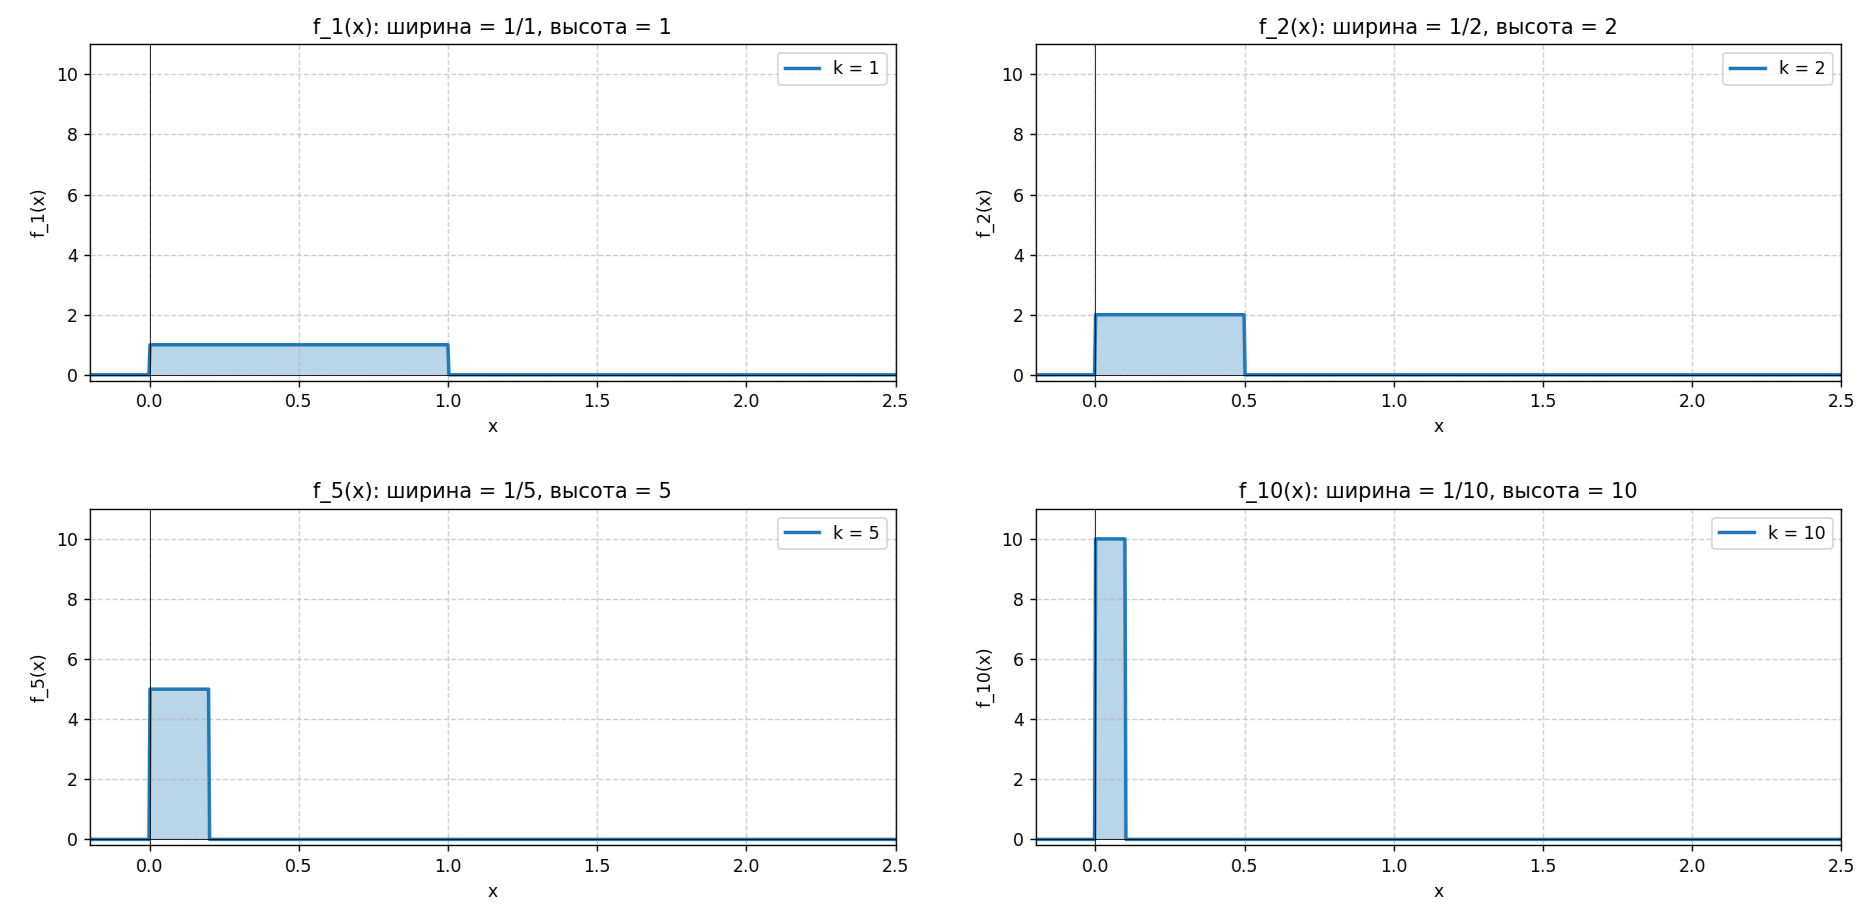
\includegraphics[width=0.6\linewidth]{pics/1.png}
        \caption{}
        \label{fig:enter-label}
    \end{figure}
2)$f_\varepsilon=\dfrac{\varepsilon}{\pi(x^2+\varepsilon^2)}, \quad \varepsilon\to+0$
$$\int\limits_{-a}^{a}\frac{\varepsilon}{\pi(x^2+\varepsilon^2)}\dd x=\frac{1}{\pi}\arctan\frac{x}{\varepsilon}\bigg|_{-a}^{a}=\frac{2}{\pi}\arctan\frac{a}{\varepsilon}\xrightarrow[\varepsilon\to+0]{}1$$
$$\frac{2}{\pi}\arctan\frac{a}{\varepsilon}\xrightarrow{a\to+\infty}1$$
\lbpn{fact}{$$\frac{\varepsilon}{\pi(x^2+\varepsilon^2)}\xrightarrow[\varepsilon\to+0]{}\delta(x)$$}
3)$f_t(x)=\frac{1}{\sqrt{\pi t}}e^{-\frac{x^2}{t}}, \quad t>0, t\to+0$
$$\frac{1}{\sqrt{\pi t}}\int\limits_{-a}^{a}e^{-\frac{x^2}{t}}\dd x=\frac{1}{\sqrt{\pi}}\int\limits_{-a/\sqrt{t}}^{a/\sqrt{t}}e^{-y^2}\dd y\xrightarrow{t\to+0}1$$
\end{myexample}
\begin{myexe}
    $$\frac{\sin(Nx)}{\pi x}\xrightarrow{N\to+\infty}\delta(x)$$
Пусть $\varphi\in D(\mathbb{R})$. Тогда
\[
\left\langle \frac{\sin(Nx)}{\pi x},\varphi\right\rangle
= \int_{\R} \frac{\sin(Nx)}{\pi x}\,\varphi(x)\,dx.
\]
Делаем замену переменной $t = Nx$:
\[
\int_{\R} \frac{\sin(Nx)}{\pi x}\,\varphi(x)\,dx
= \int_{\R} \frac{\sin t}{\pi t}\,\varphi\!\left(\frac{t}{N}\right)dt.
\]
Так как $\varphi$ непрерывна и компактно поддержана, то
$\varphi(t/N)\to\varphi(0)$ равномерно по $t$ на носителе интеграла при $N\to\infty$.
Используя доминированную сходимость и известный интеграл Дирихле
\[
\int_{\R} \frac{\sin t}{\pi t}\,dt = 1,
\]
получаем
\[
\int_{\R} \frac{\sin(Nx)}{\pi x}\,\varphi(x)\,dx
\xrightarrow[N\to\infty]{}
\varphi(0)\int_{\R} \frac{\sin t}{\pi t}\,dt
= \varphi(0).
\]
Следовательно,
\[
\frac{\sin(Nx)}{\pi x} \xrightarrow[N\to\infty]{\DDR} \delta(x) \]


\end{myexe}
\subsection{Носитель обобщенной функции}
\begin{mydef}
    Пусть $f\in\DDR$, сужение $f$ на интервал $(a,b)$:
    $$f|_{(a,b)}=0\Leftrightarrow(f,\phi)=0 \quad \forall \phi\in\DR: \, \supp\phi\subset(a,b)$$
\end{mydef}
\begin{mydef}
    Пусть $f\in\DDR$
    $$\supp f := \R \backslash \{x\in\R: \exists \text{ окрестность }O(x): f|_{O(x)}=0\}$$
    $\supp f$ - замкнутый.
\end{mydef}
\begin{mylemma}
    Пусть $f\in\DDR, \supp f\subset[A, B]$, пусть $\psi\in\DR, \supp \psi\subset[C, D]$
    $$[A,B]\cap[C, D]=\emptyset \Rightarrow (f, \psi)=0$$
\end{mylemma}
\begin{myproof}
    Если $x\in[C, D]$, т.е. $x\not\in[A,B]$ то $\exists O(x):f|_{O(x)}=0 \quad \forall x\in[C, D], \, [C, D]\subset\underset{X}{\cup}O(x)$-покрытие $[C,D]$ этими окрестностями. $[C, D]$-компакт $\Rightarrow [C, D]\subset\cup_{j=1}^{N}\theta(x_j)$ - конечное подпокрытие.
    Разбиение единицы, подчинённое этому покрытию: 
    $$\{\xi_j\}_{j=1}^{N}, \, \xi_j\in\Cinf_0(\R), \sum_{j=1}^{N}\xi_j(x)=1 \quad \forall x\in[C, D], \, \supp \xi_j\subset O(x_j)$$
    $$(f, \psi)=(f, \sum_{j=1}^{N}\xi_j\psi)=\sum_{j=1}^{N}(f, \xi_j\psi)=0, \, \text{т.к. } \supp(\xi_j\psi)\subset O(x_j)(\text{т.к. }\xi_j\psi\in\DR)$$
\end{myproof}
\begin{mytheorem}
    Пусть $f\in\DDR, \supp f$ - компактный, пусть $m\in\N_0, \exists g\in\C(\R): \, f=g^{(m)}$(производная в смысле обобщенной функции)
\end{mytheorem}
\begin{myproof}
    без доказательства
\end{myproof}
\begin{myexe}
    $\exists f\in\DDR, \, f\neq g^{(m)} \, \forall m\in \N_0, \forall g\in\C(\R)$(если не накладывать условие ограниченности носителя)
Рассмотрим распределение $F$, являющееся «первой интегральной
первой производной» от дельта–функции:
\[
F' = \delta, \quad\text{то есть}\quad
\langle F,\varphi'\rangle = -\langle\delta,\varphi\rangle = -\varphi(0)
\quad \forall\,\varphi\in \DR.
\]
По определению производной в $\DDR$ это корректно задаёт
некоторое распределение $F\in \DDR$.

Предположим, что существует непрерывная функция $g\in \C(\R)$
и $m\in\N_0$ такие, что
\[
F = g^{(m)} \quad\text{в } \DDR.
\]
Тогда
\[
\delta = F' = g^{(m+1)}.
\]
Но $g^{(m+1)}$ как производная непрерывной функции есть регулярное
распределение:
\[
\langle g^{(m+1)},\varphi\rangle
= (-1)^{m+1}\int_{\R} g(x)\,\varphi^{(m+1)}(x)\,dx,
\]
а дельта–функция $\delta$ — сингулярное распределение, не задаваемое
никакой локально интегрируемой функцией.
Поэтому равенство $g^{(m+1)}=\delta$ невозможно, и
наше предположение неверно.

Следовательно, $F$ не может быть производной любого порядка
от непрерывной функции $g$:
\[
F \neq g^{(m)} \quad \forall\,m\in\N_0,\ \forall\,g\in C(\R).
\]
Таким образом, требуемое распределение существует, например $f=F$.
\end{myexe}
\begin{mytheorem}
    $$f\in\DDR, \supp f = \{0\} \Rightarrow\exists k\in \N_0, c_0, c_1, \dots c_k \in C \quad f=\sum_{j=0}^{k}c_j\delta^{(j)}$$
\end{mytheorem}
\begin{myexe}
    Доказать эту теорему используя предыдущую и упраженение из 1.3.4
1) Так как $\supp f$ компактен, по теореме 1.2 существует
$m\in\mathbb N_0$ и $g\in C(\mathbb R)$ такие, что
\[
f = g^{(m)} \quad\text{в смысле распределений.}
\tag{1}
\]

2) Из $\supp f=\{0\}$ следует, что $f(\varphi)=0$ для всякой
$\varphi\in D(\mathbb R)$ с $\supp\varphi\subset(-\infty,0)$ или
$\supp\varphi\subset(0,\infty)$. По (1)
\[
0 = \langle f,\varphi\rangle = \langle g^{(m)},\varphi\rangle
= (-1)^m\int_{\mathbb R} g(x)\varphi^{(m)}(x)\,dx.
\]
Так как $\varphi$ на этих интервалах произвольна, получаем
\[
g^{(m)}(x)=0 \quad \text{на }(-\infty,0)\ \text{и на }(0,\infty)
\]
в обычном (классическом) смысле.

По упражнению 1.3.4, из $g^{(m)}=0$ на интервале следует, что $g$
на этом интервале — многочлен степени $<m$. Следовательно,
существуют многочлены $P_-,P_+$ степени $<m$ такие, что
\[
g(x)=
\begin{cases}
P_-(x), & x<0,\\[1mm]
P_+(x), & x>0.
\end{cases}
\tag{2}
\]
Так как $g$ непрерывна на всей $\mathbb R$, получаем ещё, что
$P_-(0)=P_+(0)$.

3) Разложим $P_-,P_+$ в окрестности нуля:
\[
P_-(x)=\sum_{j=0}^{m-1} a_j^- x^j,\qquad
P_+(x)=\sum_{j=0}^{m-1} a_j^+ x^j.
\]

Рассмотрим действие $f$ на произвольной $\varphi\in D(\mathbb R)$.
По (1) и (2):
\[
\langle f,\varphi\rangle
= (-1)^m\int_{-\infty}^{0} P_-(x)\varphi^{(m)}(x)\,dx
 +(-1)^m\int_{0}^{\infty} P_+(x)\varphi^{(m)}(x)\,dx.
\tag{3}
\]

Интегрируем по частям в каждом интеграле $m$ раз.
Так как $P_\pm$ многочлены степени $<m$, после $m$‑кратной
интеграции по частям подынтегральные выражения исчезают, и остаются
только граничные члены при $x=0$ (на $\pm\infty$ всё обнуляется из-за
компактного носителя $\varphi$). В итоге получаем
\[
\langle f,\varphi\rangle
= \sum_{j=0}^{m-1} c_j\,\varphi^{(j)}(0),
\tag{4}
\]
где коэффициенты $c_j$ выражаются через $a_j^\pm$ (их точный вид нам не
нужен).

4) Но по определению производной дельта-функции
\[
\langle \delta^{(j)},\varphi\rangle = (-1)^j \varphi^{(j)}(0),
\]
поэтому из (4)
\[
\langle f,\varphi\rangle
= \sum_{j=0}^{m-1} c_j\,\varphi^{(j)}(0)
= \sum_{j=0}^{m-1} c_j' \,\langle \delta^{(j)},\varphi\rangle
= \left\langle \sum_{j=0}^{m-1} c_j'\,\delta^{(j)},\varphi\right\rangle
\]
для всех $\varphi\in D(\mathbb R)$.

Следовательно, в $D'(\mathbb R)$
\[
f = \sum_{j=0}^{m-1} c_j'\,\delta^{(j)}.
\]
Обозначив $k=m-1$ и переименовав коэффициенты, получаем искомое
представление
\[
f = \sum_{j=0}^{k} c_j\,\delta^{(j)}.\]
\end{myexe}
\section{Прямое произведение обобщенных функций}
\subsection{Пространство \texorpdfstring{$\ddR$}{ } }
\begin{mydef}
    $$\phi\in\dR \Leftrightarrow \supp \phi - \text{ компакт}, \, \phi\in\Cinf(\R^n)$$
    $\phi: \R^n\longrightarrow\C$
\end{mydef}
Шар: $B_R=B_R(0)=\{x\in\R^n: |x|<R\}$.
\begin{mydef}
    $$\phi_k\xrightarrow{\dR}\phi\quad\Leftrightarrow\begin{cases} 1)\exists R: \supp \phi_k\subset B_R, \supp \phi \subset B_R \\ 2)\D^\alpha\phi_k \xrightarrow[k\to+\infty]{}\D^\alpha\phi -\text{ равномерно, }\forall \text{ мультииндексов }\alpha \end{cases}$$
\end{mydef}
$\alpha=(\alpha_1, \alpha_2, \dots), \D^\alpha=\dfrac{\partial^{\alpha_1}\partial^{\alpha_2}\dots\partial^{\alpha_n}}{\partial x_1^{\alpha_1}\partial x_2^{\alpha_2}\dots\partial x_n^{\alpha_n}}$
\begin{mydef}
    $$f\in\ddR \Leftrightarrow f - \text{ линейный непрерывный функционал на } \dR$$
\begin{itemize}
    \item $(\beta f, \phi)=(f, \beta\phi) \quad \beta\in\Cinf(\R^n) $
    \item $(\D^\alpha f, \phi)=(-1)^{|\alpha|}(f, \D^\alpha\phi) \quad |\alpha|=\alpha_1+\alpha_2+\dots+\alpha_n$
    \item $f_k\xrightarrow{\ddR}f\Leftrightarrow(f_k, \phi)\longrightarrow(f,\phi) \quad \forall\phi\in\dR$
\end{itemize}
\end{mydef}
\begin{myexample}
    $S$ - гладкая поверхность
    $$(\delta_S, \phi)=\int\limits_S\phi(x)\dd S(x)$$
$\delta_S\in\ddR$
\end{myexample}

\subsection{Прямое произведение}
$f, g\in\DDR \quad \int\limits_{\R^2}f(x)g(y)\phi(x, y)\dd x\dd y$ - это то, чего мы пытаемся добится прямым произведением.
\begin{mylemma}
    \lbpn{second}{Пусть $\phi\in\D(\R^2)$, пусть $x\in\R$ - фиксированный.
    $$\frac{\phi(x+h, y) - \phi(x, y)}{h}\xrightarrow[h\to0]{\D(\R_y)}\frac{\partial \phi}{\partial x}(x,y)$$}
\end{mylemma}
\begin{myproof}
    

\begin{tikzpicture}[scale=1.2, thick, >=Stealth]

\draw[->] (0,0) -- (6,0) node[below right] {$x$};
\draw[->] (0,0) -- (0,5) node[above left] {$y$};


\node[below left] at (0,0) {$0$};


\def\A{1}
\def\B{5}
\def\C{0.5}
\def\D{4}

\draw[blue, thick] (\A,\C) rectangle (\B,\D);
\node[blue, above] at ({\A+(\B-\A)/2}, \D) {прямоугольник};


\node[below] at (\A, \C) {$A$};
\node[below] at (\B, \C) {$B$};
\node[left] at (\A, \C) {$C$};
\node[left] at (\A, \D) {$D$};

\draw[red, thick, pattern=north east lines, pattern color=red] 
  (1.5,1.2) -- (2.5,2.0) -- (3.2,1.8) -- (4.2,3.0) -- (4.0,3.5) -- (2.0,2.5) -- cycle;


\node[purple, left] at (4.5, 2.5) {$\supp \phi$};
\draw[->, thick, purple] (4.5, 2.5) -- (2.8, 2.0);


\def\x{1.8}
\def\h{1.8}
\def\xph{3.6}

\draw[dashed, thick, green!50!black] (\x, \C) -- (\x, \D);
\draw[dashed, thick, green!50!black] (\xph, \C) -- (\xph, \D);


\node[below, green!50!black] at (\x, \C) {$x$};
\node[below, green!50!black] at (\xph, \C) {$x+h$};

\end{tikzpicture} \\
$\supp\phi\subset[A, B]\times[C, D], \,$ делаем сужение на вертикальные прямые: 
$$\supp\frac{\phi(x+h, \cdot) - \phi(x, \cdot)}{h}\subset [C, D] , \quad \supp\frac{\partial\phi(x, \cdot)}{\partial x}\subset[C, D]$$
$$\bigg|\phi(x+h, y) - \phi(x, y) - h\dfrac{\partial\phi(x, y)}{\partial x}\bigg|\leq(\text{ряд тейлора}) h^2\underset{y\in[C,D]}{\max}\bigg|\dfrac{\partial^2\phi(x,y)}{\partial x^2}\bigg|\leq h^2\underset{\R^2}{\max}\bigg|\dfrac{\partial^2\phi}{\partial x^2}\bigg|$$
Деля на $h$ обе части равенства: 
$$\bigg|\dfrac{\phi(x+h, y) - \phi(x, y)}{h}-\dfrac{\partial \phi(x,y)}{\partial x}\bigg|\leq h\underset{\R^2}{\max}\bigg| \dfrac{\partial^2\phi(x,y)}{\partial x^2}\ \bigg|\Rightarrow$$
$$\Rightarrow \dfrac{\phi(x+h, \cdot)-\phi(x,\cdot)}{h}\rightarrow\frac{\partial\phi(x,\cdot)}{\partial x} \text{ равномерно на всей оси}$$
Для производных аналогично:
$$\dfrac{\dfrac{\partial^k\phi}{\partial y^k}(x+h, y)-\dfrac{\partial^k\phi}{\partial y^k}(x, y)}{h}\xrightarrow[h\to0]{}\dfrac{\partial^{k+1}\phi(x,y)}{\partial x\partial^ky} \text{ равномерно}$$
\end{myproof}
\begin{mylemma}
    Пусть $g\in\DDR, \, f\in\D(\R^2)$. 
    $$\psi(x):=(g,\phi(x,\cdot))\Rightarrow\psi\in\DR \quad \psi^{(l)}(x)=\bigg(g, \frac{\partial^l\phi}{\partial x^l}(x, \cdot)\bigg)$$
Примечание: $g$ действует на $\cdot$.
\end{mylemma}
\begin{myproof}
    $\supp\phi\subset[A, B]\times[C, D] \Rightarrow \supp\psi\subset[A, B]$
    $$\dfrac{\psi(x+h)-\psi(x)}{h}=\bigg(g, \dfrac{\phi(x+h, \cdot)-\phi(x,\cdot)}{h}\bigg)\xrightarrow[h\to0]{\text{лемма 1.1}}\bigg(g, \dfrac{\partial \phi(x,\cdot)}{\partial x}\bigg) \Rightarrow$$
    $$\Rightarrow\exists\psi'(x)=\bigg(g, \dfrac{\partial\phi(x,\cdot)}{\partial x}\bigg)$$
    Далее по индукции получаем, что $\exists \psi^{(l)}(x)=\bigg(g,\dfrac{\partial^l \phi(x, \cdot)}{\partial x^l}\bigg)$
\end{myproof}
\begin{mylemma}
    Пусть $g\in\DDR, \, \phi_k\in\D(\R^2)$, пусть $\phi_k\xrightarrow{\D(\R^2)}0$
    $$\psi_k=(g, \phi_k(x, \cdot))\Rightarrow\psi_k\xrightarrow{\DDR}0$$
\end{mylemma}
\begin{myproof}
    $\supp\phi_k\subset[A, B]\times[C, D] \Rightarrow \supp\psi_k\subset[A, B]$
    Достаточно доказать, что $\psi_k\xrightarrow[k\to+\infty]{}0$ равномерно(в силу леммы 1.2(потому что производные строятся точно так же)). Пойдём от противного(сходится неравномерно): $\exists\varepsilon>0, \exists k_j(\to+\infty),x_j:|\psi_{k_j}(x_j)|\geq\varepsilon \Leftrightarrow |(g,\phi_{k_j}(x_j, \cdot))|\geq\varepsilon$
    Пусть $w_j(y)=\phi_{k_j}(x_j, y), \quad w_j\xrightarrow{\DR}0, \supp w_j\subset[C,D]$ \\
    $$w_j^{(m)}=\dfrac{\partial^m\phi_{k_j}}{\partial y^m}(x_j, y)\xrightarrow[\text{равномерно}]{}0 \Rightarrow (g, w_j)\longrightarrow 0(\text{ потому что g-непрерывный функционал})$$
    Но, по предположению $|(g, w_j)|\geq\varepsilon$ значит противоречие.
\end{myproof}
\begin{myproof}
    Пусть $f, g \in \DDR$. Прямое произведение:
    $$(f(x)g(y), \phi)=(f(x),(g, \phi(x,\cdot)))$$
\end{myproof}
Корректность следует из леммы 1.2, линейность очевидна, а непрерывность следует из леммы 3, $f(x)g(y)\in\D(\R^2)$
\begin{mytheorem}
    Прямое произведение - коммутативно: $f(x)g(y)=g(y)f(x)$
    $$(f(x),(g,\phi(x,\cdot)))=(g(y),(f,\phi(\cdot,y)))$$
\end{mytheorem}
\begin{myproof}
    без доказательства
\end{myproof}
\begin{myremark}
    1) $\delta(x)\delta(y)=\delta(x,y)$\\
    2)$\dfrac{\partial}{\partial x}\bigg(f(x)g(y)\bigg)=f'(x)g(y)$ \\
    $\dfrac{\partial}{\partial y}\bigg(f(x)g(y)\bigg)=f(x)g'(y)$ \\
    $\bigg(\dfrac{\partial}{\partial y}\bigg(f(x)g(y)\bigg), \phi\bigg)=-\bigg(f(x)g(y), \dfrac{\partial \phi}{\partial y}\bigg)=-\bigg(f(x), \bigg(g,\dfrac{\partial\phi(x,\cdot)}{\partial y}\bigg)\bigg)=\bigg(f(x),(g',\phi(x,\cdot))\bigg)=\bigg(f(x)g'(y),\phi\bigg)$ \\
    3) $f\in\ddR, g\in\D'(\R^m)$ \\
    $f(x)g(y)\in\D'(\R^{n+m})$
\end{myremark}
\section{Свёртка}
\subsection{Определение}
Пусть $\phi, \psi \in \DR$, мы хотим под сверткой понимать что то подобное: 
$$(\phi\ast\psi)(x)=\int\limits_\R\phi(x-y)\psi(y)\dd y=\begin{vmatrix}
    x-y=z \\
    y=x-z
\end{vmatrix}=\int\limits_\R\phi\psi(x-z)\dd z=(\psi\ast\phi)(x)$$
Ещё мы хотим: $\phi\ast\psi\in\DR$, $(\phi\ast\psi)'=\phi'\ast\psi=\phi\ast\psi'$
\begin{mydef}
    Пусть $f\in\DDR, \,\, \phi\in\DR$. Тогда свёртка:
    $$(f\ast\phi)(x)=(f,\phi(x-\cdot))$$
\end{mydef}
\begin{myexample}
    $$\delta\ast\phi=\phi$$
\end{myexample}
\begin{mytheorem}
    Пусть $f\in\DDR, \,\, \phi\in\DR \Rightarrow$
    $$\Rightarrow f\ast\phi\in\Cinf(\R), \quad (f\ast\phi)'=f'\ast\phi=f\ast\phi'$$ 
\end{mytheorem}
\begin{myproof}
    Пусть $x\in\R$, 
    $$\dfrac{\phi(x+h-\cdot)-\phi(x-\cdot)}{h}\xrightarrow[h\to0]{\DR}\phi'(x-\cdot) \quad \text{доказательство аналогично \ref{second}}$$
    $$\dfrac{(f\ast\phi)(x+h)-(f\ast\phi)(x)}{h}=\dfrac{1}{h}\bigg((f,\phi(x+h-\cdot))-(f,\phi(x-\cdot))\bigg)$$
    $$=\bigg(f, \dfrac{\phi(x+h-\cdot)-\phi(x-\cdot)}{h}\bigg)\xrightarrow[h\to0]{}(f,\phi'(x-\cdot))=(f\ast\phi')(x) \Rightarrow$$
    $$\Rightarrow \exists (f\ast\phi)'(x)=(f\ast\phi')(x) \xRightarrow{\text{по индукции}}(f\ast\phi)^{(m)}(x)=(f\ast\phi^{(m)})(x) \Rightarrow$$
    $$\Rightarrow \quad f\ast\phi\in\Cinf(\R)$$
Очевидно, что $\phi'(x-y)=-\phi'_y(x-y)$. Тогда 
$$(f\ast\phi')(x)=(f,\phi'(x-\cdot))=-(f,\phi'_y(x-\cdot))=(f',\phi(x-\cdot))$$
Последнее равенство обусловлено тем, что обобщенная функция $f$ действует по переменной $\cdot$.
\end{myproof}
\subsection{Замечания}
\begin{myremark}
    1) $f\in\ddR, \,\, \phi\in\dR$, $(f\ast\phi)(x)=(f,\phi(x-\cdot))$
    $$f\ast\phi\in\Cinf(\R), \quad \D^\alpha(f\ast\phi)=(\D^\alpha f\ast\phi)=(f\ast\D^\alpha\phi)$$
    2) Можно ли определить свёртку от двух обобщённых функций, вообще говоря нет, потому что как минимум оно может быть не компактно: $\phi=\psi=1$. Тогда 
    $$1\ast 1=\int\limits_R 1\dd y=+\infty$$
    Пусть $f, g\in\DDR$. Что бы мы ожидали получить зная понятие регулярных функций: 
    $$(f\ast g, \phi)=\int\limits_\R\int\limits_\R f(x-y)g(y)\phi(x)\dd x\dd y=|x=y+z|=\int\limits_\R\int\limits_\R f(z)g(y)\phi(y+z)\dd y \dd z$$
    $$(f\ast g,\phi)=(f(x)g(y),\phi(x+y))$$
    Но тут есть проблема: $\phi(x,y):=\phi(x+y)$, здесь носитель не компактный, это можно увидеть на графике:
 \begin{figure}[H]
        \centering
        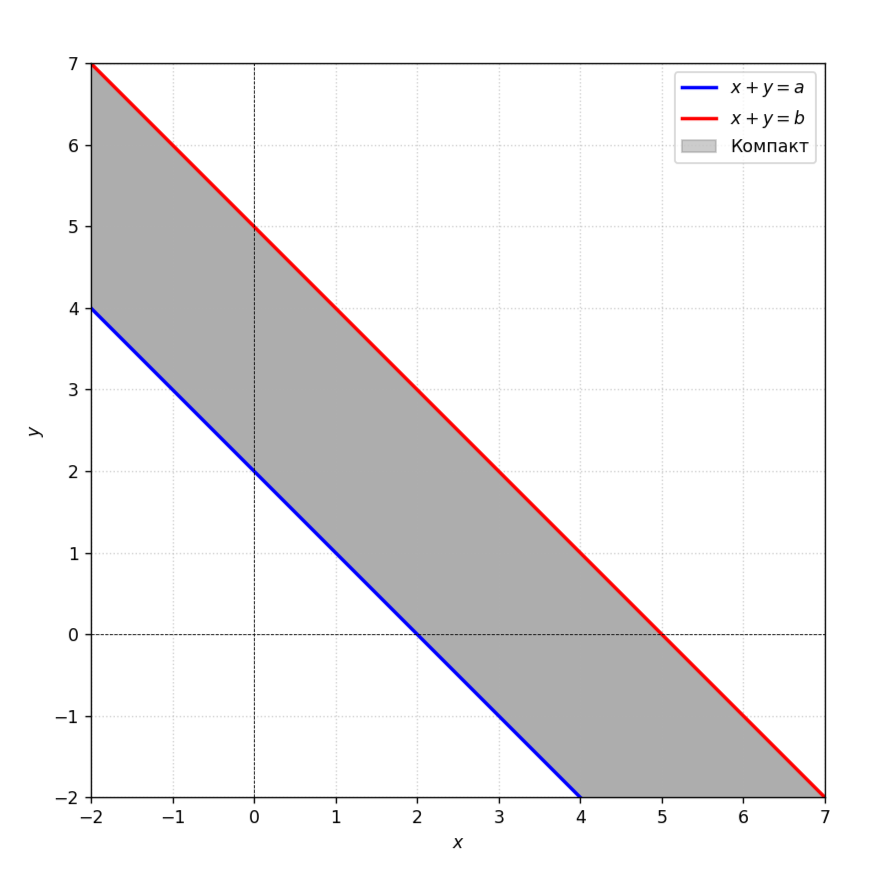
\includegraphics[width=0.6\linewidth]{pics/2.png}
        \caption{}
        \label{fig:enter-label}
    \end{figure}
Поэтому такое определение нам не подойдёт.
\end{myremark}
\begin{myexe}
    1) $\exists \eta\in\DR: \quad \eta|_{[a,b]}=1$. Выглядит она вот так:
    \begin{figure}[H]
        \centering
        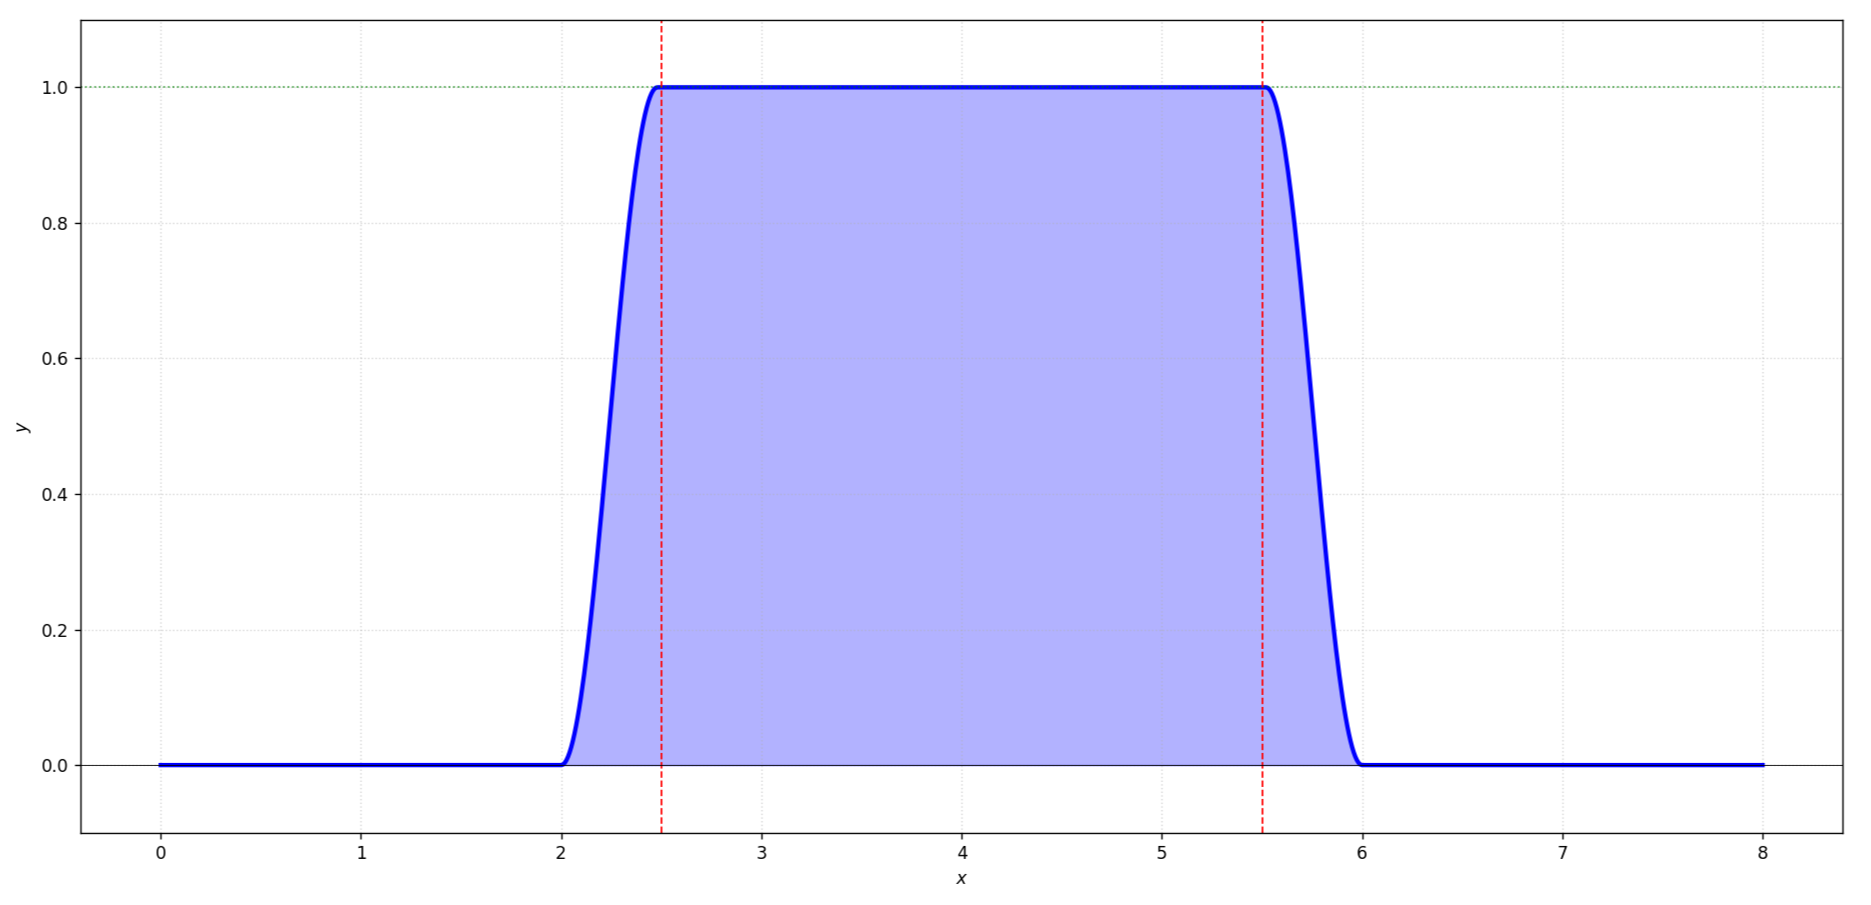
\includegraphics[width=0.6\linewidth]{pics/3.png}
        \caption{}
        \label{fig:enter-label}
    \end{figure}
    2) Пусть $f\in\DDR, \quad \supp f \subset (a, b)$ \\
    Пусть $\eta\in\DR: \quad \eta|_[a,b]=1 \Rightarrow \eta f=f$\\
1)
Рассмотрим вспомогательную функцию
\[
\psi(t) =
\begin{cases}
e^{-1/t^{2}}, & t>0,\\
0,            & t \le 0.
\end{cases}
\]
Нетрудно проверить, что $\psi \in \C^{\infty}(\R)$ и
$\psi^{(k)}(0)=0$ для всех $k \in \N\cup\{0\}$, то есть
$\psi$ ``плоская'' в нуле.

Определим сглаженную ступенчатую функцию
\[
\theta(t) = \frac{\psi(t)}{\psi(t)+\psi(-t)}.
\]
Тогда $\theta \in C^{\infty}(\R)$,
\[
\theta(t)=
\begin{cases}
0, & t \ll 0,\\
1, & t \gg 0,
\end{cases}
\]
и все переходы происходят бесконечно гладко.

Зафиксируем $\varepsilon>0$ так, чтобы $a-\varepsilon < a < b < b+\varepsilon$,
и положим
\[
\eta(x) = \theta\bigl(x-(a-\varepsilon)\bigr)\,
          \theta\bigl((b+\varepsilon)-x\bigr).
\]
Тогда $\eta \in \C^{\infty}(\R)$ как произведение гладких функций.
Из определения $\theta$ видно, что
\[
\eta(x) =
\begin{cases}
0, & x \le a-\varepsilon \ \text{или} \ x \ge b+\varepsilon,\\
1, & x \in [a,b],
\end{cases}
\]
то есть $\eta$ имеет компактный носитель, лежащий в
$(a-\varepsilon,\, b+\varepsilon)$, и удовлетворяет $\eta|_{[a,b]} \equiv 1$.
Следовательно, $\eta \in \DR$ и обладает требуемыми
свойствами.

\bigskip


2) По определению произведения распределения на гладкую функцию
\[
\langle \eta f,\varphi\rangle = \langle f,\eta\varphi\rangle
\quad \forall\,\varphi\in \DR.
\]
Так как $\supp f\subset(a,b)$, то для любой $\varphi$ имеем
\[
\langle f,\varphi\rangle = \langle f,\varphi\cdot 1_{(a,b)}\rangle,
\]
и на $(a,b)$ выполняется $\eta(x)\equiv 1$, значит
\[
\eta(x)\varphi(x) = \varphi(x)\quad \text{при } x\in\supp f.
\]
Следовательно,
\[
\langle \eta f,\varphi\rangle
= \langle f,\eta\varphi\rangle
= \langle f,\varphi\rangle
\quad \forall\,\varphi\in D(\R),
\]
то есть $\eta f$ и $f$ действуют одинаково на всех тестовых функциях,
а значит, $\eta f = f$ как элементы $\DDR$.

\end{myexe}
Определим свёртку обобщенных функций правильно.
\begin{mydef}
    Пусть $f, g\in\DDR \quad \supp \subset(a, b)$. 
    $$(f\ast g, \phi)=(f(x)g(y),\underbrace{\phi(x+y)\eta(x)}_{\in\D(\R^2)})$$
\end{mydef}
На рисунке с носителем, мы таким образом вырезаем параллелограмм.
\begin{myexe}
    $\phi_k\xrightarrow{\DR}0 \quad \Rightarrow \quad \phi_k(x+y)\eta(x)\xrightarrow{\D(\R^2)}0$ \\
    \begin{enumerate}
\item[(i)] существует компакт $K_\varphi\subset\mathbb R$, такой что 
$\operatorname{supp}\varphi_k\subset K_\varphi$ для всех $k$;
\item[(ii)] для любого целого $m\ge0$ выполнено
\[
\sup_{x\in\R}\bigl|\varphi_k^{(m)}(x)\bigr|\xrightarrow[k\to\infty]{}0.
\]
\end{enumerate}

Пусть $\operatorname{supp}\eta\subset K_\eta$, где $K_\eta\subset\R$ — компакт.
Рассмотрим $\psi_k(x,y)=\varphi_k(x+y)\eta(x)$.

\smallskip

\noindent\textit{1) Общий компакт для носителей.}
Если $\psi_k(x,y)\neq0$, то одновременно $\eta(x)\neq0$ и $\varphi_k(x+y)\neq0$,
следовательно
\[
x\in K_\eta,\qquad x+y\in K_\varphi.
\]
Отсюда $y\in K_\varphi - x\subset K_\varphi-K_\eta$, где
\[
K_\varphi-K_\eta := \{t-s:\ t\in K_\varphi,\ s\in K_\eta\}.
\]
Таким образом,
\[
\operatorname{supp}\psi_k
\subset K_\eta\times (K_\varphi-K_\eta) =: K,
\]
и $K\subset\R^2$ — компакт, не зависящий от $k$.

\smallskip

\noindent\textit{2) Равномерное стремление производных к нулю.}
Возьмём произвольный многоиндекс $\alpha=(\alpha_1,\alpha_2)$
и вычислим $\D^\alpha_{x,y}\psi_k(x,y)$.
Поскольку $\psi_k(x,y)=\varphi_k(x+y)\eta(x)$, по формуле Лейбница и цепному правилу имеем
\[
\D^\alpha_{x,y}\psi_k(x,y)
=
\sum_{\beta\le\alpha} C_{\alpha,\beta}\,
\frac{d^{\beta_1+\beta_2}\varphi_k}{dt^{\beta_1+\beta_2}}(x+y)\,
\frac{d^{\alpha_1-\beta_1}\eta}{dx^{\alpha_1-\beta_1}}(x),
\]
где сумма берётся по всем $\beta=(\beta_1,\beta_2)$ с $\beta\le\alpha$,
а $C_{\alpha,\beta}$ — некоторые константы.

Так как $\eta\in\mathcal \DR$, её производные
$\eta^{(j)}$ ограничены на $\R$.
Из (ii) вытекает, что для любого $m\ge0$
\[
\sup_{t\in\R}\bigl|\varphi_k^{(m)}(t)\bigr|\xrightarrow[k\to\infty]{}0.
\]
Следовательно для каждого $\alpha$
\[
\sup_{(x,y)\in\R^2}\bigl|D^\alpha\psi_k(x,y)\bigr|
\le
\sum_{\beta\le\alpha}|C_{\alpha,\beta}|\,
\Bigl(\sup_t|\varphi_k^{(\beta_1+\beta_2)}(t)|\Bigr)\,
\Bigl(\sup_s|\eta^{(\alpha_1-\beta_1)}(s)|\Bigr)
\xrightarrow[k\to\infty]{}0.
\]

Итак, для любого многоиндекса $\alpha$ производные $\D^\alpha\psi_k$ равномерно
стремятся к нулю, а носители $\psi_k$ лежат в одном компакте $K$.
По определению топологии в $\D(\R^2)$ это означает
$\psi_k\to0$ в $\D(\R^2)$.

\end{myexe}
\begin{myexe}
    Определение не зависит от выбора $\eta$. \\
    Пусть $f,g \in \mathcal \DDR$ имеют компактные носители
\[
\supp f \subset K_f,\qquad \supp g \subset K_g,
\]
где $K_f,K_g \subset \R$ --- компакты. Тогда
\[
\supp(f\otimes g) \subset K_f \times K_g.
\]

Пусть $\eta_1,\eta_2 \in \DR$ такие, что
\[
\eta_1(x) = \eta_2(x) = 1 \quad \text{для всех } x \in K_f.
\]
Определим свёртку с помощью $\eta_i$ по формуле
\[
(f*g,\varphi)_{\eta_i} := (f\otimes g,\ \varphi(x+y)\eta_i(x)),
\qquad \varphi \in \DR,\ i=1,2.
\]

Рассмотрим разность:
\[
R(\varphi)
:= (f*g,\varphi)_{\eta_1} - (f*g,\varphi)_{\eta_2}
= (f\otimes g,\ \Phi(x,y)),
\]
где
\[
\Phi(x,y) := \varphi(x+y)\bigl(\eta_1(x)-\eta_2(x)\bigr).
\]

Заметим, что при $x\in K_f$ выполнено $\eta_1(x)=\eta_2(x)$, поэтому
\[
\eta_1(x)-\eta_2(x)=0 \quad \text{для всех } x\in K_f.
\]
Отсюда
\[
\Phi(x,y)=0 \quad \text{для всех } (x,y)\in K_f\times K_g.
\]
Так как
\(
\supp(f\otimes g)\subset K_f\times K_g,
\)
получаем, что $\Phi$ тождественно равна нулю в некоторой окрестности
$\supp(f\otimes g)$.

По определению распределения, если $\Psi\in\D(\R^2)$ и
$\Psi \equiv 0$ в окрестности $\supp T$, то $(T,\Psi)=0$.
Применяя это к $T=f\otimes g$ и $\Psi=\Phi$, имеем
\[
R(\varphi) = (f\otimes g,\Phi)=0.
\]

Следовательно, для любой $\varphi\in\DR$
\[
(f*g,\varphi)_{\eta_1} = (f*g,\varphi)_{\eta_2},
\]
то есть определение свёртки $f*g$ не зависит от выбора функции $\eta$.
\end{myexe}
\begin{myremark}
    1) Пусть $f,g\in\DDR, \quad \supp g\subset(c, d)$, то 
    $$(f\ast g, \phi)=(f(x)g(y), \phi(x+y)\eta(y))$$
    Здесь уже $\eta|_{[c, d]}=1$ \\
    2) $\supp f, \, \supp g$ - компактные, то можно определить и так и так: $f\ast g=g\ast f$ \\
    3) $\delta\ast f=f$ \\
    4) Можно так же дифференцировать: $(f\ast g)'=f'\ast g=f\ast g'$. \\
    $$(\{\text{обобщённые функции с компактным }\supp\}, \ast) - \text{ коммутативная алгебра с единицей}$$
    Анти-пример - $\theta, \delta', 1$ и это не будет алгеброй: \\
    $(\theta\ast \delta')\ast 1=(\theta\ast\delta)'\ast1=\theta'\ast1=\delta\ast1=1$ \\
    $\theta\ast (\delta'\ast 1)=\theta\ast(\delta\ast1)'=\theta\ast1'=\delta\ast0=0$
\end{myremark}
\section{Пространство Шварца \texorpdfstring{$\SR$}{ }}
\subsection{Пространство быстро убывающих функций \texorpdfstring{$\SR$}{ }}
На $\DDR$ не определить преобразование Фурье, поэтому нужно сузить класс обобщенных функци, но расширить класс основных.
\begin{mydef}
    $$\phi\in\SR \quad \Leftrightarrow \quad \begin{cases}
        1) \phi\in\Cinf(\R) \\
        2)\forall l, m \,\, \exists C_{lm}: \, |x^l\phi^{(m)}|\leq C_{lm} \forall x\in\R
    \end{cases}$$
2 можно записать как $\phi^{(m)}=O(x^{-l}) \quad \forall m, l \,\,\,\, x\to\infty$, т.е. любая производная функции убывает быстрее любой степени.
\end{mydef}
\begin{myremark}
    \lbpn{forth}{$$\phi\in\SR \quad \Rightarrow \quad x\phi\in\SR$$}
    Домножение возможно, т.к. убывает быстрее любой степени и функция так же остаётся гладкой.
\end{myremark}
\begin{myexe}
    1) $\DR\subset\SR$ \\
    2) $e^{-x^2}\in\SR\backslash\DR$ \\
    Зафиксируем любые неотрицательные целые $l,m$.
Рассмотрим функцию
\[
x\longmapsto (|x|)^l\,\varphi^{(m)}(x).
\]
На компакте $K$ производная $\varphi^{(m)}$ непрерывна, следовательно
ограничена, а вне $K$ имеем $\varphi^{(m)}(x)=0$ (так как $\varphi$ тождественно
равна нулю вне $K$). Поэтому
\[
\sup_{x\in\R}(|x|)^l\,|\varphi^{(m)}(x)|<\infty.
\]
Это верно для всех $l,m$, значит $\varphi\in \SR$ по определению
пространства Шварца. Тем самым $\DR\subset \SR$.

\smallskip

\textbf{2)} Рассмотрим функцию $\psi(x)=e^{-x^2}$.

Сначала покажем, что $\psi\in \SR$.
Производные $\psi^{(m)}(x)$ имеют вид
\[
\psi^{(m)}(x)=P_m(x)\,e^{-x^2},
\]
где $P_m$ --- некоторый многочлен степени не выше $2m$.
Это доказывается по индукции по $m$ (правило Лейбница и цепное правило).

Возьмём произвольные $l,m\ge0$.
Имеем
\[
(|x|)^l\,|\psi^{(m)}(x)|
=
(|x|)^l\,|P_m(x)|\,e^{-x^2}.
\]
Произведение многочлена на $e^{-x^2}$ ограничено на $\R$
(экспонента $e^{-x^2}$ убывает быстрее любой степени $|x|$), поэтому
существует константа $C_{l,m}$, такая что
\[
\sup_{x\in\R}(|x|)^l\,|\psi^{(m)}(x)| \le C_{l,m}<\infty.
\]
Следовательно $\psi\in S(\R)$.

Теперь проверим, что $\psi\notin\DR$.
Функция $e^{-x^2}$ нигде не обращается в нуль, то есть
\[
\supp\psi = \overline{\{x:\psi(x)\ne0\}}=\R,
\]
а значит носитель некомпактен. По определению
$\DR$ состоит из гладких функций с \emph{компактным}
носителем, поэтому $\psi\notin\DR$.

Итак, $e^{-x^2}\in S(\R)\setminus\DR$.
\end{myexe}
\begin{mydef}
    $$\phi_k\xrightarrow{\SR}\phi \quad\Leftrightarrow\quad \forall l,m\in \N_0 \,\,\,\, x^l\phi^{(m)}_k(x)\rightarrow x^l\phi^{(m)}(x)\text{ равномерно на } \R$$
\end{mydef}
$\SR$ - метризуемо. Доказательство состоит из двух упражнений: 
\begin{myexe} 
    1)$\rho=\displaystyle\sum\limits_{l,m=0}^{\infty}\dfrac{\underset{\R}{\max}|x^l\phi^{(m)}(x)-x^l\psi^{(m)}(x)|}{2^{l+m}(1+\underset{\R}{\max}|x^l\phi^{(m)}(x)-x^l\psi^{(m)}(x)|)}$. Надо доказать, что это метрика(неотрицательная, невырожденная, неравенство треугольника) \\
    2) $\phi_k\xrightarrow[k\to\infty]{\SR}\phi \quad \Leftrightarrow \quad \rho(\phi_k, \phi) \xrightarrow[k\to\infty]{}0$
\\
Обозначим
\[
a_{l,m}(\varphi,\psi)
:=p_{l,m}(\varphi-\psi)
=\sup_{x\in\mathbb R}|x|^l\,|\varphi^{(m)}(x)-\psi^{(m)}(x)|.
\]
Положим $\theta(t)=\dfrac{t}{1+t}$ при $t\ge0$.
Тогда
\[
\rho(\varphi,\psi)
=
\sum_{l,m}2^{-(l+m)}\,\theta\bigl(a_{l,m}(\varphi,\psi)\bigr).
\]

1)
Очевидно, что $\rho(\varphi,\psi)\ge0$ и
$\rho(\varphi,\psi)=\rho(\psi,\varphi)$.

Если $\rho(\varphi,\psi)=0$, то все слагаемые равны нулю, т.е.
$\theta(a_{l,m}(\varphi,\psi))=0$ для всех $l,m$. Так как $\theta(t)=0$
только при $t=0$, получаем $a_{l,m}(\varphi,\psi)=0$, то есть
\[
\sup_x |x|^l\,|\varphi^{(m)}(x)-\psi^{(m)}(x)|=0
\]
для всех $l,m$. Отсюда $\varphi^{(m)}\equiv\psi^{(m)}$ и, следовательно,
$\varphi=\psi$.

Проверим неравенство треугольника. Для любых
$\varphi,\psi,\chi\in \SR$ и фиксированных $l,m$ имеем
\[
a_{l,m}(\varphi,\chi)
=p_{l,m}(\varphi-\chi)
\le p_{l,m}(\varphi-\psi)+p_{l,m}(\psi-\chi)
=a_{l,m}(\varphi,\psi)+a_{l,m}(\psi,\chi),
\]
так как $p_{l,m}$ --- полунорма.
Функция $\theta(t)=\frac{t}{1+t}$ неотрицательна, возрастает и удовлетворяет
оценке $\theta(u+v)\le\theta(u)+\theta(v)$ при $u,v\ge0$ (легко проверить).
Отсюда
\[
\theta(a_{l,m}(\varphi,\chi))
\le
\theta(a_{l,m}(\varphi,\psi))
+
\theta(a_{l,m}(\psi,\chi)).
\]
Домножая на $2^{-(l+m)}$ и суммируя по $l,m$, получаем
\[
\rho(\varphi,\chi)\le\rho(\varphi,\psi)+\rho(\psi,\chi).
\]
Значит, $\rho$ --- метрика.

\medskip

2) 
\[
\varphi_k\to\varphi \text{ в } \SR
\iff
\forall\,l,m\quad p_{l,m}(\varphi_k-\varphi)\xrightarrow[k\to\infty]{}0.
\tag{*}
\]

\emph{($\Rightarrow$)} Если выполняется (*), то для любых фиксированных $l,m$
\[
p_{l,m}(\varphi_k-\varphi)\to0.
\]
Поскольку функция $\theta(t)=\dfrac{t}{1+t}$ непрерывна и $\theta(0)=0$,
имеем
\[
\theta\bigl(p_{l,m}(\varphi_k-\varphi)\bigr)\to0.
\]
Каждое слагаемое в сумме для $\rho(\varphi_k,\varphi)$ неотрицательно и
ограничено $2^{-(l+m)}$, поэтому при $k\to\infty$ сумма также стремится к
нулю:
\[
\rho(\varphi_k,\varphi)\xrightarrow[k\to\infty]{}0.
\]

\emph{($\Leftarrow$)} Пусть наоборот $\rho(\varphi_k,\varphi)\to0$.
Зафиксируем произвольные $l,m$. Тогда
\[
0\le
2^{-(l+m)}\frac{p_{l,m}(\varphi_k-\varphi)}{1+p_{l,m}(\varphi_k-\varphi)}
\le \rho(\varphi_k,\varphi)\xrightarrow[k\to\infty]{}0,
\]
откуда
\[
\frac{p_{l,m}(\varphi_k-\varphi)}{1+p_{l,m}(\varphi_k-\varphi)}
\xrightarrow[k\to\infty]{}0.
\]
Функция $\theta(t)=\dfrac{t}{1+t}$ строго возрастает на $[0,\infty)$ и
$\theta(t)=0$ только при $t=0$, поэтому из
$\theta\bigl(p_{l,m}(\varphi_k-\varphi)\bigr)\to0$ следует
\[
p_{l,m}(\varphi_k-\varphi)\xrightarrow[k\to\infty]{}0.
\]
Так как $l,m$ были произвольны, выполнено (*), т.е.
$\varphi_k\to\varphi$ в $\SR$.
\end{myexe}
Сущесвтенно, что это пространство - алгебра.
\begin{mylemma}
    Пусть $\phi, \psi\in\SR \quad \Rightarrow \quad \phi\psi\in\SR,\,\, \phi\ast\psi\in\SR$
\end{mylemma}
\begin{myproof}
    С произведением всё очевидно, перемножение так же даёт бесконечно гладкую функицю и так же производные убиывают быстрее любой степени.
    $$(\phi\ast\psi)(x)=\int\limits_\R\phi(x-y)\psi(y)\dd y$$
    Рассмотрим:
    $$x^m(\phi\ast\psi)\underset{((x-y)+y)^m}{=}\int\limits_\R\sum\limits_{k=0}^{m}C^k_m(x-y)^{m-k}\phi(x-y)y^m\psi(y)\dd y$$
Последнее равенство - разложение в бином Ньютона. По определению функции из пространства Шварца: 
    $$|(x-y)^{m-k}\phi(x-y)|\leq C_1 \quad \forall x, y$$
    $$|y^m\psi(y)|\leq\dfrac{C_2}{1+y^2}$$
Тогда получаем: 
$$\bigg|\int\limits_\R(x-y)^{m-k}\phi(x-y)y^m\psi(y)\dd y\bigg|\leq C_1C_2\int\limits_\R\dfrac{\dd y}{1+y^2}<\infty$$
Тогда получаем, что $\phi\ast\psi=O(x^{-m}), \quad x\to\infty$. Для производной все логично:
$$(\phi\ast\psi)^{(j)}=\phi^{(j)}\ast\psi \quad \Rightarrow \quad (\phi\ast\psi)^{(j)}=O(x^{-m}), \quad x\to\infty$$
\end{myproof}
\subsection{Преобразование Фурье}
\begin{mydef}
    Пусть $\phi\in\SR$, преобразование Фурье:
    $$(\F\phi)(\xi)=\widehat{\phi}(\xi)=\frac{1}{\sqrt{2\pi}}\int\limits_\R e^{-i\xi x}\phi(x)\dd x$$
\end{mydef}
Важное свойство заключается в том, что производная тоже гладкая функция и вот как она выглядит(производная по $\xi$):
$$\widehat{\phi}'(\xi)=\frac{1}{\sqrt{2\pi}}\int\limits_\R e^{-i\xi x}(-ix\phi(x))\dd x$$
$$\widehat{\phi}'(\xi)=-i(x\phi)\hat{}\quad (\widehat{\phi})^{(l)}=((-ix)^l\phi)\hat{}$$
$$\widehat{\phi'}=\frac{1}{\sqrt{2\pi}}\int\limits_\R e^{-i\xi x}\phi'\dd x\underset{\text{интегр. по частям}}{=}\frac{i\xi}{\sqrt{2\pi}}\int\limits_\R e^{-i\xi x}\phi(x)\dd x$$
Интегрирование по частям: первый член зануляется из за того, что $\phi$ быстро убывающая.
\lbpn{third}{\[\widehat{\phi'}=i\xi\hat{\phi}(\xi) \quad (\phi^{(l)})\hat{}=(i\xi)^l\widehat{\phi}(\xi)\]}
\begin{myremark}
    \lbpn{seventh}{Преобразование Фурье можно ввести не только на классе Шварца: $\phi\in\L_1(\R)\Rightarrow \quad \widehat{\phi}$ - ограниченная функция, т.к. 
    $$|\widehat{\phi}(\xi)|\leq\frac{1}{\sqrt{2\pi}}\int\limits_\R|\phi(x)|\dd x$$}
\end{myremark}
\begin{myexe}
    \[
\phi\in\L_1(\R) \quad \Rightarrow \quad
\begin{aligned}
&1)\ \widehat{\phi}\ \text{--- непрерывна},\\
&2)\ \widehat{\phi}\xrightarrow[\xi\to\infty]{}0.
\end{aligned}
\]

\textit{1) Непрерывность.}
Зафиксируем $\xi_0\in\R$. Тогда
\[
\hat\varphi(\xi)-\hat\varphi(\xi_0)
=\frac{1}{\sqrt{2\pi}}\int_{\R}\varphi(x)
\bigl(e^{-i\xi x}-e^{-i\xi_0 x}\bigr)\,dx.
\]
Отсюда
\[
|\hat\varphi(\xi)-\hat\varphi(\xi_0)|
\le
\frac{1}{\sqrt{2\pi}}\int_{\R}|\varphi(x)|\,
|e^{-i\xi x}-e^{-i\xi_0 x}|\,dx.
\]
При фиксированном $x$ имеем
$|e^{-i\xi x}-e^{-i\xi_0 x}|\to0$ при $\xi\to\xi_0$, а также
\(
|e^{-i\xi x}-e^{-i\xi_0 x}|\le2.
\)
По теореме Лебега о мажорированной сходимости
\[
\lim_{\xi\to\xi_0}|\hat\varphi(\xi)-\hat\varphi(\xi_0)|
\le
\frac{1}{\sqrt{2\pi}}
\int_{\R}|\varphi(x)|\cdot0\,dx=0,
\]
значит $\hat\varphi$ непрерывна.

\medskip

\textit{2) Стремление к нулю на бесконечности (лемма Римана–Лебега).}
Сначала докажем для $\varphi\in \C(\R)$.
Тогда $\varphi$ равномерно непрерывна и имеет компактный носитель.
Для произвольного $h\in\R$:
\[
\hat\varphi(\xi)
=\frac{1}{\sqrt{2\pi}}\int_{\R}\varphi(x+h)e^{-i\xi(x+h)}\,dx
\]
(замена $x\mapsto x+h$). Вычитая исходную формулу, получаем
\[
(1-e^{-i\xi h})\hat\varphi(\xi)
=\frac{1}{\sqrt{2\pi}}\int_{\R}
(\varphi(x+h)-\varphi(x))e^{-i\xi x}\,dx.
\]
Отсюда
\[
|\hat\varphi(\xi)|
\le
\frac{1}{|1-e^{-i\xi h}|}\cdot
\frac{1}{\sqrt{2\pi}}
\int_{\R}|\varphi(x+h)-\varphi(x)|\,dx.
\]
По равномерной непрерывности
\(
\int_{\R}|\varphi(x+h)-\varphi(x)|\,dx
\)
можно сделать сколь угодно малой, выбирая $|h|$ достаточно малым.
Для фиксированного такого $h$ найдётся бесконечная последовательность
$\xi_n\to\infty$ с $|1-e^{-i\xi_n h}|\ge c>0$, поэтому
$|\hat\varphi(\xi_n)|$ сколь угодно мало. По непрерывности $\hat\varphi$
получаем $\hat\varphi(\xi)\to0$ при $|\xi|\to\infty$.

Для общего случая $\varphi\in \L_1(\R)$ используем плотность
$\C(\R)$ в $\L_1(\R)$.
Для любого $\varepsilon>0$ существует $\psi\in \C(\R)$ такая, что
$\|\varphi-\psi\|_{\L_1}<\varepsilon$. Тогда
\[
|\hat\varphi(\xi)-\hat\psi(\xi)|
=
\frac{1}{\sqrt{2\pi}}
\left|\int_{\R}(\varphi(x)-\psi(x))e^{-i\xi x}\,dx\right|
\le
\frac{1}{\sqrt{2\pi}}\|\varphi-\psi\|_{\L_1}<C\varepsilon,
\]
где $C=1/\sqrt{2\pi}$. Для $\psi$ уже известно, что
$\hat\psi(\xi)\to0$ при $|\xi|\to\infty$, значит существует $R>0$ такое,
что при $|\xi|>R$ выполнено $|\hat\psi(\xi)|<\varepsilon$.
При $|\xi|>R$ имеем
\[
|\hat\varphi(\xi)|
\le|\hat\varphi(\xi)-\hat\psi(\xi)|+|\hat\psi(\xi)|
< C\varepsilon+\varepsilon.
\]
Так как $\varepsilon>0$ произвольно, отсюда
$\hat\varphi(\xi)\to0$ при $|\xi|\to\infty$.

Таким образом, для любой $\varphi\in \L_1(\R)$ преобразование Фурье
$\hat\varphi$ (в нормировке с $1/\sqrt{2\pi}$) непрерывно и стремится к
нулю на бесконечности.
\end{myexe}
\begin{mylemma}
    $$\phi\in\SR \quad \Rightarrow \quad \widehat{\phi}\in\SR$$
\end{mylemma}
\begin{myproof}
Пусть для некоторого $n \in \mathbb{N}$ справедливо
\[
\widehat{\varphi^{(n)}}(\xi) = (i\xi)^n\,\widehat{\varphi}(\xi).
\]
Рассмотрим $(n+1)$-ю производную:
\[
\widehat{\varphi^{(n+1)}}(\xi)
= \widehat{(\varphi^{(n)})'}(\xi).
\]
Применяя уже доказанный случай $n=1$ к функции $\varphi^{(n)}$, получаем
\[
\widehat{(\varphi^{(n)})'}(\xi)
= i\xi\,\widehat{\varphi^{(n)}}(\xi).
\]
Подставляя индукционное предположение, имеем
\[
\widehat{\varphi^{(n+1)}}(\xi)
= i\xi \cdot \widehat{\varphi^{(n)}}(\xi)
= i\xi \cdot (i\xi)^n\,\widehat{\varphi}(\xi)
= (i\xi)^{n+1}\,\widehat{\varphi}(\xi).
\]
Таким образом, утверждение верно для $n+1$, что завершает индукционный переход. Отсюда мы получаем:
$$\xi^m\widehat{\phi}(\xi)=(-i)^m(\phi^{(m)})\hat{} \text{  - ограничена по предыдущему замечанию, т.к.} \quad \int\limits_\R|\phi^{(m)}|\dd x<\infty$$
Следовательно, $\widehat{\phi}(\xi)=O(\dfrac{1}{\xi^m})$. Посмотрим теперь на производную: 
$$\widehat{\phi}^{(l)}(\xi)=(-i)^l(x^l\phi)\hat{}  \text{  - доказательство аналогично преобразованию от производной}$$
$$x^l\phi\in\SR \,\,\,(\ref{forth})\quad \Rightarrow \quad \widehat{\phi}^{(l)}(\xi)=O(\dfrac{1}{\xi^m})$$

\end{myproof}
\begin{mydef}
    Обратое преобразование Фурье: 
    $$\F^{-1}\phi=\check{\phi}(\xi)=\frac{1}{\sqrt{2\pi}}\int\limits_\R e^{i\xi x}\phi(x)\dd x$$
\end{mydef}
\begin{mytheorem}
    Пусть $\phi\in\SR$, тогда: 
    \lbpn{fifth}{$$\F^{-1}\F\phi=\F\F^{-1}\phi=\phi$$}
\end{mytheorem}
\begin{myproof}
    Видимо без доказательства.
\end{myproof}
$\F: \,\, \SR\rightarrow\SR$ - линейный оператор. \\
$\F^{-1}: \,\, \SR\rightarrow\SR$ - доказательство аналогично доказательству для $\F$, просто другой знак. Оба отображения являются биекциями из теоремы \ref{fifth}.
\begin{myexe}
    \lbpn{sixth}{$$\F: \,\, \SR\rightarrow\SR\text{ - непрерывный}$$}
Пусть
\[
\widehat{\varphi}(\xi)=\int_{\R}\varphi(x)e^{-ix\xi}\,dx,
\qquad \varphi\in S(\R).
\]
По определению пространства Шварца функция $\varphi$ бесконечно дифференцируема, и для любых $l,m\ge 0$
\[
|x^l\varphi^{(m)}(x)|\le C_{lm}.
\]
Эквивалентно, для любых $l,m$ имеем
\[
\varphi^{(m)}(x)=O(x^{-l}), \qquad x\to\infty.
\]

Покажем, что $\widehat\varphi\in S(\R)$.

Сначала докажем, что $\widehat\varphi\in \C^\infty(\R)$. Для любого $m\ge 0$ можно дифференцировать под знаком интеграла:
\[
(\widehat\varphi)^{(m)}(\xi)=\int_{\R}(-ix)^m\varphi(x)e^{-ix\xi}\,dx,
\]
поскольку $x^m\varphi(x)$ абсолютно интегрируема.

Теперь умножим на $\xi^l$:
\[
\xi^l(\widehat\varphi)^{(m)}(\xi)
=\int_{\R}(-ix)^m\varphi(x)\,\xi^l e^{-ix\xi}\,dx.
\]
Так как
\[
\xi^l e^{-ix\xi}=i^l\partial_x^l e^{-ix\xi},
\]
то
\[
\xi^l(\widehat\varphi)^{(m)}(\xi)
=i^l\int_{\R}(-ix)^m\varphi(x)\,\partial_x^l e^{-ix\xi}\,dx.
\]
Интегрируя по частям $l$ раз, получаем
\[
\xi^l(\widehat\varphi)^{(m)}(\xi)
=i^l(-1)^l\int_{\R}\partial_x^l\bigl((-ix)^m\varphi(x)\bigr)e^{-ix\xi}\,dx.
\]
Граничные члены равны нулю, так как $\varphi$ и все её производные убывают
быстрее любой степени.

Следовательно,
\[
\bigl|\xi^l(\widehat\varphi)^{(m)}(\xi)\bigr|
\le
\int_{\R}\left|\partial_x^l\bigl(x^m\varphi(x)\bigr)\right|dx.
\]
Остаётся показать, что интеграл справа конечен.

Положим
\[
g(x)=\partial_x^l\bigl(x^m\varphi(x)\bigr).
\]
На любом отрезке $[-R,R]$ функция $g$ непрерывна, значит ограничена, и потому
\[
\int_{-R}^{R}|g(x)|dx<\infty.
\]
Для больших $|x|$ по формуле Лейбница функция $g(x)$ является конечной суммой выражений вида
\[
P(x)\varphi^{(k)}(x),
\]
где $P(x)$ --- многочлен степени не выше $m$. Поэтому существует константа $C>0$ такая, что
\[
|g(x)|\le C\sum_{k=0}^{l}(1+|x|^m)|\varphi^{(k)}(x)|.
\]
Так как $\varphi\in S(\R)$, для каждого $k$ и любого $N$ имеем
\[
\varphi^{(k)}(x)=O(x^{-N}), \qquad x\to\infty.
\]
Выберем $N>m+2$. Тогда при достаточно больших $|x|$
\[
(1+|x|^m)|\varphi^{(k)}(x)|
\le \frac{C_k}{|x|^2}.
\]
Значит,
\[
|g(x)|\le \frac{C'}{|x|^2}
\]
при больших $|x|$, а потому
\[
\int_{|x|>R}|g(x)|dx<\infty.
\]
Следовательно,
\[
\int_{\R}|g(x)|dx<\infty.
\]
Итак, для любых $l,m\ge 0$ существует константа $A_{lm}$ такая, что
\[
\bigl|\xi^l(\widehat\varphi)^{(m)}(\xi)\bigr|\le A_{lm}
\qquad \forall \xi\in\R.
\]
Значит, $\widehat\varphi\in \SR$.

Таким образом,
\[
\F:\SR\to \SR.
\]
Отсюда следует непрерывность преобразования Фурье в топологии
пространства Шварца.
\end{myexe}
Посмотрим на преобразование от сдвига ($a\in\R$): \\
$(\phi(x+a))\hat{}=\dfrac{1}{\sqrt{2\pi}}\int\limits_\R e^{-i\xi x}\phi(x+a)\dd x \underset{x+a=y}{=}\dfrac{1}{\sqrt{2\pi}}\int\limits_\R e^{-i\xi(y-a)}\phi(y)\dd y=e^{i\xi a}\widehat{\phi}(\xi)$. \\
$(e^{iax}\phi(x))\hat{}=\dfrac{1}{\sqrt{2\pi}}\int\limits_\R e^{-i\xi x+iax}\phi(x)\dd x=\widehat{\phi}(\xi-a)$
\begin{mylemma}
    Пусть $\phi, \psi\in\SR$, тогда: 
    $$(\phi\ast\psi)\hat{}=\sqrt{2\pi}\widehat{\phi}\widehat{\psi}$$
\end{mylemma}
\begin{myproof}
    $(\phi\ast\psi)\hat{}(\xi)=\dfrac{1}{\sqrt{2\pi}}\int\limits_\R\int\limits_\R e^{-i\xi x}\phi(x-y)\psi(y)\dd y\dd x\underset{x=y+z}{=}\dfrac{1}{\sqrt{2\pi}}\int\limits_\R\int\limits_\R e^{-i\xi x-i\xi z}\phi(z)\psi(y)\dd y\dd z=\dfrac{1}{\sqrt{2\pi}}\int\limits_\R e^{-i\xi y}\phi(y)\dd y\int\limits_\R e^{-i\xi z}\phi(z)\dd z=\sqrt{2\pi}\widehat{\phi}(\xi)\widehat{\psi}(\xi)$
\end{myproof}
\begin{mylemma}
    Следствие из предыдущей леммы: 
    $$(\phi\psi)\hat{}=\frac{1}{\sqrt{2\pi}}\widehat{\phi}\widehat{\psi}$$
\end{mylemma}
\begin{myproof}
    Из предыдущей леммы: $(\phi\ast\psi)\check{}=\sqrt{2\pi}\check{\phi}\check{\psi}$. Переобозначим: $\phi\to\widehat{\phi}, \,\,\, \psi\to\widehat{\psi}$. Тогда 
    $$(\phi\ast\psi)\check{}=\sqrt{2\pi}\check{\phi}\check{\psi}\quad \rightarrow \quad (\widehat{\phi}\ast\widehat{\psi})\check{}=\sqrt{2\pi}\phi\psi$$
Делая прямое преобразование: 
    $$\widehat{\phi}\ast\widehat{\psi}=\sqrt{2\pi}(\phi\psi)\hat{}$$
\end{myproof}
\begin{mylemma}
    Пусть $\phi, \psi\in\SR$, тогда: 
    $$1) \,\, \int\limits_\R \widehat{\phi}(\xi)\overline{\widehat{\psi}(\xi)}\dd \xi=\int\limits_\R \phi(x)\overline{\psi(x)}\dd x$$
    $$2)\,\, \int\limits_\R |\widehat{\phi}(\xi)|^2\dd \xi=\int\limits_\R |\phi(x)|^2\dd x$$
\end{mylemma}
\begin{myproof}
    $$\int\limits_\R\widehat{\phi}\overline{\widehat{\psi}}\dd \xi=\dfrac{1}{\sqrt{2\pi}}\int\limits_\R\int\limits_\R\widehat{\phi}(\xi)e^{i\xi x}\overline{\psi(x)}\dd x\dd \xi=\int\limits_\R\phi(x)\overline{\psi(x)}\dd x$$
Второе утверждение получается из первого: $\phi\overline{\phi}=|\phi|^2$
\end{myproof}
\begin{myremark}
    Можно определить преобразование Фурье на $\L_2(\R)\bigg(\int\limits_\R|\phi(x)|^2\dd x<\infty\bigg)$. Видимо это следует из предыдущей леммы, так как норма сохраняется и мы приближаем функцию гладкими функциями. В этом пространстве преобразование - унитарный оператор, оно сохраняет скалярное произведение.
\end{myremark}
\section{Пространство Шварца \texorpdfstring{$\SSR$}{ } }
\subsection{Пространство медленно растущих обобщенных функций \texorpdfstring{$\SSR$}{ }}
\begin{mydef}
    $$f\in\SSR \quad \Leftrightarrow \quad f \text{ - линейный непрерывный функционал на } \SR$$
\end{mydef}
Важно, что непрерывный относительно той сходимости, которую мы завели на $\SR$. Здесь так же можно определить регулярные функции, но тут локальной интегрируемости не хватит из за бесконечности. \\
Пусть $f\in\SR: \,\,\, \exists N: \quad \int\limits_\R\dfrac{|f(x)|}{(1+|x|)^N}\dd x<\infty$. Отсюда автоматически следует, что $f\in\L_{1, loc}$. Тогда заведём обобщенную функцию: 
$$(\tilde{f}, \phi)=\int\limits_\R f(x)\phi(x)\dd x=\int\limits_\R \underbrace{\dfrac{f(x)}{(1+|x|)^N}}_{\text{интегрируема}}\underbrace{\phi(x)(1+|x|)^N}_{ограничена}$$
Получаем, что $\tilde{f}$ регулярную обобщённую функцию.
\begin{myexample}
    1)$\SSR\subset\DDR$ \\
    2) $e^x, e^{x^2}\in\DDR\backslash\SSR$, интеграл $\int\limits_\R e^x \phi(x)\dd x$, если $\phi\in\SR$, то не факт что сойдётся. \\
    3) Пусть $f\in\DDR, \,\,\,\, \supp f\subset(a, b).$ \\
    Пусть $\eta\in\DR:\,\,\,\, \eta|_{[a, b]}=1$. 
    $$(f,\phi)=(f, \eta\phi) \,\,\,\, \forall \phi\in\SR \quad \Rightarrow \quad f\in\SSR$$

\end{myexample}
\begin{mydef}
    $$f_k\xrightarrow{\SSR}f \quad \Leftrightarrow \quad (f_k,\phi)\xrightarrow[k\to\infty]{}(f,\phi) \,\,\,\, \forall \phi\in\SR$$
$f_k\xrightarrow{\SSR}f \quad \Rightarrow \quad f_k\xrightarrow{\DDR}f$
\end{mydef}
\begin{mydef}
    $$(f' ,\phi)=-(f, \phi')$$
\end{mydef}
\begin{mydef}
    Пусть $f\in\SSR, \,\,\, \beta\in\SR$, тогда: 
    $$(\beta f,\phi)=(f,\beta\phi)$$
\end{mydef}
\begin{mydef}
    Пусть $\gamma$ - полином, 
    $$(\gamma f, \phi)=(f, \gamma\phi)$$
\end{mydef}
\subsection{Преобразование Фурье на \texorpdfstring{$\SSR$}{ }}
Пусть $f, \phi\in L_1(\R)$, для обычных функций:
$$\int\limits_\R\widehat{f}(x)\phi(x)\dd x=\dfrac{1}{\sqrt{2\pi}}\int\limits_\R\int\limits_\R e^{-i\xi x}f(\xi)\phi(x)\dd x\dd \xi=\int\limits_\R f(\xi)\widehat{\phi}(\xi)\dd \xi$$
\begin{mydef}
    Пусть $f\in\SSR$, тогда преобразование Фурье для неё: 
    $$(\widehat{f}, \phi)=(f, \widehat{\phi})$$
\end{mydef}
Пространства $\DR$ нам не хватило, потому что преобразование Фурье размывает носитель у этих функицй. В $\DR$ если у функции $\phi$ и $\widehat{\phi}$ компактный носитель, то это тождественный 0. \\
Корректность: $\widehat{\phi}\in\SR$. \\
Линейность очевидна. \\
Непрерывность: $\phi_k\xrightarrow{\SR}\phi \quad \Rightarrow \quad \widehat{\phi_k}\xrightarrow{\SR}\phi$ (из \ref{sixth}). \\
Тогда получаем, что $\widehat{\phi}\in\SSR$. \\
$F: \,\, \SSR\rightarrow\SSR$ - линейный непрерывный опреатор:
\lbpn{furie}{$$f_k\xrightarrow{}f \quad \Rightarrow \quad \widehat{f_k}\xrightarrow{\SSR}\widehat{f}$$}
$$(\widehat{f_k}, \phi)=(f_k, \widehat{\phi})\xrightarrow[k\to\infty]{}(f, \widehat{\phi})=(\widehat{f}, \phi) \quad \forall \phi\in\SR$$
\begin{mylemma}
    Пусть $f\in\SSR$, тогда: 
    $$1) \widehat{f'}=ix\widehat{f}$$
    $$2) \widehat{f}'=(-ixf)\hat{}$$
\end{mylemma}
\begin{myproof}
    1) Пусть $\phi\in\SR$. \\ 
    $(\widehat{f'}, \phi)=(f', \widehat{\phi})=-(f, \widehat{\phi}')=(f, (ix\phi)\hat{})=(\widehat{f}, ix\phi)=(ix\widehat{f}, \phi)$\\
    2) $(\widehat{f}', \phi)=-(\widehat{f}, \phi')=(-f, \widehat{\phi'})=-(f,ix\widehat{\phi})=(-ixf, \widehat{\phi})=((-ixf)\hat{}, \phi)$
\end{myproof}
Если $f\in L_1(\R)$ задаёт регулярную обобщённую функцию $\tilde{f}\in\SSR$. Мы знаем, что $\widehat{f}$ - ограниченная (\ref{seventh}), а ограчниченная функция - так же регулярная обобщённая функция, то есть $\tilde{\widehat{f}}$, нас интересует $\tilde{\widehat{f}}\overset{?}{=}\widehat{\tilde{f}}$
\begin{mylemma}
    $$\int\limits_\R |f(x)|\dd x<\infty \quad \Rightarrow \quad \tilde{\widehat{f}}=\widehat{\tilde{f}}$$
\end{mylemma}
\begin{myproof}
    Пусть $\phi\in\SR$ \\
    $(\tilde{\widehat{f}}, \phi)=\int\limits_\R \widehat{f}(x)\phi(x)\dd x=\int\limits_\R f(\xi)\widehat{\phi}(\xi)\dd \xi=(\tilde{f}, \widehat{\phi})=(\widehat{\tilde{f}}, \phi)$
\end{myproof}
\begin{myexample}
    1) $(\widehat{\delta}, \phi)=(\delta, \widehat{\phi})=\widehat{\phi}(0)=\dfrac{1}{\sqrt{2\pi}}\int\limits_\R\phi(x)\dd x$ \\
    Тогда \(\widehat{\delta}=\dfrac{1}{\sqrt{2\pi}}\) \numberedline{line:first} \\
    2) $(\widehat{1}, \phi)=(1, \widehat{\phi})=\int\limits_\R\widehat{\phi}(x)\dd x\underset{\text{обратное Фурье для } \xi=0}{=}\sqrt{2\pi}(\widehat{\phi})\check{}(0)=\sqrt{2\pi}\phi(0)$
    Тогда $\widehat{1}=\sqrt{2\pi}\delta$. \\
    3) \(\theta(x)=\begin{cases}
        1, \quad x> 0 \\ 
        0, \quad x<0 
    \end{cases}\) \\
    $\theta_\varepsilon(x):=\theta(x)e^{-\varepsilon x}, \quad \varepsilon>0$ \\
    $\widehat{\theta}_\varepsilon\xrightarrow[\varepsilon\to0]{\SSR}\theta, \quad\quad \int\limits_{0}^{\infty}e^{-\varepsilon x}\phi(x)\dd x\xrightarrow[\varepsilon\to\infty]{}\int\limits_{0}^{\infty}\phi(x)\dd x \quad \forall \phi\in\SR$ \\
    $\widehat{\theta}_\varepsilon(\xi)=\dfrac{1}{\sqrt{2\pi}}\int\limits_{0}^{\infty}e^{-\varepsilon x}e^{-i\xi x}\dd x=\dfrac{1}{\sqrt{2\pi}(\varepsilon+i\xi)}=\dfrac{1}{\sqrt{2\pi}i}\cdot\dfrac{1}{\xi-i\varepsilon} \quad \Rightarrow \quad \widehat{\theta}(\xi)=\dfrac{1}{\sqrt{2\pi}i}\cdot\dfrac{1}{\xi-i\cdot0}$
\end{myexample} 
\begin{myexe}
    1) $(x^m)\hat{}=?$ \\ 
    2) $(e^{ix^2})\hat{}=?$ \\
    Сначала докажем полезную формулу. Для любого $f\in \SR$
\[
\widehat{\,x^m f\,}(\xi)=i^m\,\partial_\xi^m\widehat f(\xi),\qquad m\in\mathbb N_0.
\]


\[
\widehat f(\xi)=\frac1{\sqrt{2\pi}}\int_{\R} f(x)e^{-ix\xi}\,dx.
\]
Так как $f\in \SR$, можно дифференцировать по $\xi$ под знаком
интеграла:
\[
\partial_\xi\widehat f(\xi)
 =\frac1{\sqrt{2\pi}}\int_{\R} f(x)\,\partial_\xi(e^{-ix\xi})\,dx
 =\frac1{\sqrt{2\pi}}\int_{\R} f(x)\,(-ix)e^{-ix\xi}\,dx
 =-i\,\widehat{\,x f\,}(\xi).
\]
Отсюда
\[
\widehat{\,x f\,}(\xi)=i\,\partial_\xi\widehat f(\xi).
\]

Применяя это соотношение $m$ раз, получаем по индукции
\[
\widehat{\,x^m f\,}(\xi)
=i^m\,\partial_\xi^m\widehat f(\xi),
\]
что и требовалось.



Теперь берём $f\equiv 1$ (в смысле распределений).
По стандартной формуле
\[
\widehat 1(\xi)
=\frac1{\sqrt{2\pi}}\int_{\R} e^{-ix\xi}\,dx
=\sqrt{2\pi}\,\delta(\xi),
\]
где $\delta$ — дельта-функция Дирака.

Применяя к $f\equiv 1$, получаем
\[
(x^m)^{\wedge}(\xi)
=\widehat{\,x^m\cdot 1\,}(\xi)
=i^m\,\partial_\xi^m\widehat 1(\xi)
=i^m\,\partial_\xi^m\bigl(\sqrt{2\pi}\,\delta(\xi)\bigr)
=\sqrt{2\pi}\,i^m\,\delta^{(m)}(\xi).
\]

\[
\boxed{\ (x^m)^{\wedge}(\xi)=\sqrt{2\pi}\,i^m\,\delta^{(m)}(\xi)\ }
\]

2)

Рассмотрим сначала гауссовский интеграл при $\Re a>0$:
\[
I(a,\xi)=\frac1{\sqrt{2\pi}}\int_{\mathbb R} e^{-a x^2}e^{-ix\xi}\,dx.
\]
Завершая квадрат в показателе,
\[
-ax^2-ix\xi
=-a\Bigl(x+\frac{i\xi}{2a}\Bigr)^2-\frac{\xi^2}{4a},
\]
получаем
\[
I(a,\xi)
=\frac{e^{-\xi^2/(4a)}}{\sqrt{2\pi}}
  \int_{\mathbb R} e^{-a\bigl(x+\frac{i\xi}{2a}\bigr)^2}\,dx.
\]
Сдвиг контура интегрирования (или аналитическое продолжение) даёт
\[
\int_{\mathbb R} e^{-a\bigl(x+\frac{i\xi}{2a}\bigr)^2}\,dx
=\int_{\mathbb R} e^{-a y^2}\,dy
=\sqrt{\frac{\pi}{a}},
\]
поэтому
\begin{equation}\label{eq:gauss}
I(a,\xi)
=\frac1{\sqrt{2\pi}}\sqrt{\frac{\pi}{a}}\,
 e^{-\xi^2/(4a)}.
\end{equation}

Теперь формально подставим $a=-i$. Тогда
\[
e^{-a x^2}=e^{-(-i)x^2}=e^{ix^2},
\]
а
\[
\sqrt{\frac{\pi}{a}}
=\sqrt{\frac{\pi}{-i}}
=\sqrt{\pi}\,e^{i\pi/4},
\]
где выбираем ветвь корня соответствующую стандартной формуле Френеля.
Подставляя $a=-i$ в \eqref{eq:gauss}, получаем
\[
\bigl(e^{ix^2}\bigr)^{\wedge}(\xi)
=\frac1{\sqrt{2\pi}}\sqrt{\frac{\pi}{-i}}\,
 e^{-\xi^2/(4(-i))}
=\frac{\sqrt{\pi}}{\sqrt{2\pi}}\,e^{i\pi/4}\,e^{-i\xi^2/4}.
\]
Так как $\sqrt{\pi}/\sqrt{2\pi}=1/\sqrt{2}$, это можно записать так:
\[
\boxed{\ \bigl(e^{ix^2}\bigr)^{\wedge}(\xi)
=\frac{1}{\sqrt{2}}\,e^{i\pi/4}\,e^{-i\xi^2/4}\ }.
\]

\end{myexe}
\subsection{Свёртка}
Пусть $f, \phi, \xi \in \SR$ 
Что мы хотим: \\
$\int\limits_\R(f\ast\phi)\psi\dd x=\int\limits_\R\int\limits_\R f(y)\phi(x-y)\psi(x)\dd x\dd y=\int\limits_\R f(y)(\phi^\#\ast\psi)(y)\dd y, \quad \phi^\#(z)=\phi(-z)$
\begin{mydef}
    Пусть $f\in\SSR, \,\, \phi\in\SR$ 
    $$(f\ast\phi, \psi)=(f, \phi^\#\ast\psi)$$
    $\phi \in S \quad \Rightarrow \quad \phi^\#\in S \quad \Rightarrow \quad \phi^\#\ast\psi\in S$
\end{mydef}
\begin{myexe}
    $\phi\in\SR, \quad \psi_k\xrightarrow{\SR}0 \quad \Rightarrow \quad \phi\ast\psi_k\xrightarrow{\SR}0$\\
    $f\ast\psi\in\SSR$\\
По определению сходимости в $\SR$ (Определение 1.9),
условие $\varphi * \psi_k \to 0$ в $\SR$ эквивалентно тому, что
для любых целых $l,m \ge 0$
\[
x^l \partial_x^m (\varphi * \psi_k)(x)
\longrightarrow 0
\quad \text{равномерно по } x \in \R.
\]

\medskip

Так как $\varphi,\psi_k \in \SR$, свёртка задаётся формулой
\[
(\varphi * \psi_k)(x)
= \int_{\R} \varphi(x-y)\,\psi_k(y)\,dy.
\]
Поскольку функции Шварца и их производные быстро убывают, можно
дифференцировать под знаком интеграла; поэтому для любого $m \ge 0$
\[
\partial_x^m (\varphi * \psi_k)(x)
= \int_{\R} \varphi^{(m)}(x-y)\,\psi_k(y)\,dy
= (\varphi^{(m)} * \psi_k)(x).
\]

Следовательно,
\[
x^l \partial_x^m (\varphi * \psi_k)(x)
= x^l (\varphi^{(m)} * \psi_k)(x)
= \int_{\R} x^l \varphi^{(m)}(x-y)\,\psi_k(y)\,dy.
\]

\medskip


Используем элементарную оценку
\[
|x|^l \le C_l\bigl(|x-y|^l + |y|^l\bigr)
\]
с некоторой константой $C_l > 0$, зависящей только от $l$.
Тогда
\[
\begin{aligned}
\bigl|x^l (\varphi^{(m)} * \psi_k)(x)\bigr|
&\le C_l \int_{\R}
\Bigl(
|x-y|^l \, |\varphi^{(m)}(x-y)| \, |\psi_k(y)|
+ |y|^l \, |\varphi^{(m)}(x-y)| \, |\psi_k(y)|
\Bigr)\,dy \\
&=: C_l\bigl(I_1(x) + I_2(x)\bigr).
\end{aligned}
\]

Рассмотрим сначала $I_1(x)$.
Делаем замену переменной $z = x-y$:
\[
I_1(x)
= \int_{\R} |x-y|^l |\varphi^{(m)}(x-y)|\,|\psi_k(y)|\,dy
= \int_{\R} |z|^l |\varphi^{(m)}(z)|\,|\psi_k(x-z)|\,dz.
\]
Отсюда
\[
I_1(x)
\le \left(\sup_{t \in \R} |\psi_k(t)|\right)
     \int_{\R} |z|^l |\varphi^{(m)}(z)|\,dz.
\]
Положим
\[
A_{l,m} := \int_{\R} |z|^l |\varphi^{(m)}(z)|\,dz < \infty,
\]
что верно, так как $\varphi^{(m)} \in \SR$.

Теперь рассмотрим $I_2(x)$:
\[
I_2(x)
:= \int_{\R} |y|^l |\varphi^{(m)}(x-y)|\,|\psi_k(y)|\,dy.
\]
Запишем
\[
|y|^l |\psi_k(y)| = |y^l \psi_k(y)|,
\]
и получим
\[
I_2(x)
= \int_{\R} |\varphi^{(m)}(x-y)|\,|y^l \psi_k(y)|\,dy
\le \left(\sup_{t \in \R} |t^l \psi_k(t)|\right)
    \int_{\R} |\varphi^{(m)}(x-y)|\,dy.
\]
Опять делаем замену $u = x-y$:
\[
\int_{\R} |\varphi^{(m)}(x-y)|\,dy
= \int_{\R} |\varphi^{(m)}(u)|\,du.
\]
Обозначим
\[
B_m := \int_{\R} |\varphi^{(m)}(u)|\,du < \infty.
\]
Тогда
\[
I_2(x)
\le B_m \sup_{t \in \R} |t^l \psi_k(t)|.
\]

Итак, для всех $x \in \R$ выполнена оценка
\[
\bigl|x^l (\varphi^{(m)} * \psi_k)(x)\bigr|
\le C_l\Bigl(
A_{l,m} \sup_{t} |\psi_k(t)|
+ B_m \sup_{t} |t^l \psi_k(t)|
\Bigr).
\]
Правая часть не зависит от $x$, значит
\[
\sup_{x \in \R}
\bigl|x^l \partial_x^m (\varphi * \psi_k)(x)\bigr|
= \sup_{x \in \R}
\bigl|x^l (\varphi^{(m)} * \psi_k)(x)\bigr|
\le C_l\Bigl(
A_{l,m} \sup_{t} |\psi_k(t)|
+ B_m \sup_{t} |t^l \psi_k(t)|
\Bigr).
\]

\medskip


Поскольку $\psi_k \xrightarrow{\SR} 0$, по определению 1.9
для каждого фиксированного $l$ выполнены равномерные сходимости
\[
\sup_{t \in \R} |\psi_k(t)| \longrightarrow 0,
\qquad
\sup_{t \in \R} |t^l \psi_k(t)| \longrightarrow 0,
\quad k \to \infty.
\]
Следовательно,
\[
\sup_{x \in \R}
\bigl|x^l \partial_x^m (\varphi * \psi_k)(x)\bigr|
\longrightarrow 0
\quad \text{для всех } l,m \in \N_0.
\]

По определению 1.9 это означает, что
\[
\varphi * \psi_k \xrightarrow{\SR} 0.
\]
\end{myexe}
\begin{myremark}
    $$(f\ast\phi)(x)=(f, \phi(x-\cdot))$$
\end{myremark}
\begin{myexe}
    $$f\ast\phi\in\Cinf(\R)$$
    По определению свёртки распределения с функцией Шварца имеем
\[
(f * \varphi)(x) = (f,\varphi(x-\cdot)),
\]
где $(f,\psi)$ обозначает действие распределения $f$ на тест‑функцию
$\psi \in \SR$.

Рассмотрим отображение
\[
\Phi : \mathbb R \to \SR, \qquad
\Phi(x)(t) = \varphi(x-t).
\]
Так как $\varphi \in \SR$, то для каждого $x$ функция
$t \mapsto \varphi(x-t)$ также лежит в $\SR$, и сдвиг
аргумента действует непрерывно в $\SR$: для $x_k \to x$
имеем $\Phi(x_k) \to \Phi(x)$ в $\SR$.

Поскольку $f$ — непрерывный линейный функционал на $\SR$,
из непрерывности $\Phi$ следует непрерывность композиции:
\[
(f * \varphi)(x_k)
= (f,\Phi(x_k))
\longrightarrow (f,\Phi(x))
= (f * \varphi)(x).
\]
Следовательно, $f * \varphi \in \C^0(\R)$.

\medskip

Теперь вычислим производную $f * \varphi$.
Для каждого $x$ имеем
\[
(f * \varphi)(x) = (f,\varphi(x-\cdot)).
\]
Дифференцируя по $x$, получаем
\[
\frac{d}{dx}(f * \varphi)(x)
= (f,\partial_x \varphi(x-\cdot)).
\]
Но
\[
\partial_x \varphi(x-t) = \varphi'(x-t),
\]
поэтому
\[
\frac{d}{dx}(f * \varphi)(x)
= (f,\varphi'(x-\cdot)) = (f * \varphi')(x).
\]
Поскольку $\varphi' \in \SR$, по уже доказанному
$f * \varphi' \in\C^0(\R)$, то есть $f * \varphi$ дифференцируема,
а $(f * \varphi)'$ непрерывна.

Аналогично по индукции, для любого $n \in \N$:
\[
\frac{d^n}{dx^n}(f * \varphi)(x)
= (f,\varphi^{(n)}(x-\cdot))
= (f * \varphi^{(n)})(x),
\]
и так как $\varphi^{(n)} \in S(\R)$, функция
$f * \varphi^{(n)}$ непрерывна. Следовательно, все производные
$(f * \varphi)^{(n)}$ существуют и непрерывны.

Таким образом,
\[
f * \varphi \in \C^\infty(\R),
\]
что и требовалось доказать.
\end{myexe}
\begin{mytheorem}
    $\forall \psi\in\SR:$
    $$(f, \phi^\#\ast\psi)=\int\limits_\R(f\ast\phi)(x)\psi(x)\dd x$$
\end{mytheorem}
\begin{myproof}
    б/д
\end{myproof}
\begin{myremark}
    $f\in\DDR \quad \phi, \psi\in\DR \quad \Rightarrow$
    $$\Rightarrow \quad (f, \phi^\#\ast\psi)=\int\limits_\R(f\ast\phi)(x)\psi(x)\dd x$$
\end{myremark}
\begin{myproof}
    б/д
\end{myproof}

\begin{mytheorem}
    Пусть $f\in\SSR, \quad \phi\in\SR \quad \Rightarrow$
    $$\Rightarrow \quad (f\ast\phi)\hat{}=2\pi\widehat{f}\widehat{\phi}$$
\end{mytheorem}
\begin{myproof}
    Пусть $\psi\in\SR$ 
    $$((f\ast\phi)\hat{}, \psi)=(f\ast\phi, \widehat{\psi})=(f, \phi^\#\ast\widehat{\psi})$$
    $$\phi^\#(x)=\phi(-x)=(\widehat{\phi})\check{}(-x)=\dfrac{1}{\sqrt{2\pi}}\int\limits_\R e^{-i\xi x}\widehat{\phi}(\xi)\dd \xi=\widehat{\widehat{\phi}}(x)$$
    $$\phi^\#\ast\widehat{\psi}=\widehat{\widehat{\phi}}\ast\widehat{\psi}=\sqrt{2\pi}(\widehat{\phi}\psi)\hat{}$$
    $$(f, \phi^\#\ast\widehat{\psi})=\sqrt{2\pi}(f, (\widehat{\phi}\psi)\hat{})=\sqrt{2\pi}(\widehat{f},\widehat{\phi}\psi)=\sqrt{2\pi}(\widehat{\phi}\widehat{f}, \psi)$$
    Тогда получаем: 
    $$(f\ast\phi)\hat{}=\sqrt{2\pi}\widehat{f}\widehat{\phi}$$

\end{myproof}
\subsection{Случай \texorpdfstring{$\R^n$}{Rn}}
$$\mathcal{S}(\R^n)=\{\phi: \,\, |x_1^{\beta_1}x_2^{\beta_2}\dots x_n^{\beta_n}\D^\alpha\phi(x)|\leq C_{\alpha, \beta}\}$$
$$\phi_k\xrightarrow{\mathcal{S}(\R^n)}\phi \quad \Leftrightarrow \quad \forall \alpha, \beta \quad x_1^{\beta_1}x_2^{\beta_2}\dots x_n^{\beta_n}\D^\alpha\phi_k(x)\to x_1^{\beta_1}x_2^{\beta_2}\dots x_n^{\beta_n}\D^\alpha\phi(x) - \text{ равномерно в }\R^n$$
$\mathcal{S}'(\R^n)$ - линейные непрерывные функционалы $\mathcal{S}(\R^n)$. \\
$$(\D^\alpha f, \phi)=(-1)^{\alpha_1+\alpha_2+\dots+\alpha_n}(f, \D^\alpha \phi)$$
$$\widehat{\phi}(\xi)=\dfrac{1}{(2\pi)^{n/2}}\int\limits_\R^n e^{-i\xi x}\phi(x)\dd x, \quad\quad \xi x=\xi_1x_1+\dots+\xi_nx_n$$
$$\D^\alpha \widehat{\phi}(\xi)=((-ix_1)^{\alpha_1}\dots(-ix_n)^{\alpha_n}\phi)\hat{}(\xi)$$
$$i\xi_j\widehat{\phi}(\xi)=(\dfrac{\partial \phi}{\partial x_j})\hat{}(\xi)$$
$$\check{\phi}(\xi)=\dfrac{1}{(2\pi)^{n/2}}\int\limits_\R^n e^{i\xi x}\phi(x)\dd x, \quad\quad (\widehat{\phi})\check{}=(\check{\phi})\hat{}=\phi$$
$$\int\limits_\R^n\widehat{\phi}(\xi)\overline{\widehat{\psi}(\xi)}=\int\limits_\R\phi(x)\overline{\psi(x)}\dd x$$
$F: \,\, \mathcal{S}'(\R^n)\to\mathcal{S}'(\R^n)$
$$(\widehat{f}, \phi)=(f, \widehat{\phi})$$
$$(f\ast\phi, \psi)=(f, \phi^\#\ast\psi)$$
$$(f\ast\phi)\hat{}=(2\pi)^{n/2}\widehat{f}\widehat{\phi}$$







% ГЛАВА 2
% =================================================
\chapter{Уравнения математической физики}

\section{Введение}
\subsection{Типы уравнений}
Рассматриваем линейные скалярные уравнения в частных производных второго порядка: 
\lbpn{eight}{\[\sum\limits_{i,j=1}^{n}a_{ij}(x)\dfrac{\partial^2U(x)}{\partial x_i \partial x_j}+\sum\limits_{i=1}^{n}b_i(x)\dfrac{\partial U(x)}{\partial x_i}+C(x)U(x)=f(x), \quad x\in\Omega\subset\R^n\]}
Мы считаем, что всё вещесвтенно и $a_{ij}(x)=a_{ji}(x)$. \\
Сделаем замену: $x\longmapsto y=y(x)$, тогда $U(x)=V(y)$.
\[\dfrac{\partial U(x)}{\partial x_i}=\sum\limits_{k=1}^{n}\dfrac{\partial V(y(x))}{\partial y_k}\dfrac{\partial y_k(x)}{\partial x_i}\]
\[\dfrac{\partial^2 U(x)}{\partial x_i\partial x_j}=\sum\limits_{k, l=1}^{n}\dfrac{\partial^2 V(y(x))}{\partial y_k\partial y_l}\dfrac{\partial y_k(x)}{\partial x_i}\dfrac{\partial y_l(x)}{\partial x_j}+\sum\limits_{k=1}^{n}\dfrac{\partial V(y(x))}{\partial y_k}\dfrac{\partial^2 y_k(x)}{\partial x_i\partial x_j}\]
Тогда $\ref{eight}$ превращается в:
\[\sum\limits_{k,l=1}^{n}A_{kl}(y)\dfrac{\partial^2V(y)}{\partial y_k \partial y_l}+\sum\limits_{k=1}^{n}B_k(y)\dfrac{\partial V(y)}{\partial y_k}+C(y)V(y)=F(y)\]
, где $A_{kl}(y)=\sum\limits_{i,j=1}^{n}a_{ij}(x)\dfrac{\partial y_k(x)}{\partial x_i}\dfrac{\partial y_l(x)}{\partial x_j}; \quad \Y_{ki}=\dfrac{\partial y_k}{\partial x_i}$ \\
Тогда $A_{kl}(y)=\Y_{ki}a_{ij}\Y^T_{jl}$, в матричном виде: $A(y)=\Y a(x)\Y^T$, $\det \Y\neq0$. \\
Вообще говоря, в симметричной матрице при домножении слева и справа на матрицу (невырожденную), то количество отрицательных, положительных, нулевый собственных чисел сохраняется (всего $n=n_+ +n_- +n_0$ собстввенных чисел по размерности пространства)(\href{https://en.wikipedia.org/wiki/Matrix_congruence}{Конгруэнтность}).\\Тогда мы сведём уравнение, c помощью диагонализации матрицы к:
\[\sum\limits_{k=1}^{n_+}\dfrac{\partial^2 V}{\partial y^2_k}-\sum\limits_{k=n_+ +1}^{n_+ + n_-}\dfrac{\partial^2 V}{\partial y^2_k}\] 
\begin{mydef}
    \[\LL U =(\ref{eight}) = f \,\,\,- \text{ эллиптическое} \Leftrightarrow 
        a(x) - \text{ положительно определенная} \]
Положительная определенность можно записать как: $\langle a\xi, \xi \rangle\geq\nu_0 |\xi|^2 \quad \forall \xi\in\R^n, \,\,\, \nu_0>0$ \\
Или же в терминах собственных чисел: $n_+=n, \,\,\, n_-=n_0=0$ \\
Так же к эллиптическим мы будем относить и отрицательно определённую матрицу, т.е. матрицу у которой собственные числа: $n_-=n, \,\,\, n_+=n_0=0$
\end{mydef}
\begin{mydef}
    \[\dfrac{\partial U}{\partial t}-\LL U = f - \text{ параболическое}\]
    , где $\LL$ - эллиптический по $x$ (положительно определённый). Теперь все константы зависят от $t\in\R$, т.е.
    $$a(t, x); \,\, b(t,x); \,\, c(t,x); \,\, f(t,x)$$
    Так же мы получаем, что $n_0=1 \text{ (нет вторых производных)},\,\, n_+=0 \text{ (с минусом оператор)}$. 
\end{mydef}
\begin{mydef}
    \[\dfrac{\partial^2 U}{\partial t^2}-\LL U=f - \text{ гиперболическое}\]
    , где $\LL$ - эллиптический по $x$ (положительно определённый). Собственные числа: $n_+=1, \,\, n_0=0$
\end{mydef}
\begin{myremark}
    1) $n=2, \quad a(x):\,\,\,\, \lambda_1, \,\, \lambda_2$
    \\\[
    \begin{aligned}
        \lambda_1, \, \lambda_2 >(<) 0 - \text{ эллиптическое}\\
        \lambda_1>0>\lambda_2 - \text{ гиперболическое} \\
        \lambda_1=\lambda_2=0  \quad\Rightarrow \quad a(x)\equiv0 \\
        \lambda_1=0, \lambda_2\neq0 - \text{ параболическое} \\
    \end{aligned}\]

В последнем случае осталось убедиться что есть $\dfrac{\partial U}{\partial t}$, если его нет, то останется $a(t,x)\dfrac{\partial^2 U}{\partial x^2}+b(t,x)\dfrac{\partial U}{\partial x}+C(t, x)=f$, но мы такое не рассматриваем. \\

2)\[y\dfrac{\partial^2 U}{\partial x^2}+\dfrac{\partial^2 U}{\partial y^2}=0 - \text{ меняется тип уравнения}\]
\begin{tikzpicture}[scale=1.2]
  
  \draw[->] (-3,0) -- (3,0) node[below right] {$x$};
  \draw[->] (0,-2) -- (0,2) node[left] {$y$};

  \node[above] at (0,0.3) {эллиптическое};
  \node[below] at (0,-0.3) {гиперболическое};
\end{tikzpicture}
Но мы такие задачи рассматривать не будем.
\end{myremark}





\subsection{Краевые условия}
\begin{mydef}
    Пусть \(\LL U=f\) -- эллиптическое уравнение в \(\Omega\subset\R^n\).
    \[
    \begin{aligned}
        \left. U \right|_{\partial \Omega} = \phi
        &\quad \text{-- условие Дирихле}, \\
        \left. \frac{\partial U}{\partial \nu} \right|_{\partial \Omega} = \phi
        &\quad \text{-- условие Неймана}, \\
        \left. \left(\frac{\partial U}{\partial \nu}+\sigma(x)U\right) \right|_{\partial \Omega} = \phi
        &\quad \text{-- условие Робена}.
    \end{aligned}
    \]
\end{mydef}
 \begin{figure}[H]
        \centering
        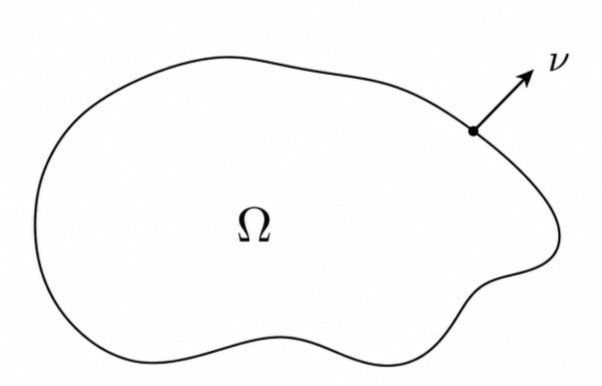
\includegraphics[width=0.6\linewidth]{pics/4.png}
        \caption{Область $\Omega$ и нормаль $\nu$}
        \label{fig:enter-label}
\end{figure}
Начально краевая задача:
\[\begin{cases}
    \dfrac{\partial U}{\partial t} - \LL U = f \\
    U\big|_{t=t_0}=U_0 
    \end{cases} \quad 
    \begin{cases}
        \dfrac{\partial^2 U}{\partial t^2} - \LL U = f \\
        U\big|_{t=0}=U_0, \,\,\, \dfrac{\partial U}{\partial t}\bigg|_{t=0}=U_2
    \end{cases}\]
И еще одно условие на на краевые условия. Мы хотим чтобы решение существовало, чтобы оно было единственным и чтобы устойчивым (непрерывно зависит от данных задачи).
\begin{myexample}
Пример Адамара: 
$$\dfrac{\partial^2 U}{\partial x^2}+\dfrac{\partial^2 U}{\partial x^2}=0, \quad (x,y)\in\R^2, y>0$$
$$U\big|_{y=0}=\phi, \,\,\,\, \dfrac{\partial U}{\partial y}\bigg|_{y=0}=0$$
Возьмём такие $\phi_m$: $\,\,\, \phi_m(x)=e^{-\sqrt{m}}\cos mx, \quad \phi_m\xrightarrow[m\to\infty]{}0$ \\
Возьмём следующее решение: $U_m(x,y)=e^{-\sqrt{m}}\cos mx\cosh my$. Посмотрим на точку с координатами $(0, \epsilon)$ и получим: 
\[U_m(0, \epsilon)=e^{-\sqrt{m}}\big(\dfrac{e^{m\epsilon}+e^{-m\epsilon}}{2}\big)\xrightarrow[m\to\infty]{}\infty\]
Здесь как бы нету непрерывности, ведь краевые условия стремятся к 0, а решение к бесконечности.
\end{myexample}
\section{Одномерное волновое уравнение}
\subsection{Уравнение струны}
\begin{tikzpicture}[>=stealth, scale=1.2]


\draw[->] (-0.2,0) -- (7.2,0) node[right] {$x$};
\draw[->] (0,-1.2) -- (0,2.0) node[above] {$U(t,x)$};


\draw[thick, smooth] 
  plot coordinates {
    (-0.1,0.15)
    (0.8,-0.18)
    (1.8,-0.28)
    (2.8,0.10)
    (3.8,0.78)
    (4.6,0.98)
    (5.6,0.78)
    (6.8,0.18)
  };


\draw (4.00,0.06) -- (4.00,-0.06);
\draw (4.85,0.06) -- (4.85,-0.06);
\node[below] at (4.00,-0.06) {$x_0$};
\node[below] at (4.85,-0.06) {$x_0+dx$};


\coordinate (P0) at (4.10,0.90);
\coordinate (P1) at (4.85,0.90);
\fill (P0) circle (1.2pt);
\fill (P1) circle (1.2pt);


\draw[thin] ($(P0)+(-0.65,0)$) -- ($(P0)+(0.65,0)$);
\draw[thin] ($(P1)+(-0.65,0)$) -- ($(P1)+(0.65,0)$);
\draw[->, thick] (P0) -- ++(-1.05,-0.28) node[above left] {$\vec{T}_0$};
\draw[->, thick] (P1) -- ++(1.10,-0.10) node[above right] {$\vec{T}_1$};
\draw[line width=0.9pt] (P0) ++(180:0.42) arc[start angle=180,end angle=195,radius=0.42];
\node at ($(P0)+(-0.55,-0.18)$) {$\alpha_0$};

\draw[line width=0.9pt] (P1) ++(0:0.42) arc[start angle=0,end angle=-5,radius=0.42];
\node at ($(P1)+(0.52,-0.14)$) {$\alpha_1$};

\end{tikzpicture}\\
$\vec{T_0}+\vec{T_1}=m\vec{a}, \quad m=\rho\dd x$ \\
Примем, что $|T_0|=|T_1|=T$. Тогда:
$$-T\sin\alpha+0+T\sin\alpha_1=\rho \dd x \dfrac{\partial^2 U(t,x)}{\partial t^2}$$
Прибегая к малости углов ($\sin\alpha\approx\tan\alpha$):
\[\begin{aligned}\sin\alpha_0\approx\dfrac{\partial U(t, x_0)}{\partial x}\\
\sin\alpha_1\approx\dfrac{\partial U(t, x_0+\dd x)}{\partial x}\end{aligned} \quad \Rightarrow \quad \sin\alpha_1-\sin\alpha_0=\dfrac{\partial^2 U(t,x_0)}{\partial x^2}\dd x\]
Получим знакомое волновое уравнение: 
\[T\dfrac{\partial^2 U}{\partial x^2}\dd x=\rho \dd x\dfrac{\partial^2 U}{\partial t^2} \quad \Leftrightarrow \quad \dfrac{\partial^2 U}{\partial^2 t}-c^2\dfrac{\partial^2 U}{\partial x^2}=0, \,\,\, c=\sqrt{\dfrac{T}{\rho}}\]
1) бесконечная длина: 
\lbpn{volna}{ \[ \begin{cases}
    \dfrac{\partial^2 U}{\partial^2 t}-c^2\dfrac{\partial^2 U}{\partial x^2}=0, \,\,\, t\geq0, x\in\R \\
    U\big|_{t=0}=\phi(x), \,\,\, \dfrac{\partial U}{\partial t}\bigg|_{t=0}=\psi(x)
 \end{cases}\]}
Вот такую задачу мы хотим решать.


\subsection{Метод Даламбера}
Введём следующие переменные: \[\xi\coloneqq x+ct \qquad \eta\coloneqq x-ct \]
Тогда: \[x=\dfrac{\xi+\eta}{2} \qquad t=\dfrac{\xi-\eta}{2c}\]
Тогда производные по новым переменным: 
\[\dfrac{\partial}{\partial \xi}=\dfrac{\partial x}{\partial \xi}\dfrac{\partial}{\partial x}+\dfrac{\partial t}{\partial \xi}\dfrac{\partial}{\partial t}=\dfrac{1}{2}\dfrac{\partial}{\partial x}+\dfrac{1}{2c}\dfrac{\partial}{\partial t}\]
\[\dfrac{\partial}{\partial \eta}=\dfrac{1}{2}\dfrac{\partial}{\partial x}-\dfrac{1}{2c}\dfrac{\partial}{\partial t}\]
\[\dfrac{\partial^2 U}{\partial \xi \partial \eta}=\bigg(\dfrac{1}{2}\dfrac{\partial}{\partial x}+\dfrac{1}{2c}\dfrac{\partial}{\partial t}\bigg)\bigg(\dfrac{1}{2}\dfrac{\partial}{\partial x}+\dfrac{1}{2c}\dfrac{\partial}{\partial t}\bigg)U(t,x)=\dfrac{1}{4}\bigg(\dfrac{\partial^2 U}{\partial x^2}-\dfrac{1}{c^2}\dfrac{\partial^2 U}{\partial t^2}\bigg)\]
То есть $\bigg(\dfrac{\partial^2 U}{\partial x^2}-\dfrac{1}{c^2}\dfrac{\partial^2 U}{\partial t^2}\bigg)=0$ равносильно $\dfrac{\partial^2 U}{\partial \xi \partial \eta}=0$. Значит:
\[\dfrac{\partial }{\partial \xi}\bigg(\dfrac{\partial U}{\partial \eta}\bigg)=0 \quad \Rightarrow \quad \dfrac{\partial U}{\partial \eta}=const_\xi=\alpha(\eta)\]
Тогда \(U=\int\limits_{0}^{\eta}\alpha(\tau)\dd \tau + c(\xi)\)
Аналогичные рассуждения и для $\xi$. Тогда получим, что 
\[\dfrac{\partial^2 U}{\partial \xi\partial \eta}=0 \quad \Leftrightarrow \quad U=f(\xi)+g(\eta)\]
Тогда получаем известное решение волнового уравнения: 
\lbpn{volnasol}{\[U(t,x)=f(x+ct)+g(x-ct)\]}
Это утверждение работает в любых классах. \\
Разберемся теперь с начальными условиями: 
\[t=0: \begin{cases}
    f(x)+g(x)=\phi(x) \\
    cf'(x)-cg'(x)=\psi(x)
\end{cases} \quad \Rightarrow \quad \begin{cases}
    f'(x)+g'(x)=\phi'(x) \\
    f'(x)-g'(x)=\dfrac{1}{c}\psi(x)
\end{cases}\]
\(\begin{cases}
    f'(x)=\dfrac{1}{2}\bigg(\phi'(x)+\dfrac{1}{c}\psi(x)\bigg) \\
    g'(x)=\dfrac{1}{2}\bigg(\phi'(x)-\dfrac{1}{c}\psi(x)\bigg)
\end{cases}\) \\
\(\begin{cases}
    f(x)=\dfrac{\phi(x)}{2}+\dfrac{1}{2c}\int\limits_{0}^{x}\psi(y)\dd y+A_1 \\
    f(x)=\dfrac{\phi(x)}{2}-\dfrac{1}{2c}\int\limits_{0}^{x}\psi(y)\dd y+A_2
\end{cases} \qquad f(x)+g(x)=\phi(x) \quad \Rightarrow \quad A_1+A_2=0\)
Тогда получаем следующее решение из \ref{volnasol}: 
\[U(t,x)=\dfrac{\phi(x+ct)+\phi(x-ct)}{2}+\dfrac{1}{2c}\int\limits_{x-ct}^{x+ct}\psi(y)\dd y - \text{ формула Даламбера}\]
\begin{mytheorem}
    \lbpn{true}{Пусть \(\phi\in\C^2(\R), \,\,\psi\in\C(\R) \quad \Rightarrow \quad \exists! \,\,\, U\in\C^2([0, +\infty)\times R)\) - решения задачи \ref{volna} и формула Даламбера явялется выражением для него}
\end{mytheorem}
Свойства решения: \\
1) Пусть $\psi\equiv0$: 
\begin{figure}[H]
        \centering
        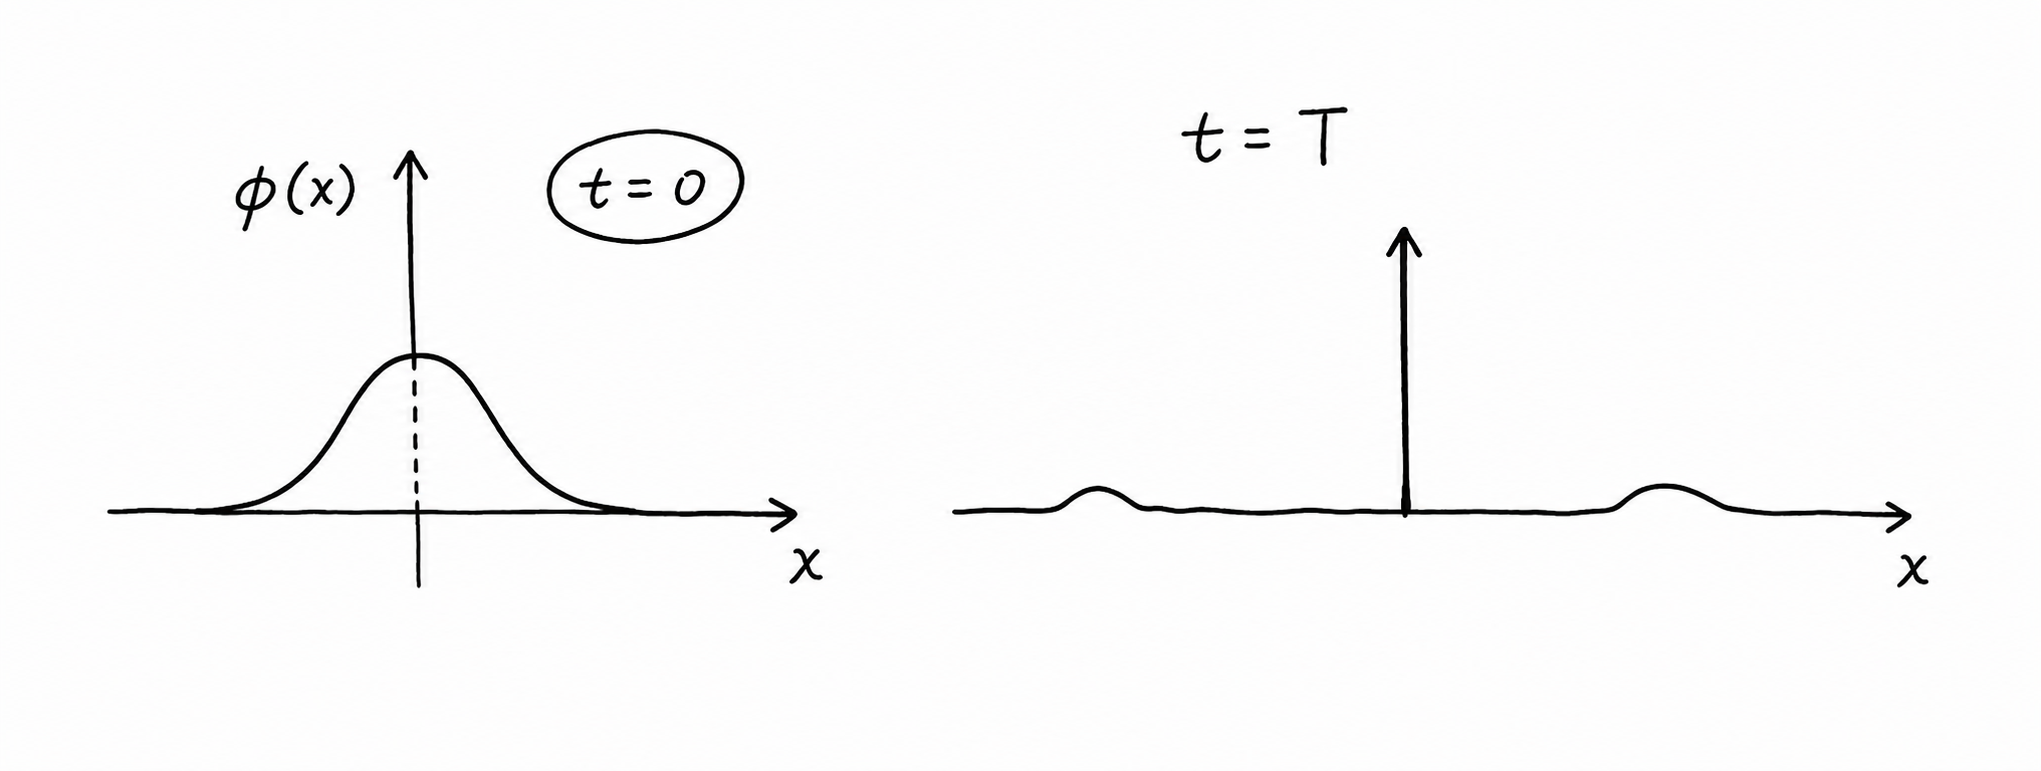
\includegraphics[width=0.6\linewidth]{pics/5.png}
        \caption{}
        \label{fig:enter-label}
\end{figure} 
Здесь на кртинке пики как бы смещаются на $ct$ влево и вправо и еще в 2 рааз уменьшаются.\\
$\supp \phi\subset[a, b]$
\begin{figure}[H]
        \centering
        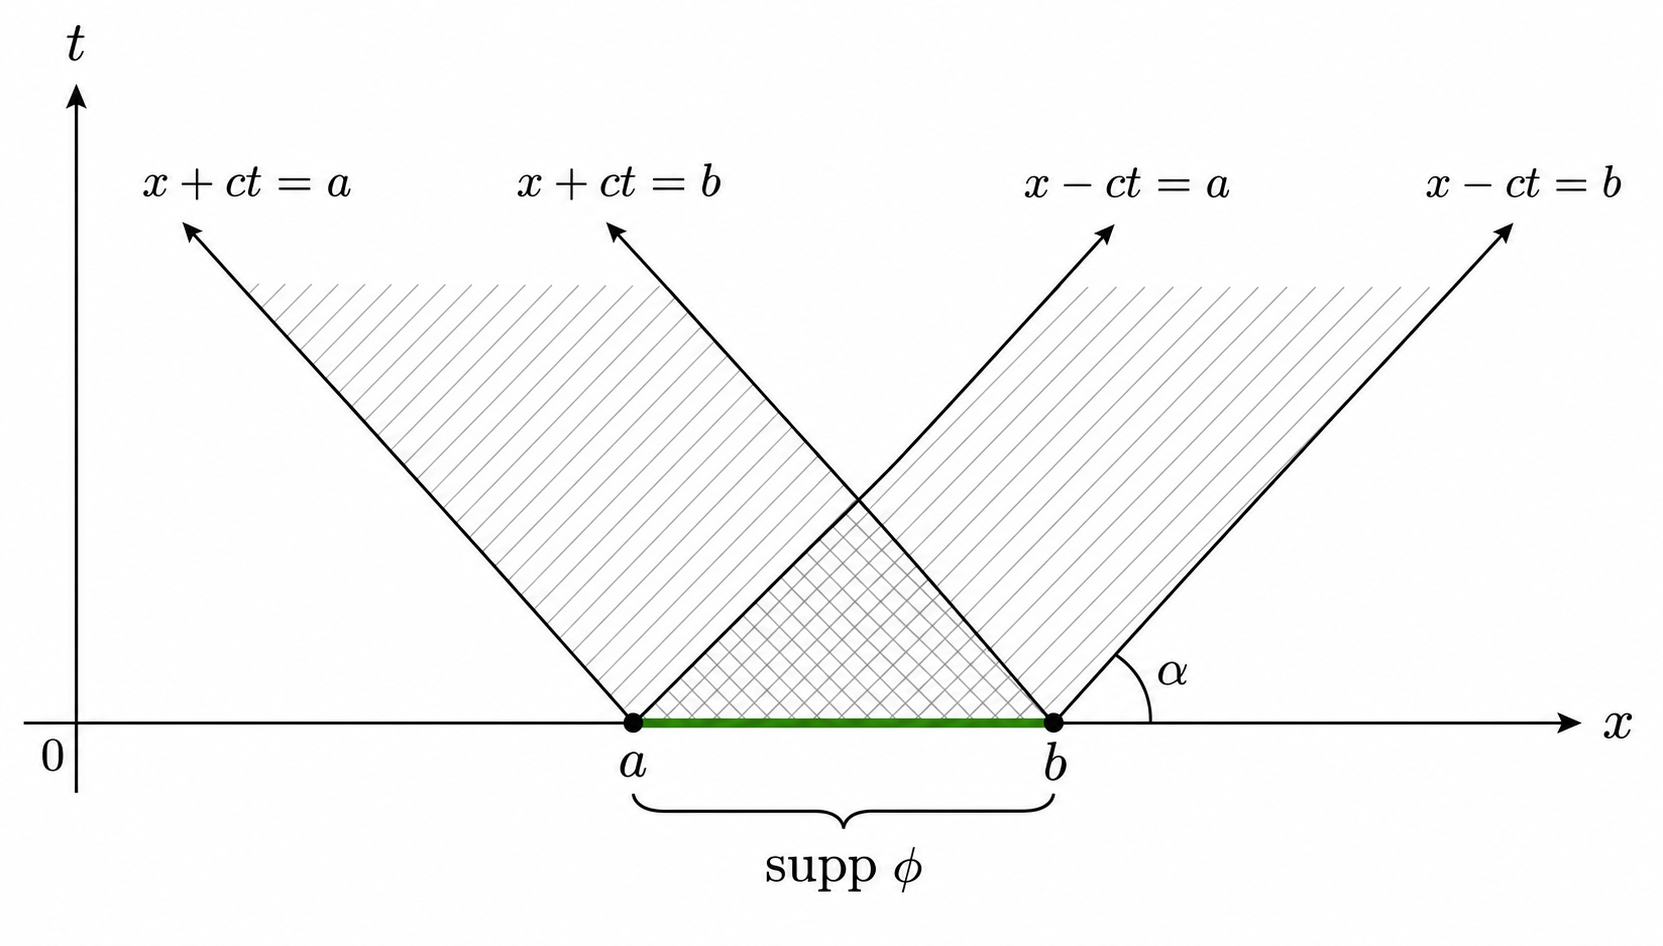
\includegraphics[width=0.6\linewidth]{pics/6.png}
        \caption{}
        \label{fig:enter-label}
\end{figure}
На рисунке показан как раз $\supp U$, если провести вертикальную линию при постоянном $x$ то мы получим как раз что-то типо профиля волны, которая убегает на бесконечность, $\tan\alpha=\dfrac{1}{c}$\\
2) Пусть $\phi, \psi - \forall$ 
\begin{figure}[H]
        \centering
        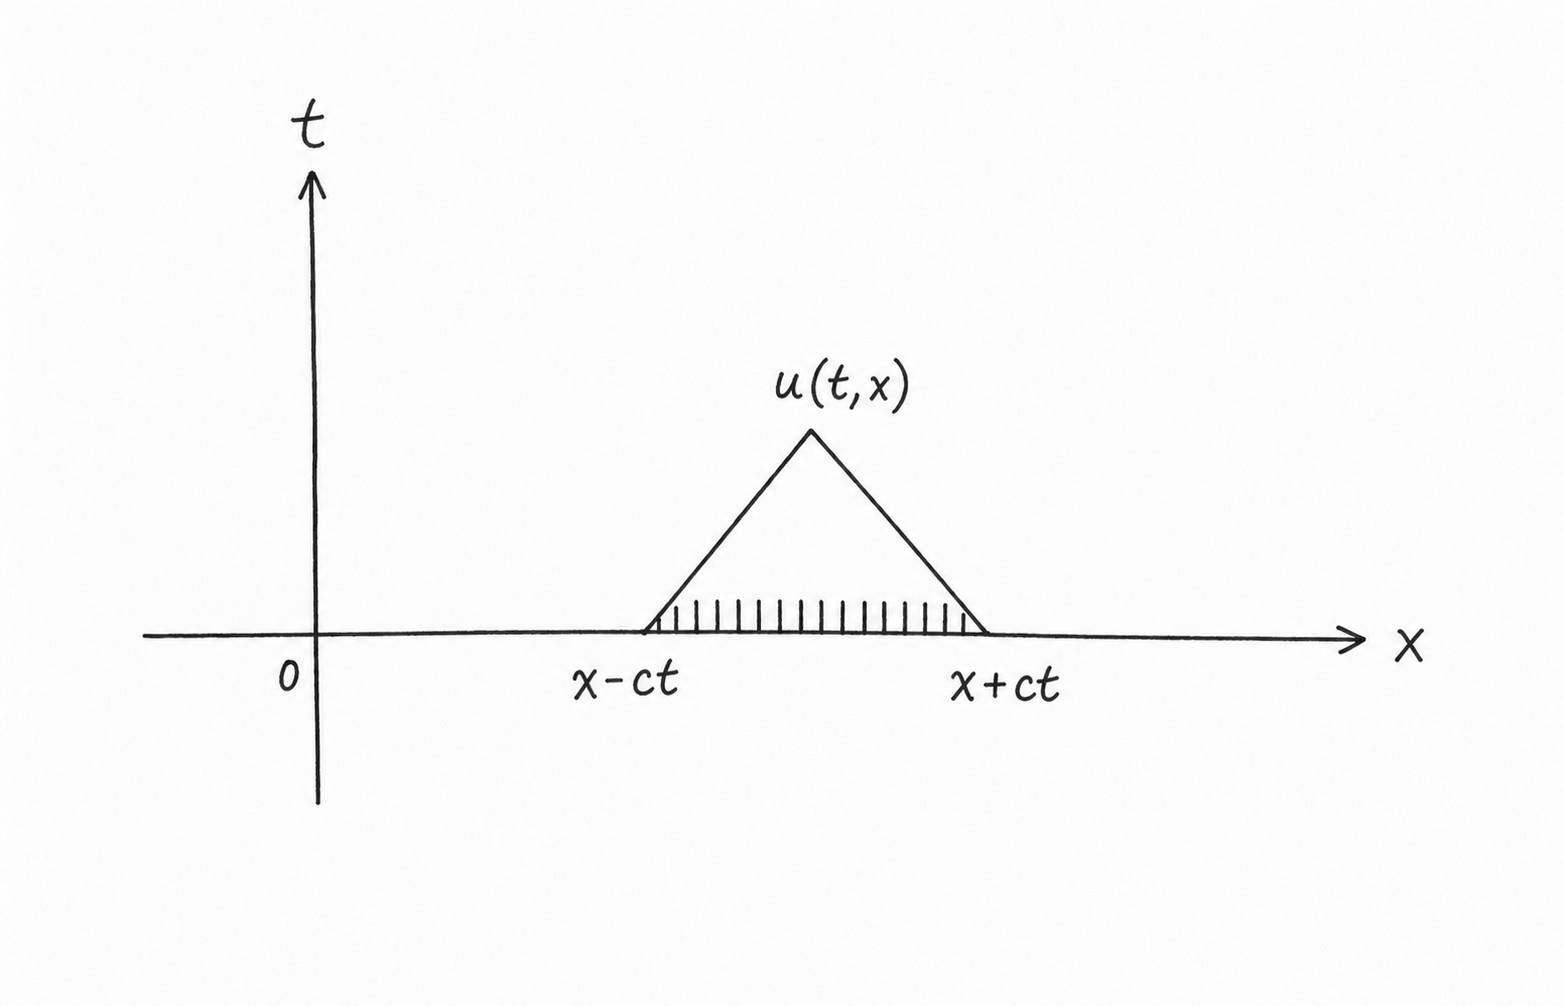
\includegraphics[width=0.6\linewidth]{pics/7.png}
        \caption{}
        \label{fig:enter-label}
\end{figure}

На решение $U(t,x)$ влияет только то, что находится на заштрихованной оси, а от другой части информация в эту точку не приходит.
\subsection{Функция Грина для бесконечной струны}
Возьмём следующую обобщённуйю функцию, которая по одной переменной бесконечно гладкая, а по другой является обобщённой функцией:
\[g(t, x) \quad g\in\Cinf((0,\infty), \DDR)\]
Пусть $\phi\in\DR$: \\
$\exists \dfrac{\dd}{\dd t}\big(g(t, \cdot), \phi\big)$ - тоже обобщённая функция. \\
\[\dfrac{\dd}{\dd t}\big(g(t, \cdot), \phi\big)=\bigg(\dfrac{\partial g}{\partial t}(t, \cdot), \phi\bigg)\]
$\forall \phi\in\DR \quad \forall m\in\N$
\[\exists \dfrac{\dd^m}{\dd t^m}\big(g(t,\cdot), \phi\big)=\bigg(\dfrac{\partial^m g(t,\cdot)}{\partial t^m}, \phi\bigg) \quad \dfrac{\partial^m g}{\partial t^m}\in\DDR\]
\begin{mydef}
    $g$ - функция Грина для уравнения струны $\quad\Leftrightarrow$ 
    \lbpn{gvolna}{\[\Leftrightarrow \quad g\in\Cinf((0,\infty), \DDR) \text{ и }\begin{cases}
        \dfrac{\partial^2 g(t, x)}{\partial t^2} - c^2\dfrac{\partial^2 g(t,x)}{\partial x^2}=0 \\
        g\xrightarrow[t\to0]{\DDR}0, \quad \dfrac{\partial g}{\partial t}\xrightarrow[t\to0]{\DDR}\delta(x)
    \end{cases}\]}
Важно что производная по $x$ берётся как производная обобщённой функции.
\end{mydef}
Используем формулу Даламбера из предыдущего параграфа и подставим туда $0, \delta(x)$ вместо $\phi, \psi$:
\[g(t,x)=\dfrac{1}{2с}\int\limits_{x-ct}^{x+ct}\delta(y)\dd y\]
Но это определение некорректно и так писать нельзя, но 'мы с вами физики' поэтому определим просто вот так:
\[g(t,x)=
\left[
\begin{array}{l}
\dfrac{1}{2c}, \quad |x|<ct \\
0, \quad |x|>ct
\end{array}
\right.
\]
Для фиксированного $t$ график выглядит вот так:
\begin{figure}[H]
        \centering
        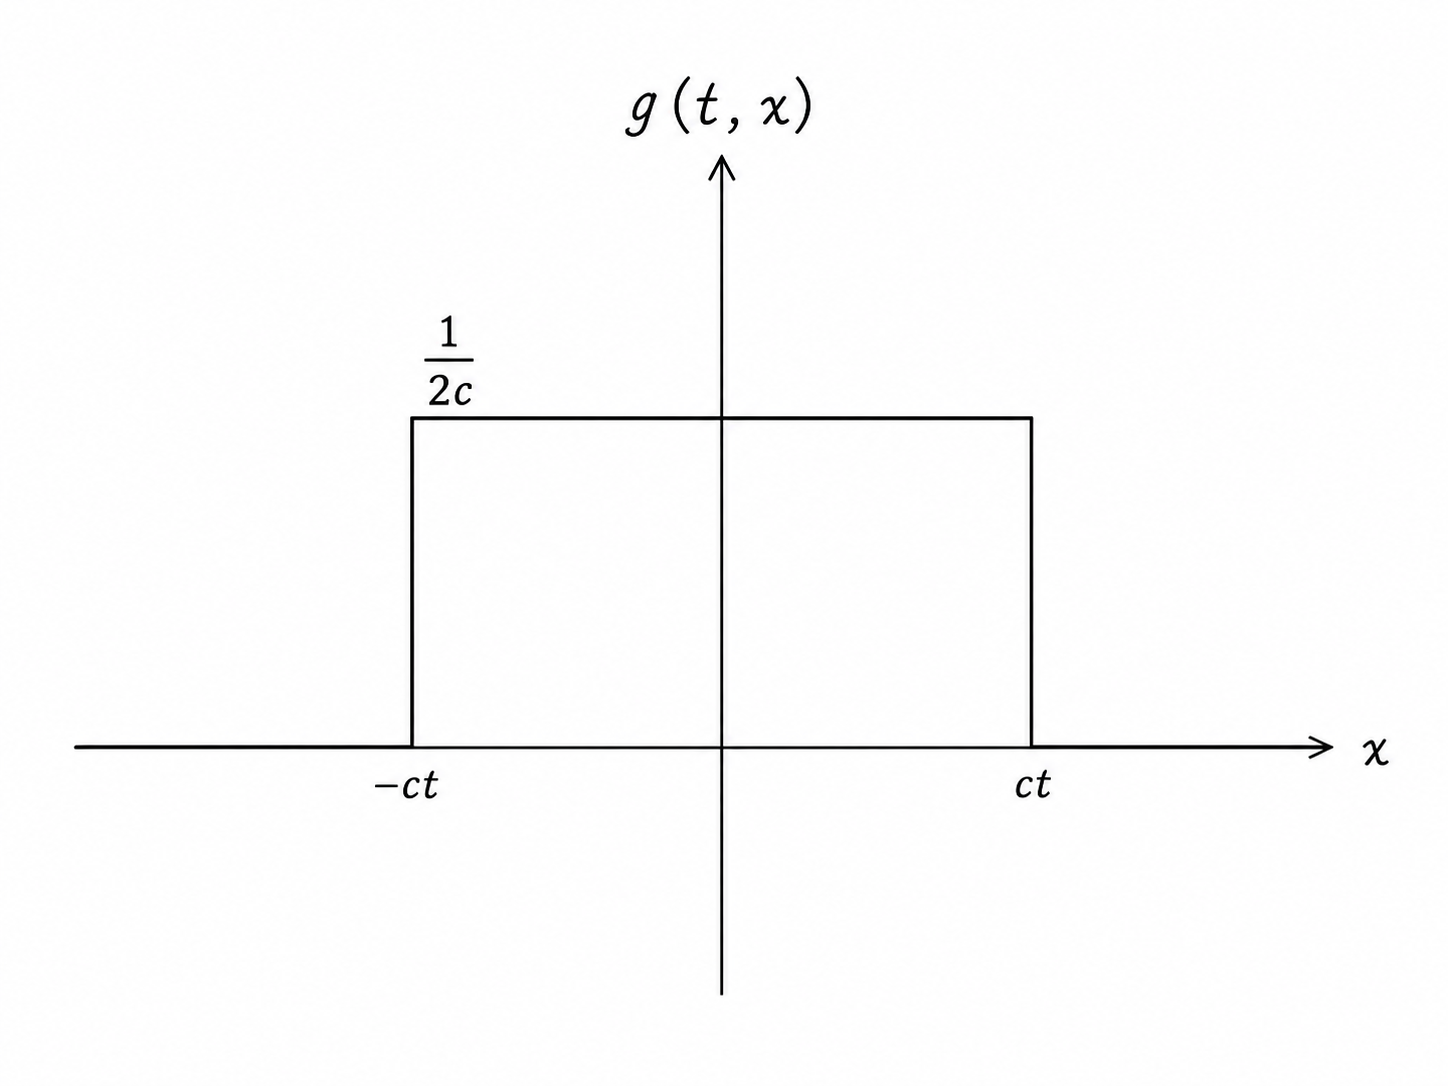
\includegraphics[width=0.6\linewidth]{pics/8.png}
        \caption{}
        \label{fig:enter-label}
\end{figure}

Заметим, что $g$ - обобщённая функция, действие которой определяется как:
\[\big(g(t, \cdot), \phi\big)=\dfrac{1}{2c}\int\limits_{-ct}^{ct}\phi(x)\dd x\]
Пусть $\phi\in\DR$, тогда по свойству дифференцирования переменного предела:
\[\exists \dfrac{\dd}{\dd t}\bigg(g(t,\cdot), \phi\bigg)=\dfrac{1}{2}\phi(ct)+\dfrac{1}{2}\phi(-ct)\]
\[\exists \dfrac{\dd^2}{\dd t^2}\bigg(g(t,\cdot), \phi\bigg)=\dfrac{c}{2}\phi'(ct)-\dfrac{c}{2}\phi'(-ct)\]
Заметим, что \(\int\limits_{-ct}^{ct}\phi(x)\dd x\leftrightarrow(\theta(x+ct)-\theta(x-ct), \phi)\), \(\quad \phi(ct)\leftrightarrow(\delta(x-ct), \phi(x))\), \(\quad \phi'(ct)\leftrightarrow(-\delta'(x-ct),\phi)\). Тогда это все переписывается вот так:
\[g(t,x)=\dfrac{1}{2c}\bigg(\theta(x+ct)-\theta(x-ct)\bigg)\]
\[\dfrac{\partial g}{\partial t}(t,x)=\dfrac{1}{2}\bigg(\delta(x+ct)-\delta(x-ct)\bigg)\]
\[\dfrac{\partial^2 g}{\partial t^2}(t,x)=\dfrac{c}{2}\bigg(\delta'(x+ct)-\delta'(x-ct)\bigg)\]
\[\dfrac{\partial g}{\partial x}(t, x)=\dfrac{1}{2c}\bigg(\delta(x+ct)-\delta(x-ct)\bigg)\]
\[\dfrac{\partial^2 g}{\partial x^2}(t, x)=\dfrac{1}{2c}\bigg(\delta'(x+ct)-\delta'(x-ct)\bigg)\]
Отсюда видно, что волновое уравнение \ref{gvolna} выполняется. \\
Теперь посмотрим на граничные условия: 
\[\big(g(t, \cdot), \phi\big)\overset{\forall \phi\in\DR}{=}\dfrac{1}{2c}\int\limits_{-ct}^{ct}\phi(x)\dd x\xrightarrow[t\to0]{}0\]
\[\bigg(\dfrac{\partial g}{\partial t}(t, \cdot), \phi\bigg)=\dfrac{1}{2}\big(\phi(ct)+\phi(-ct)\big)\xrightarrow[t\to0]{}\phi(0)=(\delta,\phi)\]
Теперь возьмём 'похожую' функцию, которая уже будет обобщённой по обеим переменным: $G\in\D'(\R^2)$ \\

\[G(t, x)=\left[
\begin{array}{l}
\dfrac{1}{2c}, \quad \begin{aligned}
    t>0 \\
    |x|<ct
\end{aligned} \\
0, \quad \text{иначе}
\end{array}
\right.\]
\begin{figure}[H]
        \centering
        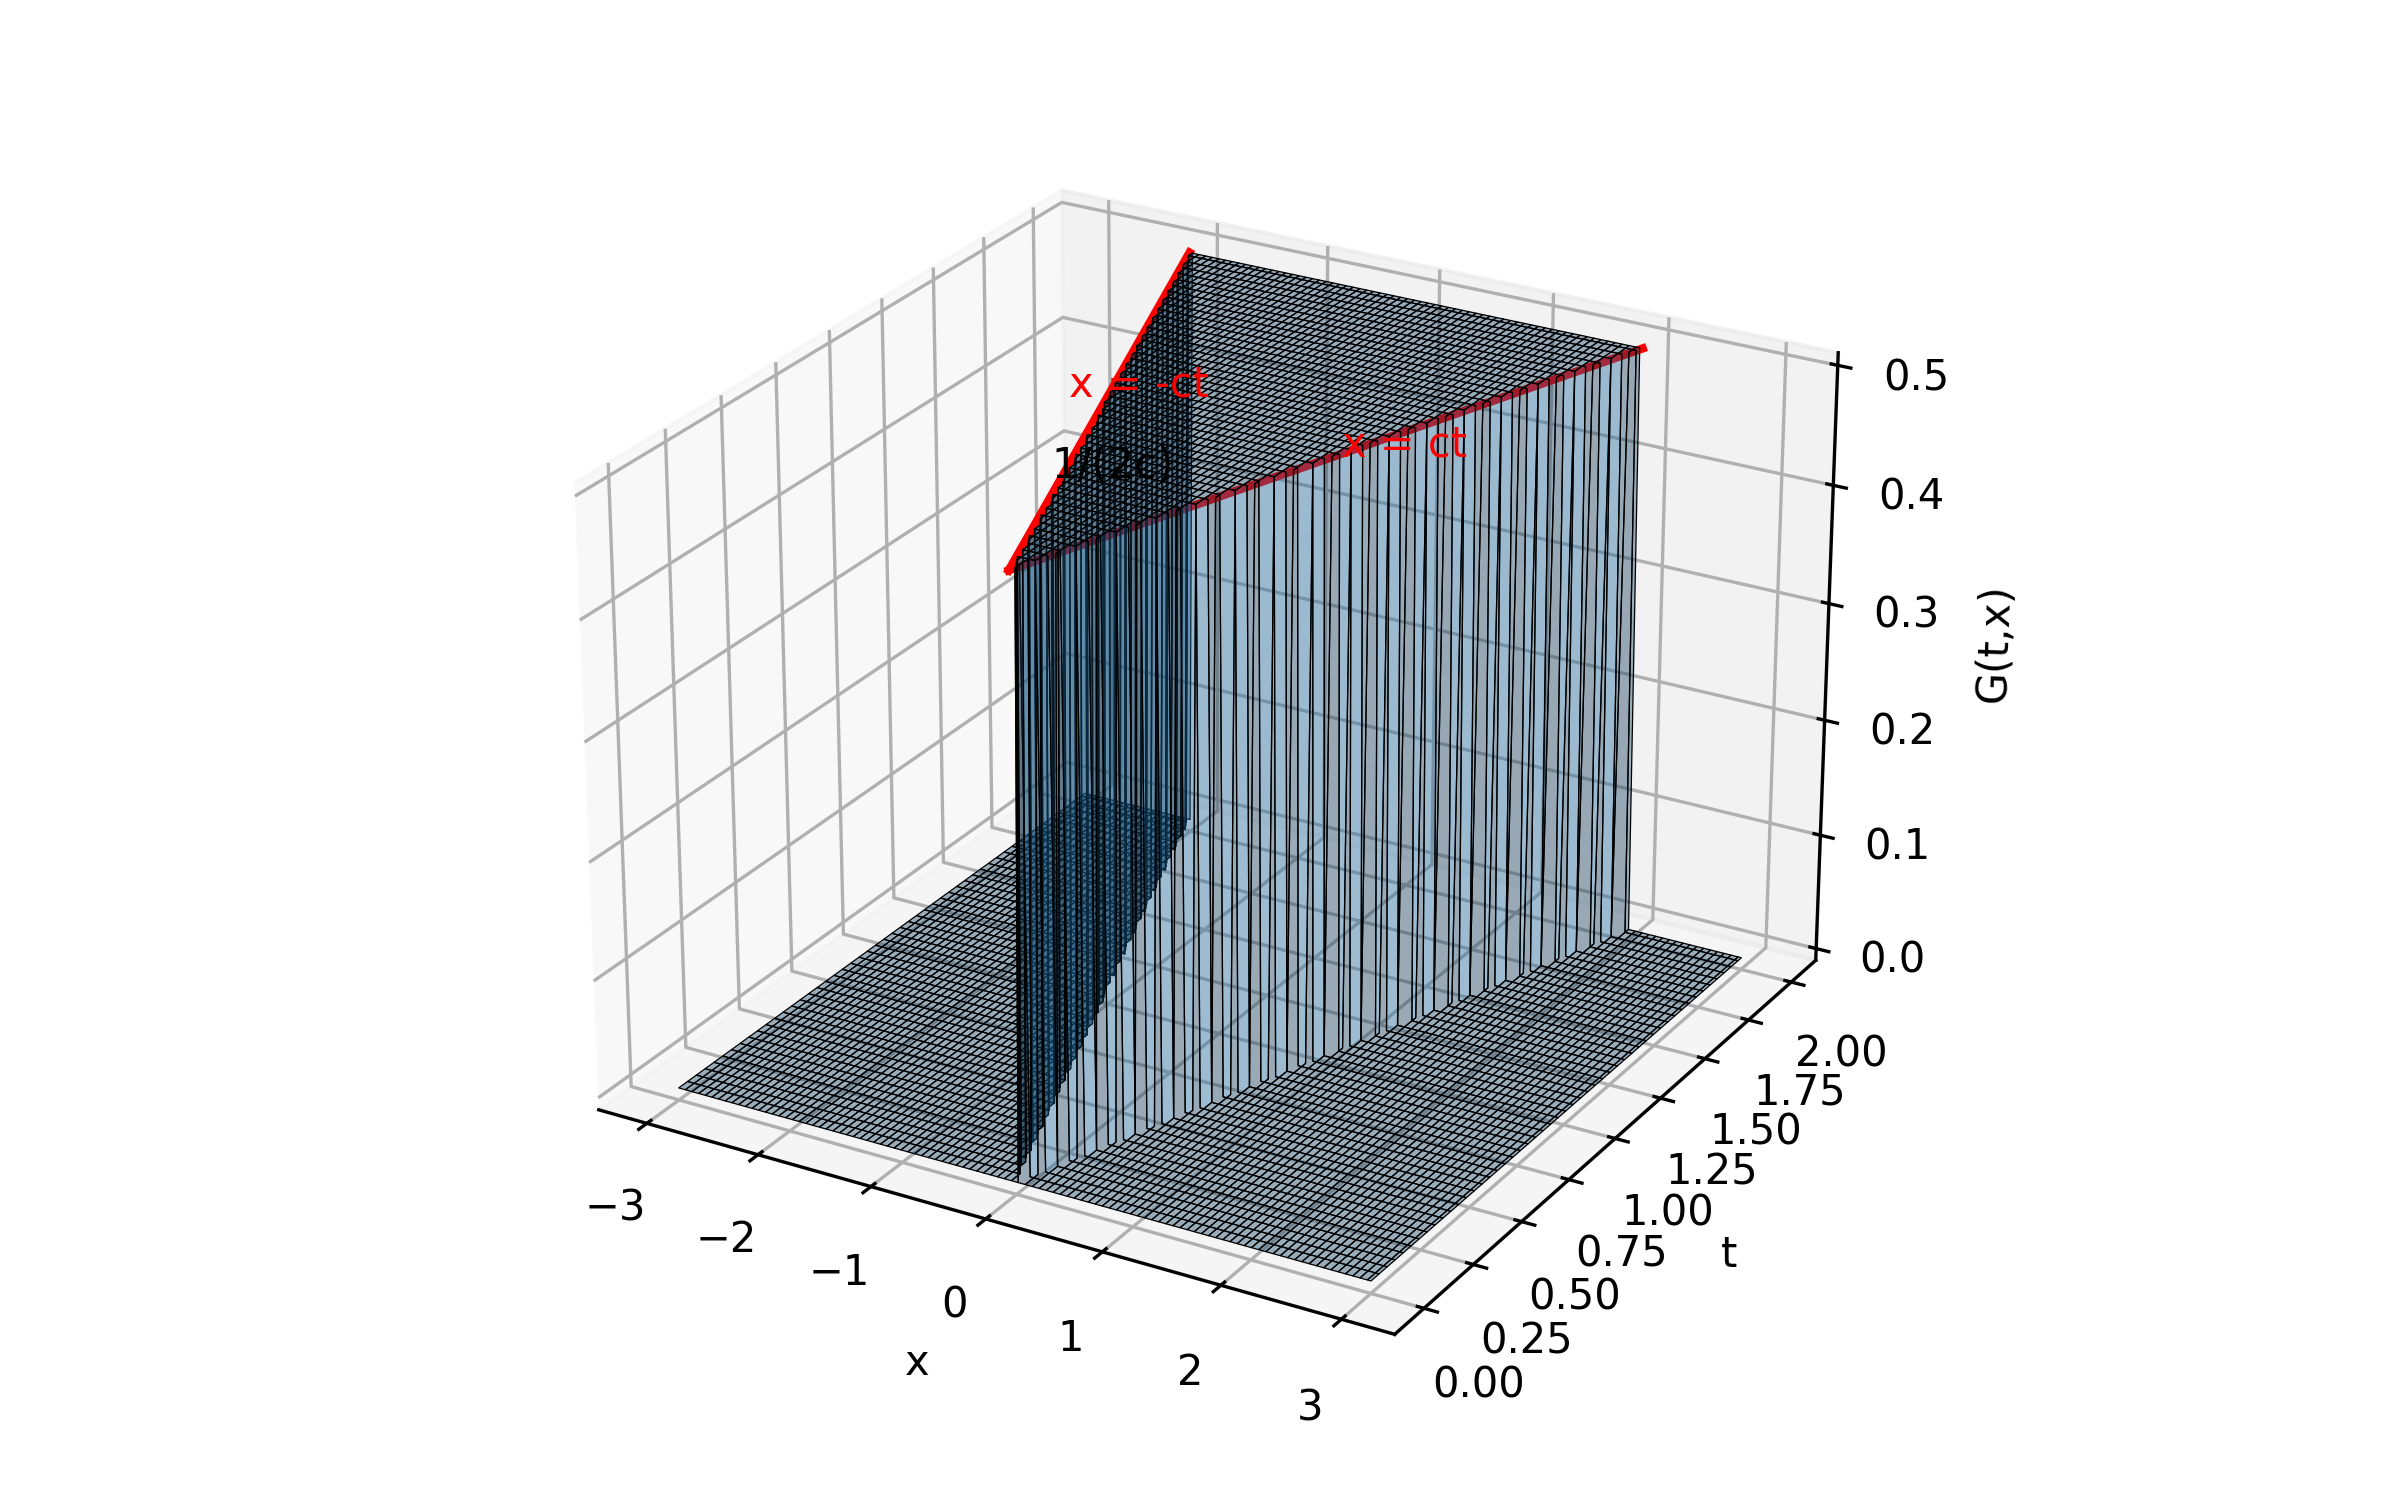
\includegraphics[width=0.6\linewidth]{pics/9.png}
        \caption{}
        \label{fig:enter-label}
\end{figure}

\begin{myexe}
    \lbpn{lol}{\[\dfrac{\partial^2 G}{\partial t^2}-c^2\dfrac{\partial^2 G}{\partial x^2}=\delta(t, x)\]}
Пусть
\[
G(t,x)=\frac{1}{2c}\,\theta(t)\bigl(\theta(x+ct)-\theta(x-ct)\bigr).
\]


\[
\frac{\partial G}{\partial x}=\frac{1}{2c}\,\theta(t)\bigl(\delta(x+ct)-\delta(x-ct)\bigr),
\]
\[
\frac{\partial^{2} G}{\partial x^{2}}=\frac{1}{2c}\,\theta(t)\bigl(\delta'(x+ct)-\delta'(x-ct)\bigr).
\]


\[
\frac{\partial G}{\partial t}=
\frac{1}{2c}\,\delta(t)\bigl(\theta(x+ct)-\theta(x-ct)\bigr)
+\frac{1}{2}\,\theta(t)\bigl(\delta(x+ct)+\delta(x-ct)\bigr).
\]

\[
\frac{\partial^{2} G}{\partial t^{2}}=
\frac{1}{2c}\,\delta'(t)\bigl(\theta(x+ct)-\theta(x-ct)\bigr)
+\delta(t)\bigl(\delta(x+ct)+\delta(x-ct)\bigr)
+\frac{c}{2}\,\theta(t)\bigl(\delta'(x+ct)-\delta'(x-ct)\bigr).
\]


\[
\square G=\frac{\partial^{2}G}{\partial t^{2}}-c^{2}\frac{\partial^{2}G}{\partial x^{2}}.
\]
Слагаемые с $\theta(t)\delta'$ сокращаются:
\[
\frac{c}{2}\,\theta(t)(\delta'(x+ct)-\delta'(x-ct))-c^{2}\cdot\frac{1}{2c}\,\theta(t)(\delta'(x+ct)-\delta'(x-ct))=0.
\]
Остаётся
\[
\square G=
\frac{1}{2c}\,\delta'(t)\bigl(\theta(x+ct)-\theta(x-ct)\bigr)
+\delta(t)\bigl(\delta(x+ct)+\delta(x-ct)\bigr).
\]


\[
\langle\square G,\varphi\rangle=
\frac{1}{2c}
\iint\delta'(t)\bigl(\theta(x+ct)-\theta(x-ct)\bigr)\varphi(t,x)\,dt\,dx
+\iint\delta(t)\bigl(\delta(x+ct)+\delta(x-ct)\bigr)\varphi(t,x)\,dt\,dx.
\]

Первый интеграл:
\[
\frac{1}{2c}\iint\delta'(t)\Phi(t,x)\,dt\,dx
=-\frac{1}{2c}\iint\delta(t)\frac{\partial\Phi}{\partial t}(t,x)\,dt\,dx,
\]
где $\Phi(t,x)=(\theta(x+ct)-\theta(x-ct))\varphi(t,x)$. 


Вычисляем производную $\Phi$ по $t$:
\[
\frac{\partial\Phi}{\partial t}=
\bigl(c\delta(x+ct)+c\delta(x-ct)\bigr)\varphi(t,x)
+\bigl(\theta(x+ct)-\theta(x-ct)\bigr)\frac{\partial\varphi}{\partial t}(t,x).
\]
При $t=0$:
\[
\theta(x+0)-\theta(x-0)=\theta(x)-\theta(x)=0,
\]
\[
\delta(x+c\cdot0)=\delta(x),\qquad
\delta(x-c\cdot0)=\delta(x).
\]
Следовательно,
\[
\frac{\partial\Phi}{\partial t}\big|_{t=0}=
\bigl(c\delta(x)+c\delta(x)\bigr)\varphi(0,x)=2c\,\delta(x)\,\varphi(0,x).
\]


\[
-\frac{1}{2c}\iint\delta(t)\frac{\partial\Phi}{\partial t}(t,x)\,dt\,dx
=-\frac{1}{2c}\int_{-\infty}^{\infty}\left(2c\,\delta(x)\varphi(0,x)\right)dx
=-\int_{-\infty}^{\infty}\delta(x)\varphi(0,x)dx=-\varphi(0,0).
\]

\[
\iint\delta(t)\bigl(\delta(x+ct)+\delta(x-ct)\bigr)\varphi(t,x)\,dt\,dx
=\int_{-\infty}^{\infty}\bigl(\delta(x)+\delta(x)\bigr)\varphi(0,x)dx=2\varphi(0,0).
\]


\[
\langle\square G,\varphi\rangle=-\varphi(0,0)+2\varphi(0,0)=\varphi(0,0),
\]
что соответсвует $\delta(t, x)$
\end{myexe}



\begin{mydef}
    $G$ - фундаментальное решение уравнения струны $\quad \Leftrightarrow$ 
    \[\Leftrightarrow \quad G\in\D'(\R^2) \text{ и }\begin{cases}
        \dfrac{\partial^2 G}{\partial t^2}-c^2\dfrac{\partial^2 G}{\partial x^2}=\delta(t, x) \\
        G\big|_{t<0}=0
    \end{cases}\]
\end{mydef}
Нужно проверить, что $\forall \phi\in\D(\R^2)$(кажется это следует из \ref{lol}):
\[\int\limits_{\R^2}G(t,x)\bigg(\dfrac{\partial^2 \phi(t,x)}{\partial t^2}-c^2\dfrac{\partial^2 \phi(t,x)}{\partial x^2}\bigg)\dd x\dd t=\phi(0,0)\]
Иногда пишут, что \(G(t,x)=g(t,x)\theta(t)\), но это не очень корректная запись.
\begin{myremark}
    В книжках слова фундаментальное решение и функция Грина это синонимы.
\end{myremark}
Хотим решить ($\LL$ - дифференциальный оператор):
\[\LL U = f \]
Для решения такой задачи сначала ищем фундаментальное решение: \(\LL G=\delta\), а затем делаем свёртку: $U=G\ast f$. \\
Проверка: \(\LL U=\LL(G\ast f)=\LL G \ast f=\delta\ast f=f\)\\
Тут мы использовали тот факт, что производные в свёртке можно кидать на любой множитель. \\
\begin{mytheorem}
    Пусть \(\phi\in\C^2(\R), \psi\in\C^1(\R), f\in\C^1([0,\infty)\times\R)\)
    \[\exists! U\in\C^2([0,\infty)\times\R):\begin{cases}
        \dfrac{\partial^2 U}{\partial t^2}-c^2\dfrac{\partial^2 U}{\partial x^2}=f, \quad t\geq0, x\in\R \\
        U\big|_{t=0}=\phi(x), \quad \dfrac{\partial U}{\partial t}\bigg|_{t=0}=\psi(x)
    \end{cases}\]
    \[U=\dfrac{\partial g}{\partial t}\ast\phi+g\ast\psi+G\ast f=\]
    \[=\int\limits_\R \dfrac{\partial g}{\partial t}(t, x-y)\phi(y)\dd y+\int\limits_\R g(t, x-y)\psi(y)\dd y+\int\limits_{0}^{t}\int\limits_\R g(t-\tau, x-y)f(\tau, y)\dd y\dd \tau=U_1+U_2+U_3\]
\end{mytheorem}
\begin{myproof}
   Знаем: \(\dfrac{\partial g}{\partial t}=\dfrac{1}{2}\big(\delta(x+ct)+\delta(x-ct)\big)\). \\
   1) \[U_1(t,x)=\dfrac{1}{2}\int\limits_{R}\big(\delta(x-y+ct)+\delta(x-y-ct)\big)\phi(y)\dd y=\dfrac{1}{2}\big(\phi(x+ct)-\phi(x-ct)\big) \quad \Rightarrow\]
   \[\Rightarrow \quad \begin{cases}
    \dfrac{\partial^2 U_1}{\partial t^2}-c^2\dfrac{\partial^2 U_1}{\partial x^2}=0 \\
    U_1(t=0)=\phi(x), \quad \dfrac{\partial U_1}{\partial t}\bigg|_{t=0}=0
   \end{cases}\]
   2) \[U_2(t, x)=\int\limits_\R \dfrac{1}{2c}\underbrace{\chi_{[-ct; ct]}(x-y)}_\text{характер. функция}\psi(y)\dd y=\dfrac{1}{2c}\int\limits_{x-ct}^{x+ct}\psi(y)\dd y \quad \Rightarrow\]
   \[\Rightarrow \quad \begin{cases}
    \dfrac{\partial^2 U_2}{\partial t^2}-c^2\dfrac{\partial^2 U_2}{\partial x^2}=0 \\
    U_2(t=0)=0, \quad \dfrac{\partial U_2}{\partial t}\bigg|_{t=0}=\psi(x)
   \end{cases}\]
   \[(U_1+U_2)\text{ - формула Даламбера}\]
   И мы получили решение для нулевой правой части волнового уравнения. Теперь остаётся только $U_3$. \\
   3) \[U_3(t, x)=\int\limits_{0}^{t}\int\limits_\R g(t-\tau, x-y)f(\tau, y)\dd y\dd \tau=\dfrac{1}{2c}\int\limits_{0}^{t}\int\limits_{x-c(t-\tau)}^{x+c(t-\tau)}f(\tau, y)\dd y\dd \tau\]
   Тогда: \(U_3\big|_{t=0}=0\)
   \[\dfrac{\partial U_3}{\partial t}=\dfrac{1}{2c}\int\limits_{0}^{t}\dfrac{\partial}{\partial t}\int\limits_{x-c(t-\tau)}^{x+c(t-\tau)}f(\tau, y)\dd y\dd \tau=\dfrac{1}{2}\int\limits_{0}^{t}\big(f(\tau, x+c(t-\tau))+f(\tau, x-c(t-\tau))\big)\dd \tau\]
   Здесь мы использовали, что производная по верхнему пределу первого интеграла даст 0 из-за того, что при подстановке $\tau=t$ во втором интеграле обнуляется скобка $(t-\tau)$, поэтмоу останется только производная от переменных пределов второго интеграла. Отсюда видно, что \(\dfrac{\partial U_3}{\partial t}\bigg|_{t=0}=0\) \\
   \[\dfrac{\partial^2 U_3}{\partial t^2}=f(t,x)+\dfrac{c}{2}\int\limits_{0}^{t}\bigg(\dfrac{\partial f}{\partial x}(\tau, x+c(t-\tau))-\dfrac{\partial f}{\partial x}(\tau, x-c(t-\tau))\bigg)\dd \tau\]
   \[\dfrac{\partial U_3}{\partial x}=\dfrac{1}{2c}\int\limits_{0}^{t}\big(f(\tau, x+c(t-\tau))-f(\tau, x-c(t-\tau))\big)\dd \tau\]
   \[\dfrac{\partial^2 U_3}{\partial x^2}=\dfrac{1}{2c}\int\limits_{0}^{t}\bigg(\dfrac{\partial f}{\partial x}(\tau, x+c(t-\tau))-\dfrac{\partial f}{\partial x}(\tau, x-c(t-\tau))\bigg)\dd\tau \quad \Rightarrow\]
   \[\Rightarrow \quad \dfrac{\partial^2 U_3}{\partial t^2}-c^2\dfrac{\partial^2 U_3}{\partial x^2}=f(t, x)\]
   !) Пусть $U, \tilde{U}$ - решения. Пусть $V\coloneqq U-\tilde{U} \quad \Rightarrow$
   \[\Rightarrow \quad \begin{cases}
    \dfrac{\partial^2 V}{\partial t^2}-c^2\dfrac{\partial^2 V}{\partial x^2}=0 \\
    V\big|_{t=0}=0, \quad \dfrac{\partial V}{\partial t}\bigg|_{t=0}=0
   \end{cases}\]
   Тогда получим по \ref{true}, что $V\equiv0$ (из формулы Даламбера с 0 начальными условиями) - единсвтенное решение данной задачи.
\end{myproof}
\begin{myexe}
    1) Для теоремы выше проверить, что \(U\in\C^2([0,\infty)\times\R\) \\
    2) Решить такую задачу: 
    \[\begin{cases}
        \dfrac{\partial^2 U}{\partial t^2}-c^2\dfrac{\partial^2 U}{\partial x^2}=0, \quad t\geq0, x\geq 0 \\
        U\big|_{t=0}=\phi(x), \quad \dfrac{\partial U}{\partial t}\bigg|_{t=0}=\psi(x) \\ 
        U\big|_{x=0}=\mu(t)
    \end{cases}\]
\end{myexe}




\section{Волновое уравнение в \texorpdfstring{$\R^3$}{R3}}
В этом разделе будет рассматривать решение волнового уравнение с граничными условиями:
\[
\begin{cases}
    \dfrac{\p^2 u}{\p t^2} - c^2\Delta u = f(t,x), \ t\geq0, \ x\in\R^3\\
    \\
    u\Big|_{t=0} = \varphi(x), \quad \dfrac{\p u}{\p t}\Big|_{t=0} = \psi(x)
\end{cases}
\]
\subsection{Функция Грина}
В данном случае, мы не сможем также придумать замену, как у уравнении струны, поэтому будем искать функцию Грина $g\in C^\infty([0,\ \infty)),\D'(\R^3)$:
\lbpn{gvolna}{\[
\begin{cases}
    \dfrac{\p^2 g}{\p t^2} - c^2\Delta g = 0\\
    \\
    g\xrightarrow[t\to0]{\D(\R^3)}0, \quad \dfrac{\p g}{\p t}\xrightarrow[t\to0]{\D'(\R^3)}\delta(x)
\end{cases}
\]}

Решение будем находить в три этапа:
\begin{enumerate}
    \item Сделаем преобразование Фурье по $x$, откуда получим $\hat{g}(t,\xi)$
    \item Заведём функцию $\hat{g}_\epsilon(t,\xi) = \hat{g}e^{-\epsilon|\xi|}$, где $\epsilon>0$
    \item Возьмем предел при $\varepsilon \rightarrow 0 $
\end{enumerate}

1. Как и сказали выше, сделаем преобразование фурье по $x$:
$\hat{g}(t,\xi) \in \SSR$, тогда с учетом $\xi^2=|\xi|^2=\xi^2_1+\xi^2_2+\xi^2_3$, 
 наше уравнение перепишется в виде:
\[
 \dfrac{\p^2 \hat{g}(t,\xi)}{\p t^2} + c^2\xi^2\hat{g}(t,\xi) = 0
\]
В этом моменте, надо быть очень вниматлеьным, ведь наша функция Грина из $\D'(\R^3)$, а преобразование Фурье мы умеем делать 
только в $S'(\R^3)$. Мы верим, что решение будет из $S'(\R^3)$. Решение уже последнего уравнения имеет знакомый нам вид:
\[
\hat{g}(t,\xi) = A\cos(c|\xi|t) + B\sin(c|\xi|t)
\]

Подставляя начальные условия для нахождения констант, получаем:
\[
\hat{g}\Big|_{t=0} = 0 \ \Rightarrow \ A = 0, \quad \dfrac{\p \hat{g}}{\p t} = Bc|\xi|\cos(c|\xi|t) \ \Rightarrow \ Bc|\xi| = \dfrac{1}{(2\pi)^{3/2}}(\ref{line:first}) \ \Rightarrow \hat{g}(t,\xi)=\dfrac{\sin(c|\xi|t)}{(2\pi)^{3/2}c|\xi|}
\]
Тогда понятно, что \(\hat{g}(t, \cdot)\in\Cinf(\R^3)\), на бесонечности она убывает, \(\hat{g}(t, \cdot)\in\mathcal{S}'(\R^3)\). Но она не интегрируема из-за того что степень знаменателя должнаа быть больше размерности, но у нас она единица, поэтому \(\hat{g(t,\cdot)}\notin L_1(\R^3)\). Будем это исправлять. \\
2. Пусть \(\epsilon>0: \quad \hat{g}_\epsilon(t,\xi)=\hat{g}(t,\xi)e^{-\epsilon|\xi|}\). Тогда не трудно догадаться: 
\[\hat{g}_\epsilon\xrightarrow{\mathcal{S}'}\hat{g} \quad \Leftrightarrow \quad \int\limits_{\R^3}\hat{g}(t,\xi)e^{-\epsilon|\xi|}\phi(\xi)\dd \xi\xrightarrow[\epsilon\to 0]{}\int\limits_{\R^3} \hat{g}(t, \xi)\phi(\xi)\dd \xi \quad \forall \phi\in\mathcal{S}(\R^3)\]
Из \ref{furie} следует, что \(g_\epsilon\xrightarrow{\mathcal{S}'}g\)
\[g_\epsilon(t,x)=\dfrac{1}{(2\pi)^{3/2}}\int\limits_\R^3e^{i\xi x}\dfrac{\sin(c|\xi|t)}{(2\pi)^{3/2}c|\xi|}e^{-\epsilon|\xi|}\dd \xi\underset{S=(\rho,\theta,\phi)}{=}\dfrac{1}{(2\pi)^3}\int\limits_{0}^{\infty}\int\limits_{0}^{\pi}\int\limits_{0}^{2\pi}e^{i|x|\rho\cos\theta}\dfrac{\sin(c\rho t)}{c\rho}e^{-\epsilon\rho}\rho^2\sin\theta\dd \rho\dd \theta \dd \phi=\]
\[=\dfrac{1}{4\pi^2 c}\int\limits_{0}^{\infty}\int\limits_{0}^{\pi}\sin(c\rho t)e^{-\epsilon\rho}e^{i|x|\rho\cos\theta}\rho\sin\theta\dd \theta \dd \rho\circled{=}\]
Рассмотрим \(\int\limits_{0}^{\pi}e^{i|x|\rho\cos\theta}\rho\sin\theta\dd \theta=\dfrac{-e^{i|x|\rho\cos\theta}}{i|x|}\bigg|_{0}^{\pi}=\dfrac{e^{i|x|\rho}-e^{-i|x|\rho}}{i|x|}=\dfrac{2\sin(|x|\rho)}{|x|}\)
\[\circled{=}\dfrac{1}{2\pi^2c|x|}\int\limits_{0}^{\infty}e^{-\epsilon\rho}\sin(c\rho t)\sin(|x|\rho)\dd \rho=\dfrac{1}{4\pi^2 c|x|}\int\limits_{0}^{\infty}e^{-\epsilon\rho}\big(\cos((ct-|x|)\rho)-\cos((ct+|x|)\rho)\big)\dd \rho\circled{=}\]
\(\int\limits_{0}^{\infty}e^{-\epsilon\rho}\cos(\alpha\rho)\dd \rho=\operatorname{Re}\bigg(\int\limits_{0}^{\infty}e^{-\epsilon\rho}e^{i\alpha\rho}\dd \rho\bigg)=\operatorname{Re}\dfrac{1}{\epsilon-i\alpha}=\dfrac{\varepsilon}{\varepsilon^2+\alpha^2}\)
\[\circled{=}\dfrac{1}{4\pi^2c|x|}\bigg(\dfrac{\epsilon}{\epsilon^2+(ct-|x|)^2}-\dfrac{\epsilon}{\epsilon^2+(ct+|x|)^2}\bigg)\]
3. Пусть \(\phi\in\mathcal{S}(\R^3)\)
\[\bigg|\dfrac{1}{4\pi^2c}\int\limits_{\R^3}\dfrac{\epsilon\phi(x)\dd x}{|x|\underbrace{(\epsilon^2+(ct+|x|)^2)}_{\geq c^2t^2}}\bigg|\leq\dfrac{\epsilon}{4\pi^2c}\dfrac{1}{c^2t^2}\int\limits_{\R^3}\dfrac{|\phi(x)|}{|x|}\dd x\xrightarrow[\epsilon\to0]{}0\]
Чтобы интеграл \(\int\limits_{B_r(0)}\dfrac{\dd x}{|x|^p}\) сходился в 0, нужно чтобы $p$ было меньше размерности пространства. \\
\[\dfrac{1}{4\pi^2c}\int\limits_{\R^3}\dfrac{\epsilon \phi(x)\dd x}{|x|(\epsilon^2+(ct-|x|)^2)}\underset{\text{сфеер. коорд.}}{=}\dfrac{1}{4\pi^2c}\int\limits_{0}^{\infty}\int\limits_{0}^{\pi}\int\limits_{0}^{2\pi}\dfrac{\epsilon \phi(r, w, \psi)}{r(\epsilon^2+(ct-r)^2)}r^2\sin w\dd r\dd w\dd \psi\]
Рассмотрим непрерывную и ограниченную функцию (так как $\phi$ быстро убывает) \(\eta(r)\coloneqq\begin{cases}
    r\phi(r, w, \psi), \quad r>0 \\
    0, \quad r\leq0
\end{cases}\) Из \ref{fact} получаем, что 
\[\int\limits_{0}^{\infty}\dfrac{\epsilon r\phi(r, w, \psi)\dd r}{\epsilon^2+(ct-r)^2}=\int\limits_\R\dfrac{\epsilon\eta(r)\dd r}{\epsilon^2+(ct-r)^2}\xrightarrow[\epsilon\to0]{}\pi\eta(ct)\]
\[\int\limits_{\R^3}g_\epsilon(t, x)\phi(x)\dd x\xrightarrow[\epsilon\to0]{}\dfrac{1}{4\pi c}\int\limits_{0}^{\pi}\underbrace{\int\limits_{0}^{2\pi}ct\phi(ct, w, \psi)\sin w\dd w\dd \psi}_\text{\small почти интеграл по сфере}=\dfrac{1}{4\pi c^2t}\int\limits_{|x|=ct}\phi(x)\dd S(x) \]
Тогда получаем, что 
\[g(t, \cdot), \phi=\dfrac{1}{4\pi c^2t}\int\limits_{|x|=ct}\phi(x)\dd S(x)\] 
\[g(t,x)=\dfrac{1}{4\pi c^2t}\delta_{S_{ct}}(x)\]
Теперь введём фундаментальное решение:
\[G(t,x)=\left[\begin{array}{ll}
    g(t,x), \quad t>0 \\
    0, \quad t\leq0
\end{array}\right.\]
Если \(g\in\Cinf((0,t), \mathcal{S}'(\R^3))\), то \(G\in\mathcal{S}'(\R^4), \phi\in\mathcal{S}(\R^4)\)
\[(G, \phi)=\int\limits_{0}^{\infty}\dfrac{\dd t}{4\pi c^2t}\underbrace{\int\limits_{|x|=ct}\phi(t, x)\dd S(x)}_{=O(t^2), \quad t\to0}\]
Осталось проверить, что интегралы берутся, при больших $t$ мы интегрируем функцию по большой сфере, мы знаем, что функция из класса Шварца убывает быстрее любой степени, поэтому на бесконечности получается что убывает тоже быстрее любой степени, в 0 тоже нет проблемы из за того, что площадь порядка $t^2$, а $\phi$ ограниченная, поэтому особенности в 0 нету.
\\
Хочется сказать что рабоатет:
\[\dfrac{\partial^2 G}{\partial t^2}-c^2\Delta G=\delta(t,x)\]
\begin{myproof}
    Это не совсем строгое обоснование, больше идейное: \(G(t,x)=g(t, x)\theta(t)\).
    \[\dfrac{\partial G}{\partial t}=\dfrac{\partial g}{\partial t}\theta(t)+\underset{\small =0 \text{ из \ref{gvolna}}}{g\delta(t)}\]
    \[\dfrac{\partial^2 G}{\partial t^2}=\dfrac{\partial^2 g}{\partial t^2}\theta(t)+\underset{\small =\delta(t)\delta(x) \text{ из \ref{gvolna}}}{\dfrac{\partial g}{\partial t}\delta(t)}\]
    \[\Delta G=\Delta g\theta(t)\]
    Отсюда как раз и получаем, что 
    \[\dfrac{\partial^2 G}{\partial t^2}-c^2\Delta G=\delta(t, x)\]
\end{myproof}

\subsection{Решение волнового уравнения в \texorpdfstring{$\R^3$}{R3} }
\begin{mytheorem} \label{45}
    Пусть $\varphi \in C^3({\R}^3), \psi\in C^2(\R^3), f \in C^2([0,+\infty]\times\R^3)$
    \[
\begin{cases}
    \dfrac{\p^2 u}{\p t^2} - c^2\Delta u = f(t,x), \ t\geq0, \ x\in\R^3\\
    \\
    u\Big|_{t=0} = \varphi(x), \quad \dfrac{\p u}{\p t}\Big|_{t=0} = \psi(x)
\end{cases}
\]
    Тогда $\exists!u\in C^2([0,+\infty]\times\R^3)$:
    \[u=\dfrac{\partial g}{\partial t}\ast\varphi+g\ast \psi+G\ast f=\int\limits_{\R^3}\dfrac{\partial g}{\partial t}(t,x-y)\varphi(y)\dd y+
    \int\limits_{\R^3}g(t,x-y)\psi(y)\dd y+\]
    \[
    +\int\limits_{0}^{t}\int\limits_{\R^3}g(t-\tau,x-y)f(\tau,y)\dd \tau \dd t= :u_1+u_2+u_3\]
\end{mytheorem}


\begin{myremark}
    Именно условие $G\Big|_{t<0}=0$ выделяет единтсвенное решение задачи:
    \[\dfrac{\p^2 G}{\p t^2} - c^2\Delta G = \delta(t,x)\]
\end{myremark}
\begin{myproof}
    Сразу понимаем как выглядит второе и первое слагаемое:

\[
u_2(t,x) = \dfrac{1}{4\pi c^2t}\int\limits_{|x-y| = ct}\psi(y)\dd S(y)
\]

\[
u_1(t,x) = \dfrac{\p}{\p t}\skobka{\dfrac{1}{4\pi c^2t}\int\limits_{|x-y| = ct}\phi(y)\dd S(y)} = (\text{обоб.ф.};\varphi)
\]

С третьим слагаемым разберемся внимательнее:
\[
u_3(t,x) = \int\limits_{0}^{t}\dfrac{\dd\tau}{4\pi c^2(t-\tau)}\int\limits_{|x-y| = c(t-\tau)}f(\tau,y)\dd S(y)= \begin{vmatrix}
    t-\tau = s
\end{vmatrix}=\]\[=\int\limits_{0}^{t}\dfrac{\dd s}{4\pi c^2s}\int\limits_{|x-y| = cs}f(t-s,y)\dd S(y)
\]

Перейдём в сферические координаты следуюзим образом $y = x+(cs,\omega,\psi)$ и раскроем $\dd S$:
\[
u_3(t,x) = \int\limits_{0}^{t}\dfrac{\dd s}{4\pi c^2s}c^2s^2\int\limits_{0}^{\pi}\int\limits_{0}^{2\pi}f(t-s,x+(cs,\omega,\psi))\sin\omega\dd \omega\dd \psi =  \int\limits_{|x-y|<ct}\dfrac{f(t-s,y)\dd y}{4\pi c^3s} 
\]

Записав, что $\dd S=c^2s^2\sin\omega\dd \omega\dd \psi \dd (cs)$, получим:
\[
u_3(t,x) = \int\limits_{|x-y|<ct}\dfrac{f\skobka{t-\frac{|x-y|}{c},y}\dd y}{4\pi c^2|x-y|}
\]
\end{myproof}

\begin{myremark}
    Формула:\[u_3(t,x) = \int\limits_{|x-y|<ct}\dfrac{f\skobka{t-\frac{|x-y|}{c},y}\dd y}{4\pi c^2|x-y|}\] называется \textbf{запаздывающим потенциалом}
\end{myremark}

Рассмотрим и вспомним некоторые равенства.
\begin{itemize}


\item Пусть $h\in C(\R^n)$, тогда производная от интеграла по шару по радиусу:
    \[
    \dfrac{\dd}{\dd r}\int\limits_{B_r(0)}h(x)\dd x = \int\limits_{S_r(0)}h(x)\dd S(x) 
    \]
ТУТ надо дописать вывод этой формулы 

    
    \item Теорема Гаусса-Остроградского:
    \[
    \int\limits_{\Omega}\operatorname{div}\Vec{f}(x)\dd x = \int\limits_{\p \Omega}(\Vec{f},\Vec{\nu})\dd S(x) \
    \]
Переписав в виде для $\grad \Vec{f}$, получим:
    \[
    \int\limits_{\Omega}\Delta v(x)\dd x = \int\limits_{\p\Omega}\dfrac{\p v}{\p \nu}\dd S(x)
    \]

    
\end{itemize}

Усреднее по сфере выглядит следующим образом:
\[
\overline{v}(r,x) = \dfrac{1}{4\pi }\int\limits_{|\omega|=1}v(x+r\omega)\dd S(\omega)=\dfrac{1}{4\pi r^2}\int\limits_{|x-y|=r}v(y)\dd S(y)
\]

\begin{mylemma}\label{98}

Если у нас задано устреднее по сфере по формуле выше, то:
\[
\Let v\in C^2(\R^3) \ \Rightarrow \ \dfrac{\p^2 \overline{v}(r,x)}{\p r^2} + \dfrac{2}{r}\cdot\dfrac{\p\overline{v}(t,x)}{\p r} = \Delta_x\overline{v}(r,x)
\]
\end{mylemma}
\begin{myproof}
Напишем все нужные нам производные, пользуясь равенствами, которые записали выше:

\[
\dfrac{\p\overline{v}(r,x)}{\p r} = \dfrac{1}{4\pi }\int\limits_{|\omega|=1}\dfrac{\p v(x+r\omega)}{\p r}\dd S(\omega)=\dfrac{1}{4\pi r^2}\int\limits_{|x-y|=r}\dfrac{\p v(y)}{\p \nu}\dd S(y) = \dfrac{1}{4\pi r^2}\int\limits_{|x-y|<r}\Delta v(y)\dd y
\]
  

\[
\dfrac{\p^2\overline{v}(r,x)}{\p r^2} = -\dfrac{1}{2\pi r^3}\int\limits_{|y-x|<r}\Delta v(y)\dd y + \dfrac{1}{4\pi r^2}\int\limits_{|y-x|=r}\Delta v(y)\dd S(y)
\]

Подставим в выражение из условия леммы, получаем:
\[
\dfrac{\p^2 \overline{v}(r,x)}{\p r^2} + \dfrac{2}{r}\cdot\dfrac{\p\overline{v}(r,x)}{\p r} = \dfrac{1}{4\pi r^2}\int\limits_{|y-x|=r}\delta v(y)\dd S(y)
\]

Теперь распишем правую часть выражения:
\[
\Delta_x\overline{v}(r,x) =\dfrac{1}{4\pi }\int\limits_{|\omega|=1}\Delta v(x+r\omega)\dd S(\omega)= \dfrac{1}{4\pi r^2}\int\limits_{|x-y|=r}\Delta v(y)\dd S(y)
\]
\end{myproof}

\
Докажем теорему \ref{45} для $u_2$ при $r=ct$.

Запишем ранеее полученное выражение для $u_2$ и воспользуемся усреднением, которое только что изучили:
\[
u_2(t,x) = \dfrac{1}{4\pi c^2t}\int\limits_{|x-y|=ct}\psi(y)\dd S(y) = t\overline{\psi}(ct,x)
\]

Условие $u_2\Big|_{t=0} = 0$ становится очевидным.
Подметим замечальные факт, что при деформации (сжатии) сферы,  среднее значение стремится к значению подынтегральной функции в центре(аналогично теореме о среднем в электростатике):
\[
\overline{v}(r,x) = \dfrac{1}{4\pi r^2}\int\limits_{|x-y|=r}v(y)\dd s(y) \ \xrightarrow[r\to0]{}v(x)
\]

Запишем производную по времени, опираясь на утверждение выше:
\[
\dfrac{\p u_2}{\p t} = \underbracket[0.2mm]{\overline{\psi}(ct,x)}_{\xrightarrow[t\to0]{}\psi(x)} + ct\underbracket[0.2mm]{\dfrac{\p \overline{\psi}}{\p r}(ct,x)}_{=\bigo{t\to0}{t}} \Rightarrow \dfrac{\p u_2}{\p t}\Big|_{t=0} = \psi(x)
\]

Запишем вторую производную:
\[
\dfrac{\p^2 u_2}{\p t^2} = 2c\dfrac{\p\overline{\psi}}{\p r}(ct,x) + c^2t\dfrac{\p^2\overline{\psi}}{\p r^2}(ct,x) = c^2t\skobka{\dfrac{\p^2\overline{\psi}}{\p r^2}(ct,x) + \dfrac{2}{r}\dfrac{\p\overline{\psi}}{\p r}(ct,x)}
\]

В скобках получили выражение из леммы \ref{98}:
\[
\dfrac{\p^2 u_2}{\p t^2} = c^2t\Delta_x\overline{\psi}(ct,x) = c^2\Delta_xu_2(t,x) \Rightarrow \dfrac{\p^2 u_2}{\p t^2} -c^2\Delta_xu_2(t,x)=0
\]

\begin{myexe}
    Неоходимо проделать все выше полученное для $u_1$ и $u_3$, 
    являеются решениями следующих систем:
    \[
\begin{cases}
    \dfrac{\p^2 u_1}{\p t^2} - c^2\Delta u_1 = 0, \ t\geq0, \ x\in\R^3\\
    \\
    u_1\Big|_{t=0} = \varphi(x), \quad \dfrac{\p u_1}{\p t}\Big|_{t=0} = \psi(x)
\end{cases}
\]

    \[
\begin{cases}
    \dfrac{\p^2 u_3}{\p t^2} - c^2\Delta u_3 = f(t,x), \ t\geq0, \ x\in\R^3\\
    \\
    u_3\Big|_{t=0} = \varphi(x), \quad \dfrac{\p u_3}{\p t}\Big|_{t=0} = \psi(x)
\end{cases}
\]



     и показать, что $u\in C^2([0,\infty)\times\R^3)$
\end{myexe}


\section{Единственность решения волнового уравнения в \texorpdfstring{$\R^n$}{D(R)}}

Единственность удобно показывать сразу в $\R^n$, так как во всех размерностях это показывается одинаково.
\\ Напомним несколько равенств, которые использовали раньше:

\[
    \dfrac{\dd}{\dd r}\int\limits_{B_r}h(x)\dd x = \int\limits_{S_r}h(x)\dd S(x) 
    \]
    \[
    \int\limits_{\Omega}\operatorname{div}\Vec{f}(x)\dd x = \int\limits_{\p \Omega}(\Vec{f},\Vec{\nu})\dd S(x) \
    \]

\begin{mylemma}
    Рассмотрим сужающийся шар $B_{R-ct}$. Тогда, для функции $h\in C^2([0,+\infty]\times \R^{n+1})$ Верно равенство:
\[
\dfrac{\dd}{\dd t}\int\limits_{B_{R-ct}(0)}h(t,x)\dd x = \int\limits_{B_{R-ct}(0)}\dfrac{\p h(t,x)}{\p t}\dd x - c\int\limits_{S_{R-ct}(0)}h(t,x)\dd S(x)
\]
\label{34}
\end{mylemma}

\begin{mylemma}
    Для функции $u\in C^2([0,\infty)\times\R^n)$, являющейся решением однородного волнового уравнения:
\[
\dfrac{\p^2 u}{\p t^2} - c^2\Delta u = 0
\]
Тогда выполняется следующее:
\[
\Psi(t) := \int\limits_{B_{R-ct}}\skobka{\skobka{\dfrac{\p u}{\p t}}^2 + c^2\skobka{\nabla_xu}^2}\dd x \ \Rightarrow \ \dfrac{\dd \Psi}{\dd t} \leq0
\]
\end{mylemma}

\begin{myproof}
    Для доказательтва напишем полную производную по времени и будем пользоваться леммой \ref{34}:
\[
\dfrac{\dd\Psi}{\dd t} = \int\limits_{B_{R-ct}}\dfrac{\p}{\p t}\skobka{\skobka{\dfrac{\p u}{\p t}}^2 + c^2\skobka{\nabla u}^2}\dd x - c\int\limits_{S_{R-ct}}\skobka{\skobka{\dfrac{\p u}{\p t}}^2 + c^2|\nabla u|^2}\dd S(x)
\]

Напишем первый интеграл внимательнее и вспомним, что $u$ является решением волнового уравнения:
\[
\dfrac{\p}{\p t}\skobka{\skobka{\dfrac{\p u}{\p t}}^2 + c^2\skobka{\nabla u}^2} = 2\dfrac{\p u}{\p t}\dfrac{\p^2 u}{\p t^2} + 2c^2\skobka{\nabla u,\dfrac{\p \nabla u}{\p t}} = \]\[=2c^2\skobka{\dfrac{\p u}{\p t}\Delta u + \skobka{\nabla u,\dfrac{\p \nabla u}{\p t}}} = 2c^2\operatorname{div}\skobka{\dfrac{\p u}{\p t}\nabla u}
\]
Вспомним векторное тождетсво:
\[\operatorname{div}\varphi \vec{h}=(\nabla \varphi,\vec{h})+\varphi \cdot \operatorname{div}\vec{h}\]
Тогда наш интгерал будет таким:
\[
2c^2\int\limits_{B_{R-ct}}\operatorname{div}\skobka{\dfrac{\p u}{\p t}\nabla u}\dd x = 2c^2\int\limits_{S_{R-ct}}\dfrac{\p u}{\p t}\dfrac{\p u}{\p \nu}\dd S(x)
\]

Подставим получивщееся выражение в интеграл выше и получим нужное нам условие:\[
\dfrac{\dd\Psi}{\dd t} = c\int\limits_{S_{R-ct}}\skobka{2c\dfrac{\p u}{\p t}\dfrac{\p u}{\p \nu} - \skobka{\dfrac{\p u}{\p t}}^2 - c^2\skobka{\nabla u}^2}\dd S(x)\leq \]\[
\leq c\int\limits_{S_{R-ct}}\skobka{\skobka{\skobka{\dfrac{\p u}{\p t}}^2 + c^2\skobka{\nabla u}^2} - \skobka{\dfrac{\p u}{\p t}}^2 - c^2\skobka{\nabla u}^2\dd S(x)}\leq0
\]
\end{myproof}

\begin{myremark}
    Если бы $$\int\limits_{\R^n}\skobka{\skobka{\dfrac{\p u}{\p t}}^2 + c^2\skobka{\nabla u}^2}\dd x \leq \infty, $$ то \[\Rightarrow \int\limits_{\R^n}\skobka{\skobka{\dfrac{\p u}{\p t}}^2 + c^2\skobka{\nabla u}^2}\dd x = \operatorname{const}\] --
     что сильно походит на ЗСЭ. Функция $\Psi$ -- имеет смысл энергии. Шар сужается со скоростью $c$, поэтому внутрь ничего попасть не может, а наружи что-то выходить может.

\end{myremark}
Теперь для теоремы \ref{45} докажем единственность:

Пусть $U \in C^2([0,+\infty]\times\R^3)$
    \[
\begin{cases}
    \dfrac{\p^2 u}{\p t^2} - c^2\Delta u = f(t,x), \ t\geq0, \ x\in\R^3\\
    \\
    u\Big|_{t=0} = \varphi(x), \quad \dfrac{\p u}{\p t}\Big|_{t=0} = \psi(x)
\end{cases}
\]
Единственность решения такой задачи равносильна тривиальности решения однородной. 
Для определенности выберем  точку $(t_0,x_0)$ и посмотрим на  функцию:
\[
\Psi(t) = \int\limits_{B_{c(t_0 - t)}(x_0)}\skobka{\dfrac{\p u}{\p t}(t,x)}^2 + c^2\skobka{\nabla u(t,x)}^2\dd x
\]

Очевидно, что эта функция удовлетворяет следующим условиям из которых следует:
\[
\left.
\begin{array}{l}
\Psi(0) = 0 \\[4pt]
\dfrac{d\Psi}{dt} \leq 0 \\[4pt]
\Psi \geq 0
\end{array}
\right\}
\quad \Rightarrow \quad
\Psi \equiv 0 \ \Rightarrow \ \dfrac{\partial u}{\partial t} = 0; \ \nabla u = 0 \text{ в конусе}
\]
Мы не посмотрели на все условия, кроме граничных, поэтому обратимся к ним и получим:
\[ \forall t\in(0,t_0):\begin{cases}
    \dfrac{\p u(t,x_0)}{\p t}=0\\
    u(0,x_0)=0
\end{cases} \Rightarrow u(t_0,x_0)=0\, \text{для}\, \forall (t_0,x_0) \Rightarrow u\equiv 0 \]

\begin{myremark}
    в $\R^3$:

\[
u(t,x) = \dfrac{\dd}{\dd t}\skobka{\dfrac{1}{4\pi c^2t}\int\limits_{S_{ct}(x)=|x-y|=ct}\phi(y)\dd S(y)} + \dfrac{1}{4\pi c^2t}\int\limits_{S_{ct}(x)=|x-y|=ct}\psi(y)\dd S(y) +\]\[+ \dfrac{1}{4\pi c^2}\int\limits_{B_{ct}(x)}\dfrac{f\skobka{t - \frac{|x-y|}{c},y}}{|x-y|}\dd y
\]

 Это формула \textbf{Кирхгофа}. Рассмотрим случай, когда $f\equiv0$ и $\supp\phi\cup\supp\psi\subset K$ --- компакт.
 Рассмотрим два характерных размера, которые имеют смысл в таком случае:
 \begin{enumerate}
    \item $d_1=\operatorname{dist}(x_2,K)$
    \item $d_2=\max\limits_{y\in K}|x-y|$
 \end{enumerate}
 Ясно, что если $t<\dfrac{d_1}{c} \Rightarrow u(t,x)=0$, аналогично $t>\dfrac{d_2}{c}\Rightarrow u(t,x)=0$. СЮДА КРАСИВОЕ ФОТО РИСУНКА КАК В КОНСПЕКТЕ.

\textbf{Передним фронтои волны} называется следующее множество:
\[
\left\{x :\, \operatorname{dist}(x,K) = ct\right\}
\]

\textbf{Задним фронтом}:
\[
\left\{x :\, \max\limits_{y\in K}|x-y|=ct\right\}
\]
\end{myremark}




\begin{myexe}
 При $n = 2$ необходимо проделать все выше изложенное и найти функцию Грина, которая выглядить так:
\[
g(t,x) = \dfrac{\theta(c^2t^2 - |x|^2)}{2\pi c\sqrt{c^2t^2 - |x|^2}}
\]

Следовательно, решение волнового уравнения представимо в виде:
\[
u_2(t,x) = \dfrac{1}{2\pi c}\int\limits_{|x-y|< ct}\dfrac{\psi(y)\dd y}{\sqrt{c^2t^2 - |x-y|^2}}
\]

В 2D передний фронт волны есть, а заднего фронта уже нет. 
Понятная аналогия приводится из жизни: если в спокойную воду кинуть камешек, то от него пойдут круги -- передний фронт, но заднего фронта (последнего круга) не будет.
\end{myexe}

\section{Задача Штурма-Лиувилля}
\subsection{Краевые задачи для обыкновенного дифференциального уравнения второго поряда}
Рассмотри типичное уравнение второго порядка:
\[\begin{cases}
y''(x) + p_1(x)y'(x) + p_2(x)y(x) = f(x)\\
y(a)=y(b)=0
\tag{1}
\label{78}
\end{cases}\]





Мы знаем, что $ x\in[a,b], \ \ p_1,p_2,f\in C([a,b])$, и нам требуется найти $y\in C^2([a,b])$. Сразу запишем несколько замечаний.
\begin{myremark}
    Необязательно краевые условия брать нулевыми, в принципе они могут быть произвольными. Так как задача будет сводится к типичной, просто добалением другой функции.
\end{myremark}
\begin{myremark}
    Краевые условия могут быть записаны в нескольких знамых нам видах:\\
    условие Дирихле: $y(a)=A, \ y(b)=B$\\
    условие Неймана: $y'(a)=A, \ y'(b)=B$\\
В самом общем виде можно рассматривать смешанные условия(ПРОВЕРИТЬ УСЛВОИЯ В КОНСПЕКТЕ):
\[\begin{cases}
\alpha_0y(a)+\alpha_1y'(a)=A\\
\beta_0y(b)+\beta_1y'(b)=B 
\end{cases}\]
В нашем курсе мы будем использовать только \textbf{условие Дирихле}.
\end{myremark}


\begin{mytheorem}
    Предположим, что однородная задача \eqref{78} ($f\equiv0$), существует только тривиальное решение ($y\equiv0$), тогда:
    \[\forall f \in C[a,b] \  \exists! y\in C^2[a,b],\] которое является решением задачи \eqref{78}. 
\end{mytheorem}

\begin{myproof}
   Посмотрим на однородное уравнение:
\[
y''(x) + p_1(x)y'(x) + p_2(x)y(x) = 0
\]

У него есть фундаментальная система решений (ФСР), состоящая из двух линейнонезависимых 
функций $\psi_1$ и $\psi_2$. Если $\psi_1(a) = 0$, то берём $\phi_1 = \psi_1$, если же $\psi_1\neq0$, то положим:
\[
\phi_1(x) = \psi_2(a)\psi_1(x) - \psi_1(a)\psi_2(x)\Rightarrow
\]
\[\begin{cases}
    \varphi''_1+p_1\varphi'_1+p_2\varphi_1=0\\
    \varphi_1(a)=0
\end{cases}\]

При таком построении $\phi_1\not\equiv0$, так как $\psi_1$ и $\psi_2$ линейнонезависимы.

Аналогично: $\phi_2$ -- нетривиальное решение.
\[\begin{cases}
    \varphi''_2+p_1\varphi'_2+p_2\varphi_2=0\\
    \varphi_2(b)=0
\end{cases}\]

$\{\phi_1,\phi_2\}$ также образуют фундаментальную систему решений нашей однородной задачи. 
Они действительно ЛНЗ. Если бы $\phi_2(x) = \gamma\phi_1(x)\Rightarrow \phi_1$ --- нетривиальное решение решение исходной однородной задачи \eqref{78}. Но по условию теоремы требуем, чтобы там было только тривиальное решение.

Теперь перейдём к решению неоднородного уравнения.
\[\begin{cases}
    y''+p_1y'+p_2y=0\\
    y(a)=y(b)=0
\end{cases}\] 
Искать решешение мы будем знакомым способом -- \textit{методом вариации произвольной постоянной}:
\[
y(x) = C_1(x)\phi_1(x) + C_2(x)\phi_2(x)
\]
\[
y' = C_1\phi_1' + C_2\phi_2'\]
\[y'' = C_1\phi_1'' + C_2\phi_2'' + C_1'\phi_1' + C_2'\phi_2'\]


Получаем систему:
\[
\begin{cases}
    C'_1\phi_1 + C'_2\phi_2 = 0\\
    C_1'\phi_1' + C_2'\phi_2' = f(x)
\end{cases}
\]

Рассмотрим Вронскиан ($W$) этой системы:
\[
W(x) = \phi_1(x)\phi_2'(x) - \phi_1'(x)\phi_2(x)
\]
\[
C_1'(x) = -\dfrac{f\phi_2}{W}, \ C_2'(x) = \dfrac{f\phi_1}{W}
\]

Из условий $y(a) = y(b) = 0$ сразу понятно, что $C_2(a) = C_1(b) = 0$, тогда:
\[
C_1(x) = \int\limits_{x}^{b}\dfrac{\phi_2(s)f(s)}{W(s)}\dd s, \ C_2(x) = \int\limits_{a}^{x}\dfrac{\phi_1(s)f(s)}{W(s)}\dd s\]

Тем самым, мы показыли существования решения. Не стоит забывать про единственность, поэтому докажем её.
Пусть есть два решения $y_1$ и $y_2$, но тогда $(y_1 - y_2)$ -- это решение однородного уравнения, которое обязано быть тривиальным, по условию теоремы. Получили, $y_1 \equiv y_2$.

\end{myproof}


\begin{mydef}
    Функция Грина для задачи \eqref{78} --  $G(s,t), \ G\in C\skobka{[a,b]\times[a,b]}$ -- ядро интегрального оператора. Другими словами:
\[
\forall f\in C\skobka{[a,b]} \ \ \exists! \ y(s) = \int\limits_{a}^{b}G(s,t)f(t)\dd t
\] 
\end{mydef}

Для нашей задачи функция Грина выглядит так:
\[
G(t,x) = 
\begin{cases}
    \dfrac{\phi_1(s)\phi_2(t)}{W(s)}, \ s\leq t\\
    \dfrac{\phi_2(s)\phi_1(t)}{W(s)}, \ s>t
\end{cases}
\]
Понимаем, что при $s=a=b$, наше краевое условие не нарушается, потому что $G(a,t)=G(b,t)=0$

\begin{mydef}
    Функцию Грина для задачи \eqref{78}, мжно записать еще и следующим образом:
    \[
\begin{cases}
    G''_{ss}(s,t) + p_1(s)G'_s(s,t) + p_2(s)G(s,t) = \delta(s-t)\\
    G(a,t) = G(b,t) = 0
\end{cases}
\]
\end{mydef}

Рассматривая первую производную, получим:
\[G'_s(s,t) = 
\begin{cases}
    \dfrac{\phi'_1(s)\phi_2(t)}{W(t)}, \ s\leq t\\
    \dfrac{\phi_1(t)\phi_2'(s)}{W(t)}, \ s>t
\end{cases}
\]
Так как мы считаем производную уже в обобщенном смысле, там надо проверить, нет ли скачка обычной производной:
\[\dfrac{\p G(s,t)}{\p s}\Big|_{s=t+0}=\dfrac{\phi_1(s)\phi_2'(s)}{W(s)}\]
\[\dfrac{\p G(s,t)}{\p s}\Big|_{s=t-0}=\dfrac{\phi_1(s)\phi_2'(s)}{W(s)}\] Откуда видно, что $\dfrac{\p G(s,t)}{\p s}\Big|_{s=t+0} - \dfrac{\p G(s,t)}{\p s}\Big|_{s=t-0}=1$, скачка нет.









\begin{mytheorem}
    Предположим, что у однородной задачи \eqref{78}, существует нетривиальное решение $y_0,$ тогда у неоднородного задачи либо нет рещений, либо их бесконечно много
\end{mytheorem}


\begin{myproof}
    Если существует $y_1$ -- нетривиальное решение неоднородной задачи \eqref{78}, то $y(x)=y_1(x)+Cy_0(x)$ -- тоже решение.
\end{myproof}

\subsection{Примеры}

\begin{enumerate}
    \item Пусть $[a,b]=[0,l]$ и рассмотрим задачу:
    \[
    \begin{cases}
        y''(x) + \lambda y(x) = 0\\
        y(0) = y(l) = 0
    \end{cases}
    \]
    \begin{itemize}
       
    
     \item Если $\lambda = 0$, то $y(x) = Ax + B$, при этом   $A = B = 0$ (из граничных условий) $\Rightarrow y\equiv0$

     \item Если $\lambda<0$, то:
    \[
    y(x) = A\ch(\sqrt{-\lambda}x) + B\sh(\sqrt{-\lambda}x)
    \]
    \[
    y(0) = 0 \ \Rightarrow \ A = 0\]
    \[ y(l) = 0 \ \Rightarrow \ B\sh(\sqrt{-\lambda}l) = 0 \ \Rightarrow \ B = 0
    \]

    $\Rightarrow y\equiv0$

    \item  Если  $\lambda>0$, то:
    \[
    y(x) = A\cos(\sqrt{\lambda}x) + B\sin(\sqrt{\lambda}x)
    \]
      \[
    y(0) = 0 \ \Rightarrow \ A = 0\]
    \[ y(l) = 0 \ \Rightarrow \ B\sin(\sqrt{\lambda}l) = 0 \ \Rightarrow \ \sqrt{\lambda}l = \pi k
    \]

   Откуда:
    \[
    \lambda_k= \dfrac{\pi^2k^2}{l^20}, \ \ y_k = \sin\skobka{\dfrac{\pi k x}{l}} \quad k\in\N
    \]
\end{itemize}
    \item Рассмотрим произвольный отрезок $[a,b]$:
    \[
    \begin{cases}
        y''(x) + q(x)y(x) = f(x)\\
        y(a) = y(b) = 0
    \end{cases}
    \]

   И пусть $\phi(x)\not\equiv0$ -- решение однородной задачи:
    \[
    \begin{cases}
        \phi'' + q\phi = 0\\
        \phi(a) = \phi(b) = 0
    \end{cases}
    \]
Посмотрим на следующие интегралы:
    \[
    \int\limits_{a}^{b}y''(x)\phi(x)\dd x = -\int\limits_{a}^{b}y'(x)\phi'(x)\dd x = \int\limits_{a}^{b}y(x)\phi''(x)\dd x
    \]
    Тогда расписав такой интеграл, получим:
    \[
    \int\limits_a^b\skobka{y''\phi + qy\phi}\dd x = \int\limits_{a}^by(\phi'' + q\phi)\dd x = 0
    \]

    В таком случае, если существует $y$, то $\int\limits_{a}^{b}f(x)\phi(x)\dd x = 0$ -- \textit{необходимое условие разрешимостию}
\end{enumerate}


\begin{myremark}
    ТУТ ЗАМЕТКА ПРО ЛИНАЛ
\end{myremark}
У нас появился линеный оператор $L := \dfrac{\dd^2 }{\dd^2 x} + p_1(x)\dfrac{\dd }{\dd x} + p_2(x),$ где $\{\lambda_k\}_{k=1}^{\infty}$ -- собственные числа и $y_k=\sin(\frac{\pi k x}{l})$ -- собственные функции. 

\subsection{Однородная задача Штурма-Лиувилля}

Однородной (неоднородной) задачей Штурма-Лиувилля называется следующая система:
\[
\begin{cases}
    (p(x)y'(x))' + (\lambda r(x) - q(x))y(x) = 0 \ ( = f(x))\\
    \alpha_0y(a) + \alpha_1y'(a) = 0 \ ( = A)\\
    \beta_0y(b) + \beta_1y'(b) = 0 \ ( = B)
\end{cases},
\]
где $p\in C^1([a,b])$;\ $q,r\in C([a,b])$, при этом $\forall x\in[a,b] \ \ p(x),r(x)>0, \ |\alpha_0| + |\alpha_1|>0, \ |\beta_0| + |\beta_1| > 0$. 
Тут $y\in C^2([a,b])$ --- неизвестная функция, а $\lambda\in\R$ --- это спектральный параметр.\\
Мы будем рассматривать $y(a)=y(b)=0$, для таких условий, как мы уже знаем, существует всегда тривиальное решение $y\equiv0$.

\begin{mydef}
    Число $\lambda$ -- называется \textbf{собственным числом} однородной задачи Штурма-Лиувилля, если существует нетривиальное решение однородной задачи Штурма-Лиувилля.
\end{mydef}

\begin{myremark}
    Может быть такое, что $p(x)>0 \ \ \forall x\in(a,b)$ и $p(a) = p(b) = 0$, тогда на $y(x)$ нет никаках краевых условий.
\end{myremark}

Рассмотрим пространство $C([a,b])$ и определим на нём скалярное произведение так:
\[
(f,g) = \int\limits_{a}^{b}f(x)g(x)r(x)\dd x
\]

Это скалярное произведение порождает норму:
\[
||f||_r^2 = \int\limits_a^bf^2(x)r(x)\dd x
\]

Понятно, что для них выполняются стандартные аксиомы. Это пространство называется \textbf{предгильбертовым} (до гильбертова не хватает полноты). 
\begin{myremark}
    Это пространтво всегда можно пополнить до $L_2([a,b])$
\end{myremark}

Определим в пространстве $C([a,b])$ такой оператор оператор:
\[
\LL = -\dfrac{1}{r(x)}\dfrac{\dd}{\dd x}\skobka{p(x)\dfrac{\dd}{\dd x}\cdot} + \dfrac{q(x)}{r(x)}\cdot
\]

Здесь точки указывают на места, куда мы будем <<подставлять>> функции, на которые действуем оператором: 
\[
\LL y = \dfrac{-(py')'+qy}{r}
\]
Очевидно, что $\LL$ -- это линейный оператор. Но он задан на бесконечномерном пространстве, поэтому его область опрделения:
\[
\dom\LL = \left\{f\in C^2([a,b]): \ f(a) = f(b) = 0\right\}
\]


\begin{myremark}
    Утверждение о том, что $\lambda$ является собственным числом задачи Штурма-Лиувилля равносильно тому, что $\lambda$ является собственным числом оператора $\LL$. Другими словами:
    \[\lambda - \text{c.ч} \Rightarrow y\not\equiv0: y\in \dom \LL: \LL y=\lambda y\]
\end{myremark}


\begin{myremark}
Если $p(a) = p(b) = 0$, то $\dom\LL = C^2[a,b]$
\end{myremark}


\begin{mylemma}
    $\LL$ --- симметричный оператор, то есть $(\LL f,g) = (f,\LL g) \ \ \forall f,g\in\dom\LL$
\end{mylemma}

\begin{myproof}
    Напишем левую часть и воспользуемся формулой интегрирования по частям и не забудем, что $f(a) = f(b) = g(a) = g(b) = 0$:
    \[
(\LL f,g) = \int\limits_{a}^{b}\LL f(x)g(x)r(x)\dd x = \int\limits_{a}^{b}\skobka{-(pf')'g + qfg}\dd x = \int\limits_a^b\skobka{pf'g'+qfg}\dd x=
\]

\[
= \int\limits_a^bf\skobka{-(pg')'+qg}\dd x = \int\limits_a^bf(x)(\LL g)(x) r(x)\dd x = (f,\LL g)
\]
\end{myproof}

\begin{myremark}
    Если $p(x)>0 \ \ \forall x\in(a,b)$ и  $p(a) = p(b) = 0$ доказательство аналогично. $\dom\LL = C^2[a,b]$ и $\LL$ -- симметричный оператор.
    Но неинтегральные слагаемые будут зануляться уже за счет функции $p$, а не благодаря функциям $f$ и $g$.
\end{myremark}

\begin{myexe}
    Показать, что при таких условиях:
    \[\begin{cases}
\alpha_0y(a)+\alpha_1y'(a)=0\\
\beta_0y(b)+\beta_1y'(b)=0
\end{cases}  \] оператор $\LL$ -- симметричный.
\end{myexe}


\begin{mytheorem}
    Спектр оператора $\LL$ -- однократный, то есть собственные подпространства одномерыны $\LL y = \lambda y$. Собственные функции, соответствующие различным собственным числам, ортогональны.
\end{mytheorem}
\begin{myproof}
    \begin{enumerate}
        \item Сначала посмотрим на первое утверждение. \\Пусть у нас имеется собстенное число -- $\lambda$, которому 
        соответствуют две собственные функции $U,V$, для который выполнена однородная щадача Штурма-Лиувилля:
        \[\begin{cases}
            (pu')'=(q-\lambda r)u\\
            (pv')'=(q-\lambda r )v
        \end{cases}\]
    Далее посмотрим на следующую комбинацию, $p(u'v-uv')$, которую продифференцируем, тогда:
    \[\skobka{p(u'v-uv')}'=(pu'v)'-(puv')'=(pu')'v - u(pv')'  = u(q-\lambda r)v - (q-\lambda r)uv = 0 
    \Rightarrow\]\[\Rightarrow p(u'v-uv') = const\ \text{на } [a,b]\]
    
    Чтобы понять, какая, именно это константа, рассомтрим значение выше введеного соотношения в точке $a$. Так как $u(a)=v(a)=0$, то:
    \[p(u'v-uv')\Big|_{x=a}=0\Rightarrow p(u'v-uv')=0 \Rightarrow u'v=uv' \Rightarrow v=cu, \ \text{где $c$ -- некоторая константа}
    \] 
        \item Теперь посмотрим на второе утверждение. Пусть $\lambda$ и $\mu$ -- это два различных собственных числа, которым соответствуют $u$ и $v$, тогда:
\[\begin{cases}
    (pu')'=(q-\lambda r)u\\
    (pv')'=(q-\mu r )v
\end{cases} \Rightarrow \lambda \neq \mu \Rightarrow \int\limits_{a}^{b}u(x)v(x)r(x)\dd x = 0 \]
    Напишем скалярное произведение этих функций и воспользуемся симметричностью оператора:
    \[
    \lambda(u,v)_r = \skobka{\LL u,v}_r = \skobka{u,\LL v}_r = \mu(u,v)_r
    \]

    Тогда для $\lambda\neq\mu$ это равенство выполняется только в том случае, когда $(u,v)=0$, то есть собственные функции ортогональны.

    \end{enumerate}
    \label{56}
\end{myproof}

\begin{myremark}
    Если $p(a) = p(b) = 0$, то все выше показанное работает, в том числе и теорема \eqref{56}.
    \[p(u'v-uv')\Big|_{x=a}=0 \Rightarrow p(u'v-uv')=0 \Rightarrow u'v-uv'=0 \ \text{в }[a,b]\]
\end{myremark}

\begin{myremark}
    Выше мы думали про все функции, как про вещественнозначные, однако можно рассмотреть комплексный случай, но $p,q,r$ оставить вещественными. 
    $y, \lambda$ -- комплексные. Тогда $\LL$ -- это эрмитов оператор, а не симметричный, но все доказательства аналогично переносятся и сохраняются.
    Перепишем скалярное произведение для комплексного случая:
    \[(f,g) = \int\limits_{a}^{b}f(x)\overline{g(x)}r(x)\dd x\]
    Квадрат нормы -- это:
    \[||f||^2 = (f,f) = \int\limits_{a}^{b}|f(x)|^2r(x)\dd x\]
    Так как по определению $\LL$ -- симметричный оператор, то для него выполняется следующее:
    \[(\LL f,g)_r = (f,\LL g)_r \]
    \[\lambda ||f||^2 = \skobka{\LL f,f}_r = \skobka{f,\LL f}_r = \overline{\lambda}||f||^2 \Rightarrow \lambda = \overline{\lambda}\]
    Тогда для комплексного случая, если $\lambda$ и $\mu$ -- это два различных собственных числа, которым соответствуют $u$ и $v$, то:
    \[\lambda(u,v)_r =  \overline{\mu}(u,v)_r=\mu(u,v)_r\]   
    Собственные функции можно выбрать вещестенными:
    \[\begin{cases}
        (py')'+(\lambda r -q)y=0\\
        y(a)=y(b)=0
    \end{cases}\]
   \[\begin{cases}
        \skobka{p(\operatorname{Re }y)}' + (\lambda r - q)\operatorname{Re }y = 0\\
        \skobka{p(\operatorname{Im }y)}' + (\lambda r - q)\operatorname{Im }y = 0
    \end{cases} \Rightarrow \operatorname{Im }y= \gamma \operatorname{Re}, \ \gamma\in \R \Rightarrow\]
    \[\Rightarrow y(x)=(1+\ii \gamma)\operatorname{Re}y\]
\end{myremark}



\begin{myexe}
    Пусть $\lambda$ -- это собственное число задачи Штурма-Лиувилля, которому соответствует собственная функция $\varphi$, тогда $\LL \varphi = \lambda \varphi$.  Рассмотрим следующую задачу:
\[\begin{cases}
    (py')' + (\lambda r - q)y = f(x)\\
y(a) = A, y(b) = B
\end{cases}\]
Показать, что если \[\int\limits_{a}^{b}f(x)\varphi(x)r(x)\dd x = Ap(a)\varphi'(a)-Bp(b)\varphi'(b),\] то существует решение задачи.
\end{myexe}



\subsection{Нули собственных функций}
Мы рассматриваем однородную задачу Штурма-Лиувилля:
\[
        (py')' + \lambda r- q y = 0
\]
Пусть $p(x)>0$, тогда мы можем поделить уравнение на $p(x)$ и получить:
\[
    y'' + \dfrac{p'}{p}y' + \dfrac{\lambda r-q}{p}y = 0\]

\begin{mylemma}
    Пусть функция $y\in C^2([a,b])$ удовлетворяет следующему уравнению:
\[
y'' + p_1y' + p_2y = 0,
\]
где $p_1,p_2\in C([a,b])$, и $y\not\equiv0$, то функция $y$  \textbf{конечное} количество нулей.
\end{mylemma}

\begin{myproof}
    Будем доказывать от противного. Пусть существует $y(x_k) = 0, \ k = 1,2,\dots$. По теореме Вейерштрасса (тут можно наверное ссылку) существует подпоследовательность $\{x_{n_{\alpha}}\}$ которая сходится к $x_0 \in [a,b]$. 
    Так как $y \in C^2$, то $y \ in C \Rightarrow y(x_0)=0$. Распишем по определению $y'(x_0)$:
    \[y'(x_0)=\lim \dfrac{y(x_{n_{\alpha}})-y(x_0)}{x_{n_{\alpha}}-x_0}=0, \] тогда в точке $x_0$ имеем:
    \[\begin{cases}
        y(x_0)=0\\
        y'(x_0)=0
    \end{cases} \Rightarrow \text{по теореме о существование единственного \\решения (мб тут ссылку на теорему или что-то)} \Rightarrow y \equiv 0
    \]
\end{myproof}


\begin{mytheorem}
    Пусть у нас есть следующие уравнения:
    \[
(pu')' + gu = 0 \ \text{и} \ (pv')' + hv = 0,
\] Для которых, $u,v$ -- нетривиальные решения, где $p\in C^1([a,b]), \ p(x)>0 \ \ \forall x, \ g,h\in C([a,b])$ и $h(x)>g(x) \ \ \forall x \in(a,b)$.
Тогда, между двумя любыми нулями функции $u$, лежит хотя бы один ноль функции $v$.
\end{mytheorem}

\begin{myproof}
    Пусть у нас имеется $x_1,x_2$ -- два соседних нуля функции $u$. НУО будем считать, что $u(x)>0 \ \forall x\in(x_1,x_2)$. Откуда сразу ясно, что $u'(x_1)>0$ и $u'(x_2)<0$. Мы хотим показать, что в нашем интервале, функция $v$ обнуляется хотя бы один раз.
    Будем смотреть от противного. Пусть $v(x)\neq0 \ \forall x\in(x_1,x_2)$ --- тогда НУО  $v(x)>0 \ \forall x\in(x_1,x_2), \ v(x_1)\geq0, \ v(x_2)\geq 0$. Рассмотрим вспомогательную непрерывную функцию $F(x) = p(x)u'(x)v(x) - p(x)u(x)v'(x)$ и вычислим ее производную:
    \[
F'(x) = (pu')v+(pu')v'-u(pv')' -(pv')u'=(pu')'v-(pv')u' = -guv+huv=(h-g)uv
>0 \] \[ \text{для} \ \forall x\in(x_1,x_2) \Rightarrow\]$F$ монотонно (строго) возрастает на $(x_1,x_2)$. Обратим внимание на значение вспомогательной функции:
\[F(x_1) = \underbrace{p(x_1)}_{>0}\underbrace{u'(x_1)}_{>0}\underbrace{v(x_1)}_{\geq0}\geq0\]
\[F(x_2) = \underbrace{p(x_1)}_{>0}\underbrace{u'(x_1)}_{<0}\underbrace{v(x_1)}_{\geq0}\leq0
\]
Видим, что получили противоречние так как $F$ -- строго возрастает! Наше начальное предаоление о том, что $v(x)\neq0$, неверно и $v(x)=0$ на $(x_1,x_2)$.
\end{myproof}

Рассмотрим теперь задачу Коши:
\[
\begin{cases}
    (p\psi')' + (\lambda r - q)\psi = 0\\
    \psi(a) = 0, \quad \psi'(a) = 1
\end{cases}
\]

По теореме о единственности решение $\psi$ существует и единственно.
Будем считать $\psi(x,\lambda)$, где $x\in[a,b], \ \lambda\in\R$.



\begin{mylemma}
    $\lambda$ --- это собственное число задачи Штурма-Лиувилля $ \Leftrightarrow \psi(b,\lambda) = 0$
\end{mylemma}


\begin{myproof}
    $\mathbf{(\impliedby)}$ Тут все очев,  $\psi(\cdot,\lambda)$ --- это нетривиальное решение задачи Штурма-Лиувилля.
    $\mathbf{(\implies)}$ Пусть теперь $\exists y\not\equiv0$ удовлетворяет нашей задаче:
\[
\begin{cases}
    (py')' + (\lambda r - q)y = 0\\
    y(a) = y(b) = 0
\end{cases}
\]

Посмотрим на пару функций $y(x)$ и $y'(a)\psi(x,\lambda)$ --- они обе являются решениями нашей задачи, в точке $a$ они обе зануляются, а их производные в точке $a$ равны $y'(a)$. Тогда по теорема о единственности мы понимаем, что $y(x)\equiv y'(a)\psi(x,\lambda)$ --- отсюда ясно, что $\psi(b,\lambda) = 0$.
\end{myproof}

\begin{mylemma}
    Пусть $\lambda\leq \min\limits_{x\in[a,b]}\dfrac{q(x)}{r(x)} \Rightarrow  \psi(x,\lambda)$, не имеет корней на $(a,b)$, то есть $\psi(x,\lambda)\neq0 \ \ \forall x>a$
\end{mylemma}

\begin{myproof}
    Опять же, будем доказывать от противного. Пусть $c\in(a,b)$ --- это первый нуль функции $\psi: \psi(a,\lambda)=0= \psi(c,\lambda)$. НУО $\psi(x,\lambda)>0 \ \forall x\in(a,c)$ и мы знаем $\lambda\leq \min\limits_{x\in[a,b]}\dfrac{q(x)}{r(x)} \ \forall x\in[a,b]$, то есть $q(x) - \lambda r(x)\geq0 \ \forall x\in[a,b]$. Тогда:
\[
    (p\psi')' = \underbrace{(\lambda r - q)}_{\geq0}\underbrace{\psi}_{>0} \geq 0 \Rightarrow p(x)\psi'(x) \geq p(a)\psi'(a) = 1 \ \forall x\in[a,c] \]
    Тогда легко увидеть, что $\psi'(x)>0 \ \ \forall z\in[a,c] \implies \psi(c)>0$ -- получили противоречие.
\end{myproof}


\begin{myremark}
    Пусть у функции $\psi$ есть нули на на $[a,b]$, обозначим их за $z_j(\lambda)$ и расположим в порядке возрастания, тогда:
\[a<z_1(\lambda)<\dots<z_j(\lambda)<b<z_{k+1}(\lambda)<\dots\]
Такие, что $\psi(z_j(\lambda),\lambda) = 0 \Rightarrow \psi'_x(z,\lambda)\neq0 \Rightarrow z_j(\lambda)$ -- непрерывная по $\lambda$ функция. 
\end{myremark}

\begin{mylemma}
Функции $z_j(\lambda)$ не возрастают по $\lambda$.
\end{mylemma}

\begin{myproof}
    Обозначим $z_0(\lambda)\equiv a$. Будем доказывать по индукции, которая рабоатет по j.
    \begin{enumerate}
    \item База: $j = 0$ 
    \item Предположение: $z_j(\lambda_1)\leq z_j(\lambda_0)$
    \item Переход $j\to j+1$:

    Пусть $\lambda_0<\lambda_1$ -- и посмотрим на следующие уравнения:

    \[
    \lambda_0: \quad (p\psi')' + (\lambda_0r - q)\psi = 0
    \]
    \[
    \lambda_1: \quad (p\psi')' + (\lambda_1r - q)\psi = 0
    \]
    \[
    \lambda_1r(x) - q(x)>\lambda_0r(x) - q(x) \ \ \forall x
    \]

    По теореме Штурма, между двумя $\forall$ нулями $\psi(x,\lambda_0)$ лежит какой-то ноль $\psi(x,\lambda_1)$, то есть:
    \[
    z_j(\lambda_0) < z_k(\lambda_1) < z_{j+1}(\lambda_0)
    \]
    Воспользуемся предположением индукции, получаем, что $k\geq j+1$ и, соответственно, $z_{j+1}(\lambda_1)\leq z_k(\lambda_1)<z_{j+1}(\lambda_0)$ -- это, то, что нам нужно показать.
\end{enumerate}
\end{myproof}

\begin{myremark}
    $z_j$ строго убывает по $\lambda$. Доказательство аналогично, но надо будет использовать строгое неравенство в теореме Штурма.
\end{myremark}

\begin{myremark}
    Пусть у нас имеется отрезок $[\mu_1, \mu_2]\in \R$, тогда у задачи Штурма-Лиувилля конечное число собственных чилел $\lambda \in [\mu_1, \mu_2]$.  Если бы это было не так, то у функции $\psi(x,\lambda)$ было бы бесконечно много нулей, что является противоречием.
\end{myremark}





\begin{mytheorem}
    Спектр однородной задачи Штурма-Лиувилля дискретен, ограничен снизу $\LL y_n=\lambda_ny_n$, где $\lambda_n$ -- собственные числа, $y_n$ -- собственные функции. 
    Если $\lambda_n\to \infty$, то $y_n$ имееет $(n-1)$ нулей на $[a,b]$ и $y_n$ образуют ортогональную полноную систему в $L_2([a,b])$
\end{mytheorem}



\begin{myproof}
    Сейчас мы не показали, что собственных чисел $\{\lambda_n\}$ бесконечно много, и \textit{полноту} $y_n$. Это мы покажем в следующем семестре, остальное мы все показали. 

\end{myproof}


Рассмотрим следующий пример:

$p\equiv1, \ \ r\equiv1, \ \ q\equiv0$, и наш отрезок $[a,b]=[0,\pi]$:
\[
\begin{cases}
    y'' + \lambda y = 0\\
    y(0) = y(\pi) = 0
\end{cases}
\]

Решение такой задачи при $\lambda>0$ нам известно:
$y=C_1\sin(\sqrt{\lambda}x)+C_2\cos(\sqrt{\lambda}x)$. Из шраничных условий понимаем, что $C_2=0$ и $\lambda_n=n^2;\  n\in \Z$. Тогда собственные функции имеют вид:
\[y_n=C_1\sin(nx) \]Нормируя в $L_2$, получим: \[y_n=\sqrt{\dfrac{2}{\pi}}\sin(nx)
\]

Если рассмотреть похожую задачу, но вместо условия $y(\pi)=0$ будем иметь условие $y'(0)=1$, тогда решение 
будет иметь вид:
\[\psi = \dfrac{\sin(\sqrt{\lambda}y)}{\sqrt{\lambda}}\] (ТУТ НАДО НАПИСАТЬ КАК-ТО НОРМАЛЬНО ПРО ЛЯМБДЫ И ЭТОТ ПРИМЕР, КОТОРЫЙ РЯДОВКИН РИСОВАЛ)

\begin{myexe}
    Показать, что для задачи с $p = r\equiv1$ и $q\in C([0,\pi])$ на отрезке $[0,\pi]$:
\[
\begin{cases}
    y'' + \lambda y - qy = 0\\
    y(0) = y(\pi) = 0
\end{cases}
\]

Выполнено следующие: $\lambda_n = n^2 + \bigo{n\to\infty}{1}$   
\end{myexe}


\section{Неоднородная конечная струна}
В этом параграфе, мы смотрим на неоднородную струну на $[a,b]$, с некотороми условиями:
\[
\begin{cases}
    \dfrac{\p^2 u(t,x)}{\p t^2} - \dfrac{\p}{\p x}\skobka{p(x)\dfrac{\p u(t,x)}{\p x}} = f(t,x)\\
    \\
    u\Big|_{t = 0} = \phi(x), \quad\dfrac{\p u}{\p t}\Big|_{t=0} = \psi(x)\\
    \\
    u\Big|_{x = a} = 0,\quad u\Big|_{x = b} = 0
\end{cases}
\] Мы сформулируем основной рецепт решения такой задачи, думая что наши функции "супер хорошие".
\subsection{Решение начальной краевой задачи}

Мы возьмем $r\equiv1, \ q\equiv0$, и $p(x)>0 \ \forall x$. Посмотрим на одно из слагаемых из нашей задачи, как за задачу Штурма-Лиувилля:
\[
\begin{cases}
    -(py')' = \lambda y\\
    y(a) = y(b) = 0
\end{cases}
\]

Мы имееем бесконечный набор положительных собстенных чисел $\lambda_n \xrightarrow[n\to0] \ +\infty$ и соответсвующих им собственных функций $y_n$, набор которых полон в $\L_2([a,b])$.
Функция считается нормированной, если:
\[||y_||_{\L_2[a,b]}=1 \Leftrightarrow \int y^2_n(x)=1\]
Таким образом, каждую функцию мы можем разлодить в ряд фурье по собсвтенным функциям $y_n$:
\[f(x,t)=\sum\limits_{n=1}^{\infty}y_n(x)f_n(t)\]
\[\phi(x,t)=\sum\limits_{n=1}^{\infty}y_n(x)\phi_n\]
\[\psi(x,t)=\sum\limits_{n=1}^{\infty}y_n(x)\psi_n\]
\begin{myremark}
    
\end{myremark}






\section{Уравнение теплопроводности}
\subsection{Вывод}
Будем рассматриватт тепловой поток $\vec{W}(t,x)=-k\nabla u,$ где $u(t,x)$-- температура. Из школы мы поним, что имеем набор некоторых констант: $$c,\rho, k = const,$$где $c$ -- удельная теплоемкость вещества, $\rho$ -- плотность вещества. 

Сейчас рассмотрим область $\Omega \in \R^n$ и запишем изменение тепловой
энергии в промежутке времени от $t_1$ до $t_2$. Энергия представялет в виде $\int c\rho u(t,x)\dd x$, тогда ее изменение приминает вид:
\[\int c\rho(u_2(t_2,x)-u_1(t_1,x))\dd x=-\int\limits_{t_1}^{t_2}\dd t\int_{\p\Omega}(\vec{W}(t,x),\nu(x))\dd S(x)=
\int\limits_{t_1}^{t_2}\dd t\int_{\Omega}\operatorname{div}\vec{W}(t,x)\dd x \Rightarrow\]
\[c\rho \dfrac{\p u}{\p t}=-\operatorname{div}\vec{W}(t,x)=k\Delta u(k,x)\Rightarrow\]
\[\dfrac{\p u}{\p t}+a \Delta u = 0(=F(t,x)),\] где $a\dfrac{k}{c\rho}$, $F(t,x)$ --  возмоджный источник тепла.
\begin{mydef}
    Уравнением тпелопроводности будем называть следующуй вещь:
    \[\dfrac{\p u}{\p t}+a\Delta u = 0(=F(t,x))\]
\end{mydef}


\subsection{Уравнение теплопроводности в $\R^n$}

Сейчас будем считать, что $a=1$, тогда наша задача такая:
\[
\begin{cases}
    \dfrac{\p u}{\p t}-\Delta u = 0, \ t\geq 0, x \in \R^n\\
    \vspace{0.5pt}
    u \Big|_{t=0}= \phi(x)
\end{cases}
\]
Сделаем преобразование Фурье по x:
\[V(t,\xi)=\dfrac{1}{(2\pi)^{n/2}}\int_{\r^n}e^{-i\xi x }u(t,x)\dd x=F(u)\] 
Тогда задача принимает следующий вид:

\[\displaystyle
\begin{cases}
    \dfrac{\p V(t,\xi)}{\p t}+\xi^2V=0\\
    \vspace{0.5pt}
    V(\xi,0)= \hat{\phi}(\xi), \ \text{где} \ \hat{\phi} = \left(\dfrac{1}{\sqrt{2 \pi}}\right)^{n}
 \int_{\R^n}\phi(x)e^{-ix\xi}\dd x
\end{cases}
\]
Тогда решение такой задачи:
\[V(t,\xi)=e^{-\xi^2t}\hat{\phi}(\xi)\]
Сделаем обратное преобразование Фурье и получим искомую функцию $u$:
\[u(t,x)=\mathcal{F}^{-1}[V]=\dfrac{1}{(2\pi)^{n/2}} \mathcal{F}^{-1}[e^{-\xi^2t}]*\phi\]



\begin{mylemma}
    Пусть $t>0$, тогда $\mathcal{F}^{1}[e^{-\xi^2t}](x) = \mathcal{F}^{-1}[e^{-tx^2}]=(2\pi)^{-n/2}e^{-\xi^2/(4t)}$
\end{mylemma}
\begin{myproof}
    Давайте напишем левую часть:
    \[\int\limits_{\R^n} e^{-tx^2}e^{-i\xi x}\dd x=\int\limits_{\R^n} \exp\left({\sum\limits_{j=1}^n -t x_j^2 - i \xi_j x_j }\right)\dd x_j \]
    Правая часть тоже разложиться на компоненты, тогда нам надо показать, что для каждого $j$ выполняется следующее:
    \[\int\limits_{-\infty}^{+\infty} e^{-tx_j^2 - i \xi_j x_j}\dd x_j = \sqrt{\dfrac{\pi}{t}}e^{-\xi_j^2/(4t)}\]
    Нам достаточно рассмотреть одномерный случай $n=1$, тогда рассмотреваем следующую функцию $f(x)=e^{-tx^2}$, получим:
    \[\mathcal{F}(f)(\xi)=\dfrac{1}{\sqrt{2 \pi}} \int_{-\infty}^{+\infty} f(x)(x)e^{-ix\xi}\dd x\]
    \[\mathcal{F}(e^{-tx^2})(0)\dd x=\dfrac{1}{\sqrt{2 \pi}} \int_{-\infty}^{+\infty} e^{-tx^2}\dd x=\dfrac{1}{\sqrt{2t}}\]
    Заметим, что для нашей функции $f$ выполняется следующее:
    \[f'(x)=-2txe^{-tx^2}=-2txf(x) \]
    \[\left(\mathcal{F}[f]\right)'(\xi)=\mathcal{F}[-ixf(x)](\xi)=\dfrac{i}{2t}\mathcal{F}[-2txf](\xi)=\dfrac{i}{2t}\mathcal{F}[f'](\xi)=\dfrac{-\xi}{2t}\mathcal{F}[f](\xi)\Rightarrow\]
    \[\mathcal{F}(\xi)=\dfrac{\exp\left(\dfrac{-\xi^2}{4t}\right)}{\sqrt{2t}}\]
    Тогда:
    \[u(t,x)=\dfrac{1}{(4 \pi t)^{n/2}} \int_{\R^n} e^{-|x-y|^2/(4t)} \phi(y) \dd y=\dfrac{1}{(2\pi)^{n/2}}\mathcal{F}^{-1}[e^{-\xi^2t}]*\phi\]
\end{myproof}



\begin{mytheorem}
    Пусть функция $\phi$ непрерывна и ограничена в $\R^n$ и 
\[
u(t,x) = \dfrac{1}{(4\pi t)^{n/2}}\int\limits_{\R^n}e^{-|x-y|^2/4t}\phi(y)\dd y
\]

Тогда:
\begin{enumerate}
    \item $u\in C^{\infty}((0,\infty)\times\R^n)$;
    \item $\dfrac{\p u}{\p t} - \Delta u = 0$;
    \item $u(t,x)\xrightarrow[t\to0]{}\phi(x)$
\end{enumerate}
\end{mytheorem}

\begin{myproof}
    \[
   \dfrac{\p u}{\p t} 
   = \dfrac{1}{(4\pi t)^{n/2}} \int_{\R^n} \left( \dfrac{-n}{2t}+\dfrac{|x-y|^2}{4t^2}\right) e^{-|x-y|^2/4t}  \phi(y) \dd y\]
   \[\dfrac{\p u}{\p x_j}=\dfrac{-1}{(4 \pi t )^{n/2}} \int_{\R^n} e^{-|x-y|^2/4t}  \phi(y) \dd y \left( \dfrac{x_j-y_j}{2t}\right)\]
   \[\dfrac{\p^2 u}{\p x_j^2}=\dfrac{1}{(4 \pi t )^{n/2}} \int_{\R^n} e^{-|x-y|^2/4t}  \phi(y) \dd y \left( \dfrac{-1}{2t}+\dfrac{(x_j-y_j)^2}{4t^2}\right)\]
   Мы просто посчитала все производные и видим, что $\dfrac{\p u}{\p t} - \Delta u = 0$. \\
   Давайте вспомним лемму о $\delta$ -- образных последовательностях, которая гласит, что если $f\in C(\R^n)$ и $f$ ограничена, то:
\begin{enumerate}
    \item \[f_m \in \L_1(\R^n), f_m \neq 0 \qquad \text{почти всюду}\]
    \item   \[\int_{\R^n}f_m(x)\dd x = 1\]
    \item \[\int_{B_a(0)}f_m (x)\dd x \xrightarrow[m\to\infty]{}1, \ \forall a>0\]
\end{enumerate}
Тогда:
\[\int_{\R^n}f_m(x)\eta(x)\dd x \xrightarrow[m\to\infty]{}\eta(0), \ \forall \eta\, \text{непрерывная и ограниченная}\] 
Пусть $f_m \xrightarrow{m\to\infty}{}0$, тогда рассмотрев:
\[f_m(y)=\dfrac{1}{(4\pi t_m)^{n/2}}e^{-|y|^2/4t_m}\]
И отсюда прекрасно видно, что для леммы все выполненно, тоогда теорема верна.
\[\int_{\R^n}f_m(x-y)\varphi(y)\dd x =|z=x-y|=\int_{\R^n} f_m(z)\varphi(x-z)\dd z \xrightarrow[m\to\infty]{}\varphi(x)
\]
Теперь покажем следующие факты:
\begin{enumerate}
    \item \[\int_{\R^n}e^{-|x-y|^2/4t}\dd y =\begin{vmatrix}
        z_j=\dfrac{y_j}{2\sqrt{t}}\\
        \dd y_j = 2\sqrt{t}\dd z_j  
    \end{vmatrix}=(2\sqrt{t})^n \int_{\R^n} e^{-|z|^2}\dd z=(2\sqrt{t})^n\left(\sqrt{\pi}\right)^n\]
    Откуда сразу видно, что первое условие леммы о $\delta$ -- образных последовательностях выполнено.
    \item \[1\neq \int_{B_a(0)}e^{-|y|^2}\dd y \neq \int_{\text{квадрат со стороной }b}e^{-|y|^2}\dd y=(2\sqrt{t}^n)\int_{\text{квадрат со стороной }b}e^{-|z|^2}\dd z\]
    Далее все хотим сводить к интегралу Пуассона, тогда:
    \[\int\limits_{-\frac{b}{2\sqrt{t}}}^{\frac{b}{2\sqrt{t}}}e^{-|z|^2}\dd z \xrightarrow[b\to\infty]{}\int\limits_{0}^{\infty}e^{-z^2}\dd z\]
    Значит $\int\limits_{-\frac{b}{2\sqrt{t}}}^{\frac{b}{2\sqrt{t}}}e^{-|z|^2}\dd z \xrightarrow[t\to0]{}  \sqrt{\pi}$, откуда сразу видно, что третье условие леммы о $\delta$ -- образных последовательностях выполнено.
\end{enumerate}
\end{myproof}


\subsection{Комментарии}
\begin{enumerate}
    \item В общем случае (при $a\neq 1$) решение имеет вид:
    \[
    u(t,x) = \dfrac{1}{(4\pi at)^{n/2}}\int\limits_{\R^n}e^{|x-y|^2/4at}\phi(y)\dd y
    \]


    \item Бесконечное сглаживание:

    Как только $t = \epsilon>0$, решение сразу же становится бесконечно гладким

    \item Бесконечная скорость тепла:

    \item Принцип максимума:
    Пусть $T_1 = \sup\limits_{x\in\R^n}\phi(x)$, тогда:
    \[u(t,x)\leq (4\pi t)^{-n/2}T_1\int\limits_{\R^n}e^{-|x-y|^2/4t}\dd y = T_1\]
    Аналогично, если $T_2 = \inf\limits_{x\in\R^n}\phi(x)$, то $u(t,x)\geq T_2$. Тогда $T_2\leq u(t,x)\leq T_1$ -- это и есть принцип максимума для уравнения теплопроводности.
    С минимум доказательство аналогично, только везлде надо будет поменять знак неравенств.

    \item Закон сохранения энергии:
    
    Пусть $\phi$ --- интегрируема в $\R^n$, тогда
    \[
    \int\limits_{\R^n}u(t,x)\dd x = \int\limits_{\R^n}\int\limits_{\R^n}\dfrac{1}{(4\pi t)^{n/2}}e^{-|x-y|^2/4t}\phi(y)\dd y\dd x = \int\limits_{\R^n}\phi(y)\dd y
    \]




    \item Уравнение Шрёдингера:


    \[
    \begin{cases}
        i\dfrac{\p \psi}{\p t} = \Delta\psi\\
        \\
        \psi\Big|_{t=0} = \psi_0(x)
    \end{cases}
    \]

    То есть мы просто взяли $t \to -it$. Решение такого уравнения:
    \[
    \psi(t,x) = \skobka{\dfrac{i}{4\pi t}}^{n/2}\int\limits_{\R^n}e^{-i|x-y|^2/4t}\psi_0(y)\dd y
    \]

    В этом случае надо сделать пару оговорок по поводу условий. Нужно требовать $\psi_0\in\L_2(\R^n)$ -- чтобы была сходимость и $\psi(t_i)\in\L_2(\R^n)$ -- чтобы сохранялась норма. Тогда $\psi$ -- это решение уравнения Шрёдингера, так как $\psi$ -- это просто $u$ при $t \to -it$. 
\end{enumerate}



\subsection{Неоднородное уравнение теплопроводности}
Мы прекрасно знаем функцию Грина:
\[
g(t,x) = \dfrac{1}{(4\pi t)^{n/2}}e^{-|x-y|^2/4t},
\]
которая решаеет такое уравнение:
\[
\begin{cases}
    \dfrac{\p g}{\p t} - \Delta g = 0, \ \ t>0 \forall x \in \R^n\\
    g\xrightarrow[t\to0]{}\delta(x)
\end{cases}
\]


\begin{myexe}
    Показать, что такая функция:
    \[G(t,x)=\begin{cases}
    g(t,x), \ t>0\\
    0, \ t\leq0
    \end{cases},\] решает следующее уравнение:
\[\dfrac{\p G}{\p t} - \Delta G = \delta(t,x); \, \text{в}\, \mathcal{D}'(\R^{n+1})\]
\end{myexe}

\begin{mytheorem}
    Пусть $\varphi$ -- непрерывная и ограниченная функция в $\R^n$, $f\in C^{1,2}([0,\infty)\times\R^n)$ -- функция с компактным носителем, $f\in C_{0}([0,\infty)\times\R^n)$.\\
    Тогда  существует единственное решение $u\in C^{1,2}((0,\infty)\times\R^n)$, непрерывное и ограниченное в $[0,\infty)\times\R^n$ и удовлетворяющее системе:
\[
\begin{cases}
    \dfrac{\p u}{\p t} - \Delta u = f(t,x), \ \ t>0\\\\
    u\Big|_{t=0} = \phi(x)
\end{cases}
\]

Причём это решение имеет следующий вид:
\[
u(t,x) = \int\limits_{\R^n}\dfrac{e^{-|x-y|^2/4t}}{(4\pi t)^{n/2}}\phi(y)\dd y + \int\limits_{0}^{t}\int\limits_{\R^n}\dfrac{e^{-|x-y|^2/4(t-\tau)}}{(4\pi(t-\tau))^{n/2}}f(\tau, y)\dd y\dd \tau =:u_1 + u_2
\]
\end{mytheorem}

\begin{myproof}
    Рассмотрев однородную задачу, мы уже знаем, что $u_1$ -- это решение такой задачи:
    \[\begin{cases}
        \dfrac{\p u_1}{\p t} - \Delta u_1 = 0, \ \ t>0\\\\
        u_1\Big|_{t=0} = \phi(x)
    \end{cases}, \] причем:
    \[u_1(t,x) = \int\limits_{\R^n}\dfrac{e^{-|x-y|^2/4t}}{(4\pi t)^{n/2}}\phi(y)\dd y\]
    
    Теперь остается решение такой задачи:
    \[\begin{cases}
        \dfrac{\p u_2}{\p t} - \Delta u_2 = f(t,x), \ \ t>0\\\\
        u_2\Big|_{t=0} = 0
    \end{cases}\]
    причем надо проверить, что $u_2$ -- это решение такой задачи:
    \[u_2(t,x) = \int\limits_{0}^{t}\int\limits_{\R^n}\dfrac{e^{-|x-y|^2/4(t-\tau)}}{(4\pi(t-\tau))^{n/2}}f(\tau, y)\dd y\dd \tau\]
    \[u_2(t,x) = \int\limits_{0}^{t}\int\limits_{\R^n}g(t-\tau,x-y)f(\tau, y)\dd y\dd \tau\]
    Рассмотрим $|f(\tau, y)|$, которая ограничена, тогда $|f(\tau, y)|\leq C_1 \ \ \forall (\tau,y)\in[0,\infty)\times\R^n$. Тогда:
\[\Bigg|\int\limits_{\R^n}g(t-\tau,x-y)f(\tau, y)\dd y\Bigg|\leq C_1 \Rightarrow |u_2(t,x)|\leq C_1t\; \quad u_2(t=0,x)=0\]
Теперь мы просто перепишем $u_2$ в виде свертки:
\[u_2(t,x) = \int\limits_{0}^{t}\int\limits_{\R^n}g(t-\tau,x-y)f(t-\tau, y)\dd y\dd \tau\]
И посчитаем производные от $u_2$:
\[\dfrac{\p u_2}{\p t} = \int\limits_{\R^n}g(t,y)f(0, x-y)\dd y + \int\limits_{0}^{t}\int\limits_{\R^n}\dfrac{\p f}{\p t}(t-\tau,x-y)\dd y\dd \tau\]
\[\dfrac{\p u_2}{\p x_i} = \int\limits_{0}^{t}\int\limits_{\R^n}g(\tau,y)\dfrac{\p f}{\p x_i}(t-\tau, y)\dd y\dd \tau\]
\[\dfrac{\p^2 u_2}{\p x_i \p x_j} = \int\limits_{0}^{t}\int\limits_{\R^n}g(\tau,y)\dfrac{\p^2 f}{\p x_i \p x_j}(t-\tau, y)\dd y\dd \tau\]
В сухом остатке:
\[\dfrac{\p u_2}{\p t} - \Delta_x u_2 = \int\limits_{0}^{t}\int\limits_{\R^n}g(\tau,y)\left(\dfrac{\p f}{\p t}(t-\tau, x-y) - \Delta_x f(t-\tau, x-y)\right)\dd y\dd \tau+\]\[+\int\limits_{\R^n}g(t,y)f(0, x-y)\dd y :=I_1+I_2\]
    Теперь давайте рассомтрим $I_1$, взяв $\epsilon>0$ и разобьем по промежутку:
    \[
    I_1 = \int\limits_0^\epsilon\int\limits_{\R^n}\cdots+\int\limits_\epsilon^{t}\int\limits_{\R^n}\cdots = I_{0,\epsilon} + I_{\epsilon,t}
    \]
 Ограничим подынтегральное выражение следующим образом:
    \[
    |I_{0,\epsilon}|\leq \varepsilon \operatorname{max}|(\p_t+\Delta_y)f|\leq C\varepsilon\]
Второй же интеграл надо расписать по производным и брать по частям:
\[
    I_{\epsilon,t} = \int\limits_{\epsilon}^{t}\int\limits_{\R^n}g(\tau,y)\skobka{-\dfrac{\p f}{\p \tau}(t-\tau,x-y) - \Delta_yf(t-\tau,x-y)}\dd y\dd \tau =\]
    \[=\underbrace{\int\limits_{\epsilon}^{t}\int\limits_{\R^n}\skobka{\dfrac{\p g}{\p\tau} - \Delta_yg(\tau,y)}f(t - \tau,x-y)\dd y\dd \tau}_{=0} - \underbrace{\int\limits_{\R^n}g(t,y)f(0,x-y)\dd y}_{= I_2} +\]\[+ \int\limits_{\R^n}g(\epsilon,y)f(t-\epsilon,x-y)\dd y
    \]
    Все полученное выше подставляем в нашу задачу:
     \[
    \dfrac{\p u_2}{\p t} - \Delta_xu_2 = I_{0,\epsilon} + \int\limits_{\R^n}g(\epsilon,y)f(t-\epsilon,x-y)\dd y = I_{0,\epsilon} + \underbrace{\int\limits_{\R^n}g(\epsilon,y)f(t,x-y)\dd y}_{I_3} +\]
    \[+ \underbrace{\int\limits_{\R^n}g(\epsilon,y)\podst{f(t-\epsilon,x-y) - f(t,x-y)}\dd y}_{I_4} = I_{0,\epsilon} + I_3 + I_4 
    \]
    Теперь понимаем, что:
    $I_3\xrightarrow[\epsilon\to0]{}f(t,x)$ так как $g\xrightarrow{t\to 0} \delta(x)$, и:
    \[\Bigg|f(t-\epsilon,x-y)-f(t,x-y)\Bigg|\leq \epsilon\operatorname{max}\dfrac{\p f}{\p t} \Rightarrow 
    |I_4|\leq C_3\epsilon\]
     Тогда при $\epsilon\to0$: $\dfrac{\p u_2}{\p t} - \Delta_x u_2 = f(t,x)$
\end{myproof}

\subsection{Единственность}
Мы показали все, кроме единсвенности решения. Будем работать в такой области:
\[Q = (0,\tau)\times\Omega, \quad \p'Q = \skobka{\{0\}\times\overline{\Omega}}\bigcup([0,\tau]\times\p \Omega),\]
где $\Omega\subset\R^n$ -- ограниченная область.
\begin{myexe}
    \begin{enumerate}
        \item Еслм есть функция $v\in C^{1,2}(Q)\cap C(\overline{Q})$, максимум которой случился в некоторой точке $(t_1,x_1)$:
\[
\max\limits_{\overline{Q}}v(t,x) = v(t_1,x_1)
\] и если:
$(t_1,x_1)\not\in\p'Q$, то $$\dfrac{\p v}{\p t}(t_1,x_1)\geq0, \ \Delta_xv(t_1,x_1)\leq0$$
        \item Принцип максимума. Если у нас есть такая функция, которая решает однородное уравнение теплопроводности в $Q$, то максимум такой функции достигается на $\p'Q$:
        \[
\begin{cases}
u\in C^{1,2}(Q)\cap C(\overline{Q})\\
\dfrac{\p u}{\p t} - \Delta_x u = 0
\end{cases}
\Rightarrow
\underset{\overline{Q}}{\operatorname{max}}\,u(t,x)
 < \underset{\p'Q}{\operatorname{max}}\,u(t,x)
\]
  
Это упраждение довольно сложное, поэтому имеем некоторые подсказки:\\
Давайте введем обозначение $M = \underset{\overline{Q}}{\operatorname{max}}\,u$ и $M_1 = \underset{{\p' Q}}{\operatorname{max}}\,u < M$ и  тогда рассмотрим функцию:
\[
v(t,x) = u(t,x) + \dfrac{1}{2(\operatorname{diam}(\Omega))^2}\skobka{M-M_1}|x-x_0|^2,
\]где $\max\limits_{\overline{Q}}u(t,x) = u(t_0,x_0);\,(t_0,x_0)\not\in\p'Q$
Тогда нам надо исследовать и проверить две вещи:
\vspace{0.5cm}
\begin{itemize}
    \item $\dfrac{\p v}{\p t} - \Delta v < 0 \ \forall(t,x)$
    \item $\max v(t,x)$ достигается в $\overline{Q}\setminus\p'Q$
    \end{itemize}
        \item Принцип сравнения.\\
        Если $u,w\in C^{1,2}(Q)\cap C(\overline{Q})$ удовлетворяют однородному уравнению теплопроводности в $Q$ и $u(t,x)\leq w(t,x) \ \forall(t,x)\in\p'Q$, то $u(t,x)\leq w(t,x) \ \forall(t,x)\in\overline{Q}$
        \item Единственность решения.\\
        Пусть $u\in C^{1,2}([0,\tau)\times\R^n) \cap C([0,\tau)\times\R^n) \cap \L_{\infty}([0,\tau)\times\R^n)$ и:
        \[\begin{cases}
        \dfrac{\p u}{\p t} - \Delta u = 0\\
        u\Big|_{t=0} = \phi(x)
    \end{cases}  \] то тогда $u\equiv0$ -- это единственное решение такой задачи.
    Сюда еще дописать указание и разобарться в нем.
    \end{enumerate}
\end{myexe}
\subsection{Уравнение теплопроводности на отрезке}
Для начала запишем его:
\[\begin{cases}
    \dfrac{\p u}{\p t} - \dfrac{\p}{\p x}\skobka{p(x)\dfrac{\p u}{\p x}} + q(x)u = f(t,x), \ \ t\geq0, \ \ x\in[a,b]\\
    u\Big|_{t=0} = \phi(x), \ \ u\Big|_{x=a} = u\Big|_{x = b} = 0
\end{cases}\]
Где нам известно, что $p\in C^1([a,b]), \ p(x)>0 \ \forall x\in[a,b]$, $q\in C([a,b])$.\\
Давайте придумаем задачу Штурма-Лиувилля, которая будет связана с нашим уравнением теплопроводности. Это будет следующая задача:
\[
\begin{cases}
    \LL y=-(py')' + qy = \lambda y\\
    y(a) = y(b) = 0
\end{cases}
\]
Обозначим $\lambda_n$ -- это собственные числа, а $y_n$ -- это собственные функции. Тогда мы все можем разложить по $y_n$:
\[
u(t,x) = \SUMN u_n(t)y_n(x), \quad f(t,x) = \SUMN f_n(t)y_n(x), \quad \phi(x) = \SUMN \phi_n(x)y_n(x)
\]Тогда просто подставим разложение в уравнение:
\[
\begin{cases}
    \dot{u}_n(t) + \lambda_n u_n(t) = f_n(t)\\
    u_n(0) = \phi_n
\end{cases}
\] А для такой залачи мы уже знаем решение:
\[u_n(t)=e^{-\lambda_n t}\phi_n + \int\limits_{0}^{t}e^{-\lambda_n (t-\tau)}f(\tau)\dd \tau\]
Тогда наша исходная задача перешла в следующую задачу:
\[\begin{cases}
    \dfrac{\p u}{\p t} +\LL u= 0\\
    u\Big|_{t=0} = \phi(x), \ \ u\Big|_{x=a} = u\Big|_{x = b} = 0
\end{cases}\] И наше решение будет переписывать через функцию Грина для $\LL$:
\[
u(t,x) = \SUMN e^{-\lambda_n t}\phi_ny_n(x) = \SUMN e^{-\lambda_n t}y_n(x)\int\limits_{a}^{b}y_n(\xi)\phi(\xi)\dd \xi = \int\limits_{a}^{b}g(t,x,\xi)\phi(\xi)\dd \xi,
\]
где $g(t,x,\xi) = \SUMN e^{-\lambda_n t}y_n(x)y_n(\xi)$ -- это функция Грина для $\LL$ или же ядро линейного оператора.\\
Стоит обратить внимание на сходимость, с ней все все нормально из-за экспонент $\lambda_n\xrightarrow[n\to\infty]{}\infty\propto  n^2$.\\
Рассмотрим $t>0$ и напишем производную от функции Грина:
\[
\dfrac{\p g}{\p t}  = \SUMN\skobka{-\lambda_n}e^{-\lambda_nt}y_n(x)y_n(\xi) =\SUMN\skobka{-\lambda_ny_n(x)}e^{-\lambda_nt}y_n(\xi) = -\LL g
\]
И граничные условия выполнены:
\[
g\Big|_{x = a} = g\Big|_{x = b} = 0
\]
Сейчас посмотрим на схожимость на произовльной области $\D'(\Omega)$. Пусть $\phi\in C^{\infty}_0(a,b)$,тогда ряд $\phi(x) = \SUMN\ \phi_ny_n(x)$ сходится в $C^{\infty}_0(a,b)$, тогда:
\[\int\limits_{a}^bg(t,x,\xi)\phi(\xi)\dd \xi = \int\limits_a^b\SUMN e^{-\lambda_n t}y_n(x)y_n(\xi)\phi(\xi)\dd \xi = \SUMN e^{-\lambda_nt}\phi_ny_n(x)\xrightarrow[t\to0]{}\SUMN \phi_ny_n(x) = \phi(x)\]
В этом случае:
\[g\xrightarrow[t\to0]{\D'(a,b)}\delta(x-\xi)\] и мы получили задачу:
\[\begin{cases}
    \dfrac{\p g(x,\xi,t)}{\p t} + \LL_x g(x,\xi,t) = 0\\
    g\Big|_{x=a} = g\Big|_{x=b} = 0\\
    g\xrightarrow[t\to0]{\D'}\delta(x-\xi)
\end{cases}\]
\section{Уравнение Лапласа}
Уравнение Пуассона в $\R^n$:
\[
\Delta u = f(x)
\]
\subsection{Фундаментальное решение}
Сейчас мы находимся в случае $\R^n, n\geq 2$, в котором выполняется следующее:
\[\Delta g =\delta (x)\]
Тут мы будем искать $g$, которая сферически симметрична, тогда просто переобозначим ее:
\[g(x)=f(r), \quad |x|=r=\sqrt{x^2_1+\cdots +x^2_n}\]
Сразу понятно, что если окружить точку 0 шаром, то $\Delta f = 0$ вне $\forall B_n(0)$, тогда:
\[\dfrac{\p r}{\p x_j}=\dfrac{\p}{\p x_j}\sqrt{\sum\limits_{j=1}^{n}x^2_j}=\dfrac{x_j}{r}\]
\[\dfrac{\p f}{\p x_j}=\dfrac{\p r}{\p x_j}\dfrac{\p f(r)}{\p r}\]
\[\dfrac{\p^2 f(r)}{\p x_j^2}=\dfrac{\p}{\p x_j}\skobka{\dfrac{\p r}{\p x_j}\dfrac{\p f(r)}{\p r}}=\dfrac{\p^2 f(r)}{\p r^2}\dfrac{x^2_j}{r^2}+\dfrac{\p f(r)}{\p r}\skobka{\dfrac{1}{r}-\dfrac{x^2_j}{r^3}}\]
\[\Delta f = f''(r)+f'(r)()\dfrac{n-1}{r}\Rightarrow -f''(r)=f'(r)\dfrac{n-1}{r}\Rightarrow f(r)=\begin{cases}
    c\ln(r), \ \ n=2\\
    \dfrac{\tilde{c}}{r^{n-2}}, \ \ n\geq 3
\end{cases}\]

\begin{mylemma}\textit{Формулы Грина}\\
    Рассмотрим ограниченную область $\Omega\subset\R^n$ с кусочно-гладкой границей и функции $u,v\in C^2(\Omega)\cap C^1(\overline{\Omega})$. Тогда верны следующие формулы:
    \begin{enumerate}
    \item \textbf{Первая формула Грина}:
    \[
    \int\limits_{\Omega}u(x)\Delta v(x)\dd x = -\int\limits_{\Omega}\langle \nabla u (x),\nabla v(x)\rangle \dd x + \int\limits_{\p \Omega}u(x)\dfrac{\p v(x)}{\p\nu}\dd S(x)
    \]

    \item \textbf{Вторая формула Грина}:
    \[
    \int\limits_{\Omega}(u\Delta v - v\Delta u)\dd x = \int\limits_{\p\Omega}\skobka{u\dfrac{\p v}{\p \nu} - v\dfrac{\p u}{\p \nu}}\dd S(x)
    \]
\end{enumerate}
где $\dfrac{\p}{\p\nu}$ -- производная по внешней нормали к границе $\p \Omega$.
\end{mylemma}
\begin{myproof}
    С физики и по жизни мы знаем формулу Остроградского--Гаусса:
    \[
    \int\limits_{\Omega}\operatorname{div}\Vec{w} = \int\limits_{\p\Omega}\langle \vec{w},\vec{\nu}\rangle\dd S
    \]
    Тогда положив $\Vec{w} = u\nabla v$, получаем:
    \[\operatorname{div}\Vec{w} =\sum\limits_{j=1}^{n}\dfrac{\p u}{\p x_j}\dfrac{\p v}{\p x_j} +u\Delta v= \langle \nabla u, \nabla v\rangle + u\Delta v\]
Замечая, что $\langle \vec{w},\vec{\nu}\rangle = u\dfrac{\p v}{\p \nu}$, получаем первую формулу Грина.\\
Для второй формулы Грина положим $\Vec{w} = u\nabla v - v\nabla u$, тогда:
\[\operatorname{div}\Vec{w} = \langle \nabla u, \nabla v\rangle + u\Delta v - \langle \nabla v, \nabla u\rangle - v\Delta u = u\Delta v - v\Delta u\]
И $\langle \vec{w},\vec{\nu}\rangle = u\dfrac{\p v}{\p \nu} - v\dfrac{\p u}{\p \nu}$, откуда сразу же следует вторая формула Грина.
\end{myproof}


\begin{mytheorem}\label{th:green-formula}
    Рассматривая ограниченную область $\Omega\subset\R^n$ с кусочно-гладкой границей и функцию $u\in C^2(\Omega)\cap C^1(\overline{\Omega})$. Тогда для любого $x\in\Omega$ имеем:

\[
u(x) = \int\limits_{\Omega}g_0(x-y)\Delta u(y)\dd y + \int\limits_{\p \Omega}\skobka{u(y)\dfrac{\p g_0(x-y)}{\p \nu} - g_0(x-y)\dfrac{\p u(y)}{\p \nu}}\dd S(y),
\]
где 
\[
g_0(x) =
\begin{cases}
    \dfrac{1}{2\pi}\ln |x|, \ n=2\\
    \dfrac{-1}{\varkappa_n(n-2)|x|^{n-2}}, \ n\geq3
\end{cases}
\]
$\varkappa_n$ --- площадь единичной сферы в $\R^n$:
\[
\varkappa_n = \dfrac{2\pi^{n/2}}{\Gamma(n/2)}
\]
Константа выбрана так, что:
\[\dfrac{\p g_0}{\p r}=\dfrac{1}{\varkappa_n r^{n-1}}, \ \ n\geq 2 \]

\end{mytheorem}

\begin{myproof}
    Возьмем $\varepsilon > 0$ и рассмотрим область $\Omega_\epsilon := \Omega\setminus \overline{B_\epsilon(x)}= \Omega \setminus \{y: |x-y| < \epsilon\},$ чтобы убрать проблемы функции Грина $g_0(x-y)$ в точке $y=x$. Тогда положив $v(y) = g_0(x-y)$, применим вторую формулу Грина:
\[
\int\limits_{\Omega_\epsilon}\skobka{\underbrace{u(y)\Delta g_0(x-y)}_{=0} - g_0(x-y)\Delta u(y)}\dd y = \int\limits_{\p\Omega_\epsilon}\skobka{u(y)\dfrac{\p g_0(x-y)}{\p\nu} - g_0(x-y)\dfrac{\p u(y)}{\p\nu}}\dd S(y)
\]
Второй же интеграл в левой части сходится:
\[\int\limits_{\Omega_\epsilon} g_0(x-y)\Delta u(y)\dd y \xrightarrow{\varepsilon \to 0} \int\limits_{\Omega} g_0(x-y)\Delta u(y)\dd y\]
Правую часть разбиваем на два интеграла:
\[\int\limits_{\p\Omega_\epsilon}=\int\limits_{\p\Omega} + \int\limits_{\p B_\epsilon}\]
И рассписываем каждый из них:
\[
\left|\int\limits_{\p B_\epsilon}g_0(x-y)\dfrac{\p u(y)}{\p\nu}\dd S(y)\right|\leq 
\begin{cases}
    C\epsilon\ln\epsilon, \ n=2\\
    C\dfrac{\epsilon^{n-1}}{\epsilon^{n-2}}, \ n\geq3
\end{cases} \xrightarrow[\epsilon\to0]{}0
\]
\[
\int\limits_{\p B_\epsilon}u(y)\dfrac{\p g_0(x-y)}{\p\nu}\dd S(y) = - \int\limits_{\p B_\epsilon}u(y)\dfrac{\p g_0(x-y)}{\p r}\dd S(y)=-\int\limits_{\p B_\epsilon(x)}u(y)\dfrac{1}{\kappa_n\epsilon^{n-1}}\dd S(y) \xrightarrow[\epsilon\to0]{}-u(x)
\]
\end{myproof}

Отсюда вытекает следующие следствие: если рассмотреть функцию $u\in \D(\R^n),$ тогда:
\[
u(x) = \int\limits_{\R^n}g_0(x-y)\Delta u(y)\dd y,
\] где $\Delta g_0(x) = \delta(x)$.


\begin{myremark}
    Если рассматривать функцию Грина для случая $n=1$, то она будет иметь вид:
\[g_0(x) = \dfrac{1}{2}|x|
\]
\[g'_0(x) = \dfrac{1}{2}\operatorname{sign}(x)\]
\[g''_0(x) = \delta(x)
\]
\end{myremark}
\begin{mydef}
    $g_0(x)$ --- это фундаментальное решение уравнения Лапласа и пусть $u\in C_0^{\infty}(\R^n),$ тогда:
    \[
u(x) = \int\limits_{\R^n}g_0(x-y)\Delta u(y)\dd y
\]
\[(\Delta g_0,u)=\int\limits_{\R^n}g_0(y)\Delta u(y)\dd y = u(0) \Rightarrow \Delta g_0(y) = \delta(x)\]
\end{mydef}


\subsection{Гармонические функции}

\begin{mydef}
    Функция $u\in C^2(\Omega)$ называется \textbf{гармонической} в области $\Omega\subset \R^n$ если $\Delta u = 0$ в этой области
\end{mydef}

\begin{myexample}
    \begin{enumerate}
        \item $x_1\cdot x_2$ -- гармоническая в $\R^n$, $x^3_1-3x_1x^2_2$ -- гармоническая в $\R^3$
        \item $\ln|x|$ -- гармоническая в $\R^n \setminus \{0\}$
        \item $\dfrac{1}{|x|^{n-2}}$ -- гармоническая в $\R^n \setminus \{0\}, n \geq 3$
        \item Рассматривая $n=2$ и аналитическую в $\Omega \in \C$ функцию $f$, лаплас выглядит так:
        \[\Delta =(\p_x+i\p_y)(\p_x-i\p_y)\]Тогда:
        \[\Delta f = 0\Rightarrow \operatorname{Re} f, \operatorname{Im} f- \ \ \text{гармонические функции}\]
    \end{enumerate}
\end{myexample}


\begin{myexe}
    Множество однородных, степени $k$ ($\operatorname{deg}=k$) гармонических полиномов от $x_1, \ldots, x_n$ -- образуют конечномерное пространство. Найти его размерность при всех $k$ для:
    \begin{enumerate}
        \item $n=2$
        \item $n=3$
        \item $\forall n$
    \end{enumerate}
\end{myexe}

\noindent\textbf{Свойства гармонических функций:}

\begin{enumerate}
    \item Для гармонической функции $u\in C^2(\Omega)\cap C^1(\overline{\Omega})$ имеет место быть следующая формула:
    \[
    u(x) = \int\limits_{\p \Omega}\skobka{u(y)\dfrac{\p g_0(x-y)}{\p \nu} - g_0(x-y)\dfrac{\p u(y)}{\p \nu}}\dd S(y),
    \] то есть значение функции в точке восстанавливается по ее значению на границе и значению ее номральной производной.

    \item Все гармонические функции имеют бесконечный класс гладкости. $\Delta u = 0 \Rightarrow u \in C^\infty$

    \item Для любой гармонической функции верно следующее равенство:
    \[ \Delta u = 0 \Rightarrow
    \int\limits_{\p\Omega}\dfrac{\p u(y)}{\p \nu}\dd S(y) = 0
    \]
    Это показывается из второй формулы Грина, положив $v\equiv1$.
\end{enumerate}

\begin{mytheorem}
    \textbf{Теорема о среднем}\\

   Рассмотрим гармоническую в области $\Omega\subset\R^n$ функцию $u$, и шар $\overline{B_R(x)}\subset\Omega$. Тогда верно усреднее по сфере:
\[
u(x) = \dfrac{1}{\varkappa_nR^{n-1}}\int\limits_{\p B_R(x)}u(y)\dd S(y)
\]
\end{mytheorem}


\begin{myproof}
    Запишем первое свойство гармонических функций для случая $\Omega = B_R(x)$:
\[
u(x)=\int\limits_{\p B_R(x)}\skobka{u(y)\dfrac{\p g_0(x-y)}{\p \nu}-\underbrace{g_0(x-y)\dfrac{\p u(y)}{\p \nu}}_{=C(R)\int\limits_{\p B_R(x)}\frac{\p u(y)}{\p \nu}\dd S(y)=0}}\dd S(y)
\]

В сухом остатке:
\[
u(x)=\int\limits_{\p B_R(x)}u(y)\dfrac{\p g_0(x-y)}{\p \nu} \dd S(y)=\dfrac{1}{\varkappa_nR^{n-1}}\int\limits_{\p B_R(x)}u(y)\dd S(y)\]
\end{myproof}


Пусть выполнено условие предыдущей теоремы, тогда значение функции в точке совпадает не только со средним значением по сфере, но и со средним значением по всему шару:
\[
u(x) = \dfrac{1}{\omega_nR^n}\int\limits_{B_R(x)}u(y)\dd y,
\] где $\omega_n$ -- это объем единичного шара в $\R^n$:
\[
\omega_n =\int\limits_0^R\int\limits_{|y|=r} \dd S(y) \dd r= \int\limits_0^R \varkappa_nr^{n-1}\dd r = \dfrac{\varkappa_n}{n}
\]
На самом деле для формулы из теоремы о среднем надо брать предел, если мы попали на границу шара, тогда:
\[u(x) = \lim\limits_{r\to R_{-}}\dfrac{1}{\varkappa_nR^{n-1}}\int\limits_{|x-y|=r}u(y)\dd S(y)=u(x)\]
Отсюда явно вытекает следствие, которое мы уже записали выше: если $u$ -- гармоническая, то:
\[
u(x) = \dfrac{1}{\omega_nR^n}\int\limits_{B_R(x)}u(y)\dd S(y),
\]

\begin{myproof}
    \[\varkappa_n r^{n-1}u(x) = \int\limits_{|\p B_R(x)}u(y)\dd S(y)\] тогда проинтегрировав по $r$ от 0 до $R$, получаем:
\[\int\limits_0^R \varkappa_n r^{n-1}u(x)\dd r = \int\limits_0^R\int\limits_{|x-y|=r}u(y)\dd S(y)\dd r \dfrac{\varkappa_n R^n}{n}u(x) = \int\limits_{B_R(x)}u(y)\dd y\]
\end{myproof}


\begin{mytheorem}
    \textbf{Принцип максимума}\\
    Рассмотрим ограниченную область $\Omega\subset\R^n$ и функцию $u\in C^2(\Omega)\cap C(\overline{\Omega})$ и если $\Delta u = 0$ в $\Omega$, то такая функция обязана достигать своих максимального и минимального значений на границе $\p\Omega$:
\[
\exists y_+,y_-\in\p\Omega: \ \ \ \max\limits_{x\in\overline{\Omega}}u(x) = u(y_+), \quad \min\limits_{x\in\overline{\Omega}}u(x) = u(y_-)
\]
\end{mytheorem}

\begin{myproof}
Пусть максимум (или минимум) достигается не на границе, а в точке $y_0\in\Omega$, тогда:
\[
u(y_0)=\dfrac{n}{\varkappa_n R^n}\int\limits_{B_R(y_0)}u(x)\dd x = \operatorname{max} \Rightarrow u(x)=u(y_0) \ \ \forall x \in B_r(y_0) - \ \ \text{это верно} \Rightarrow\]\[\Rightarrow u = const \ \ \text{или } \operatorname{max } \text{на границе} 
\]
\end{myproof}

\noindent\textbf{Следствие} \textit{(принцип сравнения)}:

Пусть $u,v$ --- гармонические функции в $\Omega$, $u,v\in C(\overline{\Omega})$. Если $u(x)\geq v(x) \ \forall x\in\p\Omega$ -- тогда $u(x)\geq v(x) \ \forall x\in\overline{\Omega}$
\begin{myproof}
    Рассмотрим функцию $w = u-v$ (она подходит под услвоия предыдущей теоремы), она гармоническая в $\Omega$ и $w\geq 0$ на границе, тогда по принципу максимума $w\geq 0$ в $\Omega$, откуда $u\geq v$ в $\Omega$.
\end{myproof}

\begin{mytheorem}
    \textbf{Теорема Лиувилля}\\
     Если $u$ --- ограниченная гармоническая функция в $\R^n$, тогда $u(x)\equiv const$
\end{mytheorem}

\begin{myproof}
    По условию теоремы функция $u$ -- ограниченная, тогда существует константа $M$, такая что:
\[
|u(x)|\leq M \ \ \forall x
\]

Возьмём две точки $x\neq y$ и рассмотрим $R>|x-y|$ --- тогда, пользуясь следствием из теоремы о среднем, можем записать разность значений функции в этих точках:
\[
|u(x) - u(y)| = \dfrac{n}{\varkappa_nR^n}\skobka{\int\limits_{B_R(x)}u(z)\dd z - \int\limits_{B_R(y)}u(z)\dd z}= \]\[= \dfrac{n}{\varkappa_nR^n}\skobka{\int\limits_{B_R(x)\setminus B_R(y)}u(z)\dd z - \int\limits_{B_R(y)\setminus B_R(x)}u(z)\dd z}
\leq\dfrac{nM}{\varkappa_nR^n}\mu(B_R(x)\setminus B_R(y))\boxed{\leq}
\]

Давайте посмотрим на меру и запишем цепочку неравенств для множеств:
\[
\mu(B_R(x)\setminus B_{R-|x-y|}(x))\geq \mu(B_R(x)\setminus B_R(y))
\]

\[
\mu(B_R(y)\setminus B_{R-|x-y|}(y))\geq \mu(B_R(y)\setminus B_R(x))
\]


%\[
%z\in B_{R-|x-y|}(x) \ \Longleftrightarrow \ |z-x|<R-|x-y| \implies |z-y|<R \implies z\in B_{R}(y)
%\]

Таким образом:
\[
\boxed{\leq} \underbrace{\dfrac{Mn}{\varkappa_n R^n}\mu(B_R(x)\setminus B_{R-|x-y|}(x))}_{=\mu_1} + \dfrac{Mn}{\varkappa_n R^n}\mu(B_R(y)\setminus B_{R-|x-y|}(y))
\]

\[\mu_1=\dfrac{\varkappa_n}{n}(R^n-(R-|x-y|^n)) \Rightarrow\]


\[|u(x) - u(y)|\leq 2M\dfrac{R^n - (R - |x-y|)^n}{R^n} \xrightarrow{R\to\infty} 0 \Rightarrow |u(x) - u(y)| = 0 \ \ \forall x,y \in \R^n\]    
\end{myproof}

\begin{myexe}
    \textbf{Неравенство Харнака}\\
Пусть $u$ -- положительная гармоническая функция в области $\Omega\subset\R^n$ и $B_{4R}(x_0)\subset\Omega (x_0\in\Omega)$, тогда:
\[\max\limits_{B_R(x_0)}u \leq 3^n\min\limits_{B_R(x_0)}u\]
\end{myexe}

\section{Краевые задачи для уравнения Пуассона}

\subsection{Задача Дирихле}

\begin{mydef}
   Пусть $\Omega\subset\R^n$ --- ограниченная область с кусочно гладкой границей. 
   \\Внутренней задачей Дирихле называется система
\[
\begin{cases}
    \Delta u(x) = f(x) \text{ в } \Omega\\
    u\Big|_{\p\Omega} = \phi(x)
\end{cases},
\]
где $f(x)\in C(\overline{\Omega})$ и $\phi\in C(\p\Omega)$ даны, а $u\in C^2(\Omega)\cap C(\overline{\Omega})$ надо найти
\end{mydef}

\begin{mylemma}
    Решение внутренней задачи Дирихле единственно.
\end{mylemma}

\begin{myproof}
    Пусть $u_1,u_2$ -- решения задачи Дирихле, тогда рассмотрим $u = u_1-u_2$ для которой:
\[
\begin{cases}
    \Delta u(x) = 0 \ \text{ в }\Omega\\
    u\Big|_{\p \Omega} = 0
\end{cases}
\]

По принципу максимума $u\equiv0$, откуда $u_1\equiv u_2$ -- это и есть единственность решения задачи Дирихле.
\\ Тут мы говорим что решение существует, этот факт мы покажем чуть позже, а сейчас мы показали единственность решения.
\end{myproof}


\begin{mydef}
    Внешней задачей Дирихле называется система:
\[
\begin{cases}
    \Delta u(x) = f(x) \ \text{в } \R^n\setminus\overline{\Omega}\\
    u\Big|_{\p\Omega} = \phi(x)
\end{cases}
\]
где $f(x)\in C(\overline{\Omega})$ и $\phi\in C(\p\Omega)$ даны, а $u\in C^2(\Omega)\cap C(\overline{\Omega})$ надо найти. При этом требуем ограниченности $u$ в $\R^2\setminus\Omega$ (для случая $n=2$) или $u(x)\xrightarrow[|x|\to\infty]{}0$ (для $n\geq3$)
\end{mydef}


\begin{mylemma}
    Решение внешней задачи Дирихле единственно.
\end{mylemma}

\begin{myproof}
    Рассмотрим $n\geq3$
\[
\begin{cases}
    \Delta u(x) = 0 \ \text{в } \R^n\setminus\overline{\Omega}\\
    u\Big|_{\p\Omega} = 0
\end{cases}
\]

Рассмотрим  $x_0\not\in\overline{\Omega}$ и посмотрим на разность двух функций $u = u_1-u_2$:
\[
\forall\epsilon>0 \ \ \exists R: \ \ |u(x)|<\epsilon \text{ при } |x|\geq R
\]

Поссмотрим на шар $B_R(0)\supset\overline{\Omega}, \ \{x_0\}$. Воспользуемся принципом максимума в $B_R\setminus\overline{\Omega}$:
\[
|u(x_0)|\leq\max\limits_{\p(B_R\setminus\Omega)}|u|\leq \epsilon \implies u(x_0) = 0
\]

Теперь рассмотрим случай $n=2$. Ограниченность функции:
\[
|u(x)|\leq M \ \ \forall x
\]

Пусть $0\in\Omega$ и будем есть $r$, $R$, такие что: $B_r(0)\subset\Omega$, при этом $B_R(0)\supset\overline{\Omega}$. Рассматривая область $B_R(0)\setminus\overline{\Omega}$ и рассмотрим следующую функцию:
\[
v(x) := M\dfrac{\ln|x| - \ln r}{\ln R - \ln r}
\]

Так как $\ln|x|$ -- гармоническая функция в $\R^n\setminus\{0\}$,  тогда понимаем, что $\Delta v\equiv0$ -- гармоническая в $B_R\setminus\overline{\Omega}$. \\
На $\p\Omega \ \ v(x)>0$, а на $\p B_R \ \ v(x) = M$, при этом на $\p\Omega \ \ u(x) = 0$, а на $\p B_R \ \ u(x)\leq M$. Тогда по принципу сравнения $u(x)\leq v(x)$ в $B_R\setminus\Omega$. Тогда $u(x_0)\leq v(x_0)$ или же:
\[
u(x_0) \leq v(x_0)\leq M\dfrac{\ln|x_0| - \ln r}{\ln R - \ln r}
\]

При этом понятно, что $u(x)\geq -v(x)$  в $B_R\setminus\Omega$, тогда:
\[
|u(x_0)| \leq M\dfrac{\ln|x_0| - \ln r}{\ln R - \ln r} \xrightarrow[R\to\infty]{}0\Rightarrow u(x_0) = 0\Rightarrow u\equiv0
\]

\end{myproof}
\begin{myremark}
    При $f(x) = \bigo{x\to\infty}{\dfrac{1}{|x|^{n+\epsilon}}}$ решение у внешней задачи Дирихле существует.
\end{myremark}

\subsection{Задача Неймана}


\begin{mydef}
    Внутренней задачей Неймана называется система:
\[
\begin{cases}
    \Delta u(x) = f(x) \text{ в }\Omega\\
    \dfrac{\p u}{\p \nu}\Big|_{\p\Omega} = \psi(x)
\end{cases},
\]
где $f\in C(\overline{\Omega}), \ \psi\in C(\p\Omega)$ мы знаем, а $u\in C^2(\Omega)\cap C^1(\overline{\Omega})$ мы должны найти.
\end{mydef}


\begin{mylemma}
    Решение внутренней задачи Неймана единственно с точностью до константы.
\end{mylemma}


\begin{myproof}
Рассмотрим решения $u_1$ и $u_2$ и их разность $u = u_1 - u_2$:
\[
\begin{cases}
    \Delta u(x) = 0 \text{ в }\Omega\\
    \dfrac{\p u}{\p \nu}\Big|_{\p\Omega} = 0
\end{cases}
\]

Запишем первую формулу Грина с $v=u$:
\[
\underbrace{\int\limits_{\Omega}u\Delta u\dd x}_{=0} = -\int\limits_{\Omega}|\nabla u|^2\dd x + \underbrace{\int\limits_{\p\Omega}u\dfrac{\p u}{\p \nu}\dd S(x)}_{=0} \implies \int\limits_{\Omega}|\nabla u|^2\dd x = 0 \Rightarrow \]
\[\Rightarrow \nabla u = 0\ \ \forall x \Rightarrow u = const\]
\end{myproof}

\begin{mylemma}
    \textbf{Необходимое условие разрешимости задачи Неймана}\\
    Если решение существует, то $\int\limits_{\Omega}f(x)\dd x = \int\limits_{\p\Omega}\psi(x)\dd S(x)$
\end{mylemma}
\begin{myproof}
    Просто запишем формулу Остроградского--Гаусса для функции $u$:
    \[
\int\limits_{\Omega}\Delta u(x)\dd x = \int\limits_{\p\Omega}\dfrac{\p u}{\p \nu}\dd S(x)
\]

\end{myproof}

\begin{myremark}
    Условие разрешимости задачи Неймана -- это не только необходимое, но и достаточное условие для существования решения задачи Неймана.
\end{myremark}


\begin{mydef}
    Внешней задачей Неймана (при $n=3$) называется система:
\[
\begin{cases}
    \Delta u(x) = f(x) \text{ в }\R^3\setminus\overline{\Omega}\\
    \dfrac{\p u}{\p \nu}\Big|_{\p\Omega} = \psi(x)
\end{cases}
\]
где $f\in C(\overline{\Omega}), \ \psi\in C(\p\Omega)$ мы знаем, а $u\in C^2(\Omega)\cap C^1(\overline{\Omega})$ мы ищем, при этом $u(x)\xrightarrow[|x|\to\infty]{}0$
\end{mydef}

\begin{mylemma}
Пусть $u$ гармонична в $\R^3\setminus\overline{\Omega}$ и
$
    u(x)\xrightarrow[|x|\to\infty]{}0
$
Тогда при $|x|\to\infty$ выполняются оценки:
\[
    u(x)=O\left(\dfrac{1}{|x|}\right),
    \qquad
    \nabla u(x)=O\left(\dfrac{1}{|x|^2}\right).
\]
\end{mylemma}

\begin{myproof} \label{lem}
Доказательство будет в 11 параграфе \eqref{lem1}
\end{myproof}

\begin{mylemma}
Решение однородной внешней задачи Неймана единственно:
\[
\begin{cases}
    \Delta u(x)=0, & x\in\R^3\setminus\overline{\Omega},\\[0.4em]
    \left.\dfrac{\p u}{\p\nu}\right|_{\p\Omega}=0\\
    u(x)\xrightarrow[|x|\to\infty]{}0
\end{cases}
\]
Тогда $u\equiv0$ в $\R^3\setminus\overline{\Omega}$.
\end{mylemma}

\begin{myproof}
Возьмем $R>0$ настолько большим, что:
\[
    \Omega\subset B_R(0)\subset B_{R}
\]
По первой формуле Грина c $v=u$ в области $B_R(0)\setminus\overline{\Omega}$ имеем:
\[
    \int\limits_{B_R(0)\setminus\overline{\Omega}}|\nabla u|^2\,\dd x
    =
    -\int\limits_{B_R(0)\setminus\overline{\Omega}}u\Delta u\,\dd x
    +
    \int\limits_{\p B_R(0)}u\dfrac{\p u}{\p\nu}\,\dd S(x),
\]
 Поскольку $\Delta u=0$, получаем:
\[
    \int\limits_{B_R(0)\setminus\overline{\Omega}}|\nabla u|^2\,\dd x
    =
    \int\limits_{\p B_R(0)}u\dfrac{\p u}{\p r}\,\dd S(x)
    +
    \int\limits_{\p\Omega}u\dfrac{\p u}{\p\nu_R}\,\dd S(x)
\]
На внутренней границе $\p\Omega$ нормаль $\nu$ противоположна внешней нормали к $\Omega$, поэтому второе слагаемое равно нулю из условия Неймана. Для первого слагаемого по предыдущей лемме имеем
\[
    \int\limits_{\p B_R(0)}u\dfrac{\p u}{\p r}\,\dd S(x)
    =
    \int\limits_{\p B_R(0)}
    O\left(\dfrac{1}{R}\right)
    O\left(\dfrac{1}{R^2}\right)\,\dd S(x)
    =O\left(\dfrac{1}{R}\right)
    \xrightarrow[R\to\infty]{}0
\]
Следовательно:
\[
    \int\limits_{B_R(0)\setminus\overline{\Omega}}|\nabla u|^2\,\dd x\leq\int\limits_{B_R\setminus\Omega}|\nabla u|^2\,\dd x \xrightarrow[R\to\infty]{}0
\]
Значит, $\nabla u=0$ в $B_R(0)\setminus\overline{\Omega}$, то есть $u\equiv\operatorname{const}$ в этой области. Из условия $u(x)\to0$ при $|x|\to\infty$ следует $u\equiv0$.
\end{myproof}

\begin{myremark}
Если правая часть внешней задачи убывает достаточно быстро, например
\[
    f(x)=O\left(\dfrac{1}{|x|^{3+\epsilon}}\right),
    \qquad |x|\to\infty
\]
то решение внешней задачи существует.
\end{myremark}


\begin{myremark}
Разрешимость дл всех задач Неймана и Дирихле будет показана в главе 6.(ссылку не забыть)
\end{myremark}
\section{Функция Грина для задачи Дирихле}

\subsection{Фундаментальное решение уравнения Лапласа}
Пусть $\Omega\subset\R^n$ --- ограниченная область с гладкой границей. В этой области мы знаем фундаментальное решение уравнения Лапласа $g_0(x)$, которое является решением задачи

\[g_0(x,y):\begin{cases}
    \Delta_x g_0(x,y)=\delta(x-y) \ \ \text{в смысле } \D'(\Omega)\\
    g\Big|_{x\in\p\Omega}=0
\end{cases}\]
Она имеет вид:
\[
    g_0(x)=
    \begin{cases}
        \dfrac{1}{2\pi}\ln|x|, \quad n=2,
        -\dfrac{1}{\varkappa_n(n-2)|x|^{n-2}}, \quad  n\geq3
    \end{cases}
\]



\begin{mydef}
Функция $\widetilde{g}(x,y)$ определяется как решение следующей задачи:
\[
\begin{cases}
    \Delta_x\widetilde{g}(x,y)=0, \quad x\in\Omega\\
    \left.\widetilde{g}(x,y)\right|_{\p\Omega}
    =\left.g_0(x-y)\right|_{x\in\p\Omega}
\end{cases}
\]
Функцией Грина задачи Дирихле называется функция:
\[
    g(x,y)=g_0(x-y)-\widetilde{g}(x,y)
\]
Очевидно, что это обобщенно-регулярная функция и $\C^{\infty}$ -- гладкая при $x\neq y$.
\end{mydef}



\begin{mylemma}
Пусть $g(x,y)$ -- функция Грина задачи Дирихле в $\Omega$:
\[y\in\Omega,\ \ x\in\overline{\Omega}, \ \ f\in C(\overline{\Omega}), \ \ \varphi\in C(\p\Omega)\]

и пусть $u\in C^2(\overline{\Omega})$ является решением задачи Дирихле:
\[
\begin{cases}
    \Delta u(x)=f(x), & x\in\Omega,\\
    \left.u\right|_{\p\Omega}=\phi(x)
\end{cases}
\]
Тогда решение выглядит следующим образом:
\[
    u(y)=
    \int\limits_{\Omega}g(x,y)f(x)\,\dd x
    +
    \int\limits_{\p\Omega}\phi(x)\dfrac{\p g(x,y)}{\p\nu_x}\,\dd S(x)
\]
\end{mylemma}

\begin{myproof}
Для фундаментального решения имеем формулу Грина из теоремы \eqref{th:green-formula}:
\[
    u(y)=
    \int\limits_{\Omega}g_0(x-y)\Delta u(x)\,\dd x
    +
    \int\limits_{\p\Omega}
    \left(
        u(x)\dfrac{\p g_0(x-y)}{\p\nu_x}
        -
        g_0(x-y)\dfrac{\p u(x)}{\p\nu_x}
    \right)\dd S(x)
\]
Наипшем вторую формулу Грина для функции $v=\widetilde{g}$ и функции $u$:
\[
    \int\limits_{\Omega}\widetilde{g}(x,y)\Delta u(x)\,\dd x
    =
    \int\limits_{\p\Omega}
    \left(
        g_0(x-y)\dfrac{\p u(x)}{\p\nu_x}
        -
        u(x)\dfrac{\p\widetilde{g}(x,y)}{\p\nu_x}
    \right)\dd S(x),
\]
так как $\Delta_x\widetilde{g}(x,y)=0$ и $\widetilde{g}(x,y)=g_0(x-y)$ на $\p\Omega$. Вычитая это равенство из предыдущей формулы, получаем:
\[
    u(y)=
    \int\limits_{\Omega}g(x,y)\Delta u(x)\,\dd x
    +
    \int\limits_{\p\Omega}
    \left(
        u(x)\dfrac{\p g(x,y)}{\p\nu_x}
        -
        g(x,y)\dfrac{\p u(x)}{\p\nu_x}
    \right)\dd S(x).
\]
Поскольку $g(x,y)=0$ при $x\in\p\Omega$, а $u|_{\p\Omega}=\phi$, то
\[
    u(y)=
    \int\limits_{\Omega}g(x,y)f(x)\,\dd x
    +
    \int\limits_{\p\Omega}\phi(x)\dfrac{\p g(x,y)}{\p\nu_x}\,\dd S(x).
\]
Мы показали в однону сторону. В другую сторону, если $u$ задается формулой представления, то он будет решением задачи Дирихле. Это проверяется непосредственной подстановкой в уравнение и граничное условие.
\end{myproof}

\begin{myremark}
    На самом деле, во вторую формулу Грина нельзя подставлять $v(x)=g(x,y)$. Тут надо дописать почему нельзя, не понял(
    
\end{myremark}
\begin{mylemma}
Функция Грина задачи Дирихле симметрична:
\[
    g(\xi,\eta)=g(\eta,\xi),
    \qquad \xi,\eta\in\Omega,
    \quad \xi\neq\eta
\]
\end{mylemma}

\begin{myproof}
Применим снова вторую формулу Грина:
\[
    u(x)=g(x,\xi),
    \qquad
    v(x)=g(x,\eta)
\]
Так как обе функции обращаются в нуль на $\p\Omega$, то формлу Грина для этих функций принимает вид:
\[
    \int\limits_{\Omega}
    \left(
        g(x,\xi)\Delta_x g(x,\eta)
        -
        g(x,\eta)\Delta_x g(x,\xi)
    \right)\dd x=0 \Rightarrow  g(\eta,\xi)=g(\xi,\eta)\]
\end{myproof}

\begin{myexe}
Проверить обе леммы строго.
\end{myexe}

\subsection{Метод отражений}

Мы будем рассмотривать полупространство:
\[
    \R^n_+=\{x\in\R^n:
    x=(x_1,x_2,\ldots,x_n),\ x_n>0\}.
\]
Для точки $y=(y_1,y_2,\ldots,y_n)\in\R^n_+$ обозначим отраженную точку относительно границы $\p\R^n_+$ так:
\[
    y^*=(y_1,y_2,\ldots,-y_n).
\]


Функция Грина задачи Дирихле в полупространстве задается формулой:
\[
    g(x,y)=g_0(y-x)-g_0(y^*-x)
\]

\begin{figure}[H]
\centering
\begin{tikzpicture}[scale=1.0, >=Stealth]
    \draw[->] (-0.5,0) -- (5.5,0) node[below] {$x'$};
    \draw[->] (0,-2.2) -- (0,2.8) node[left] {$x_n$};
    \draw[thick] (-0.3,0) -- (5.2,0) node[right] {$\p\R^n_+$};
    \fill (3,1.5) circle (2pt) node[right] {$y$};
    \fill (3,-1.5) circle (2pt) node[right] {$y^*$};
    \draw[dashed] (3,1.5) -- (3,-1.5);
    \draw[->] (1.0,0.4) -- (2.9,1.45);
    \node at (1.0,0.75) {$\R^n_+$};
\end{tikzpicture}
\end{figure}


Если $u\in C_0^\infty(\R^n_+)$, то:
\[
    \int\limits_{\R^n_+} g(x,y)\Delta u(x)\,\dd x
    =
    \int\limits_{\R^n_+}g_0(x-y)\Delta u(x)\,\dd x
    -
    \int\limits_{\R^n_+}g_0(x-y^*)\Delta u(x)\,\dd x
\]
Первый интеграл дает $u(y)$, а второй равен нулю, так как точка $y^*$ лежит вне области. Поэтому:
\[
    \Delta_x g(y,x)=\delta(y-x),\quad \text{в } \D'(\R^n_+)
\]
Тогда $g_0(y-x)=g_0(|y-x|)\Rightarrow g(y,x)=0$ при $x\in \p \R^n_+$.

\section{Задача Дирихле в шаре}

Выберем наши точки так, что:
\[|x|\cdot|x^*|=R^2\]
И $x$ и $x^*$ находятся на одном радиусе. Точку $x^*$ называют инверсией точки $x$ относительно шара $B_R(0).$

\begin{figure}[h!]
\centering
\begin{tikzpicture}[scale=1.4]

% Центр окружности
\coordinate (O) at (0,0);
\def\r{1.6}

% Окружность
\draw (O) circle (\r);

% Точки: O, x, x* на одной прямой
\coordinate (x)  at (0.7,0.15);
\coordinate (xs) at (3.0,0.64);

% Точка y на окружности
\coordinate (y) at (0.55,1.50);

% Пунктирная прямая O--x--x*
\draw[dashed] (O) -- (xs);

% Отрезки
\draw (x) -- (y);
\draw (y) -- (xs);

% Подписи
\node[left] at (O) {$O$};
\node[below] at (x) {$x$};
\node[above] at (y) {$y$};
\node[right] at (xs) {$x^{*}$};

\end{tikzpicture}
\end{figure}

\begin{mylemma}
    Для точки принадлежашей границе шара, мы можем щаписать такое равенство:
    \[
|x-y| = \dfrac{|x|}{R}|x* - y|
\]
\end{mylemma}

\begin{myproof}
    Доказывать будем через подобие двух треугольников $\Delta Oxy$ и $Oyx^*$:
    \[\dfrac{Ox}{Oy}=\dfrac{Oy}{Ox^*}\Rightarrow\dfrac{|x|}{R}=\dfrac{R}{|x^*|}\Rightarrow \dfrac{|x-y|}{|x^*-y|}=\dfrac{x}{R} \Rightarrow |x-y| = \dfrac{|x|}{R}|x* - y|\]
\end{myproof}

\begin{mytheorem}
    Функция Грина для задачи Дирихле в шаре $B_R(0)$ имеет вид:
\[
g(x,y) = 
\begin{cases}
    g_0(x-y) - g_0\skobka{\dfrac{|x|}{R}(x^*-y)}, \quad x\neq0\\
    g_0(y) - g_0(R), \quad x=0
\end{cases}\]
\end{mytheorem}
\begin{myremark}
    Записав геометрическое соотношение $x^*=\dfrac{R^2}{|x|^2}x$ и подставив в аргумент $g_0$, получим:
    \[\dfrac{|x|}{R}\skobka{\dfrac{R^2}{|x|^2}x-y}=\skobka{R\dfrac{x}{|x|}-\dfrac{y|x|}{R}}\]
\end{myremark}

\begin{myexe}
    Показать что $\forall x,y\in B_R(0)$ верно:
    \[|x|\cdot |x^*-y|=|y|\cdot |y^*-x|\]
\end{myexe}



\begin{myproof}
    Наконец, преведем доказательство теоремы.\\
    Предполагая, что следующая функция гладкая, когда $x,y \in B_R(0)$:
    \[
\Tilde{g}(x,y) = -g_0\skobka{\dfrac{|x|}{R}(x-y^*)}
\]

Вычислим ее лаплас:
\[
\Delta_y \Tilde{g}(x,y) = -\dfrac{|x|^2}{R^2}\Delta g_0\skobka{\dfrac{|x|}{R}(x-y^*)} = 0
\]

Проверим также граничные условия:
\[\left.\Tilde{g}(x,y)\right|_{|y|=R}=\begin{cases}
    -g_0\skobka{\dfrac{|x|}{|R|(x^*-y)}}=-g_0(x-y)\\
    -g_0(y), \quad x=0
\end{cases}\]
Отсюда становится видно, что функция Грина выглядит так:
\[g(x,y)=g_0(x-y)+\Tilde{g}(x,y)\]
\end{myproof}


\begin{mydef}
    Пусть $g(x,y)$ --- это функция Грина в $\Omega$ для задачи Дирихле. Ядром Пуассона называется следующая вещь:
\[
K(x,y) = \dfrac{\p g(x,y)}{\p\nu_x}, \quad x\in\p\Omega, \ \ y\in\Omega
\]
\end{mydef}

Будем рассматривать следующую задачу Дирихле:
\[
\begin{cases}
    \Delta u(x) = 0, \ \ \text{ в }\Omega\\
    u\Big|_{\p\Omega} = \phi
\end{cases}
\] тогда решение вышлядит так:
\[u(y) = \int\limits_{\p\Omega}K(x,y)\phi(x)\dd S(x)\]

Давайте теперь в явно виде получим ядро Пуассона для шара. Будем рассматрвиать случай $n\geq 3$, но на самом деле для $n=2$, ответ не меняется.\\
Запишем функция Грина и аккуратно возьмём от нее градиент:
\[g(x,y) = \dfrac{-1}{\varkappa_n(n-2)|x-y|^{n-2}} + \dfrac{R^{n-2}}{\varkappa_n(n-2)|x|^{n-2}|x^*-y|^{n-2}}\]
\[\nabla \skobka{\dfrac{1}{|x|^{n-2}}=-\dfrac{n-2}{|x|^{n-1}}\dfrac{x}{|x|}}=-\dfrac{(n-2)x}{|x|^n}\]
\[\nabla_y\skobka{\dfrac{-1}{\varkappa_n(n-2)|x-y|^{n-2}}}=\dfrac{y-x}{\varkappa_n|x-y|^n}\]
Тогда градиент от всей нашей функции выглядит так:
\[
\nabla_y g(x,y) = \dfrac{y-x}{\varkappa_n|x-y|^n} - \dfrac{R^{n-2}(y-x^*)}{\varkappa_n|y|^{n-2}\cdot|x^*-y|^{n}}=\dfrac{y-x}{\varkappa_n|x-y|^n}-\dfrac{|x|^2}{R^2}\dfrac{|y-x^*|}{\varkappa_n|x-y|^n}=
\]
\[=\dfrac{1}{\varkappa_n|x-y|^n}\skobka{y-x-\dfrac{|x|^2}{R^2}|y-x^*|}=\dfrac{y\skobka{1-\dfrac{|x|^2}{R^2}}}{\varkappa_n|x-y|^n}\]
Вспоминая, как работает производная по направлению:
\[\nu_y=\dfrac{y}{R}\]
Пишем ядро Пуассона:
\[
K(x,y) = \skobka{\nabla_yg,\dfrac{y}{R}} = \dfrac{R^2 - |x^2|}{\varkappa_nR|x-y|^n}, \ \ \ x\in B_R, \ \ y\in\p B_R
\]

\begin{mylemma}
    \textit{Свойства ядра Пуассона}\\
    \begin{enumerate}
    \item $K\in C^{\infty}\skobka{\p B_R\times B_R(0)}$
    \item $K(x,y)>0 \ \ \forall x,y\in B_R(0)\times \p B_R(0)$
    \item $\Delta_xK(x,y) = 0 \ \ \forall x,y\in B_R(0)\times \p B_R(0)$
    \item Если функция $u\in C^2\skobka{\p \overline{B_R}}, \ \ \Delta u(x) = 0$ в $B_R(0)$, то
    \[
    u(x) = \int\limits_{\p B_R}K(x,y)u(y)\dd S(y); \ \ \forall B_R(0)
    \]
    \item $\int\limits_{\p B_R}K(x,y)\dd S(x) = 1$
\end{enumerate}
\end{mylemma}
\begin{myproof}
    1,2,4 -- очевидны.\\
    3: $\Delta_xK(x,y)=\Delta_x\dfrac{\p g(x,y)}{\p \nu_y}=0$\\
    А 5 получается из 4 свойства.
\end{myproof}


\begin{mytheorem}
    Пусть $\phi \in \C(\p B_R),$ тогда решение задачи Дирихле через ядро Пуассона обладаем следующими свойствами:
    \[ u(x) = \int\limits_{\p B_R(0)}K(x,y)\phi(y)\dd S(y)\Rightarrow\]
    \begin{enumerate}
        \item $u \in\C^{\infty}(B_R(0))$ в шаре
        \item $\Delta u(x) =0 $ в $B_R(0)$
        \item $u(x)\xrightarrow{x\to y}\phi(x), \ \ \forall y \in \p B_R(0)$
    \end{enumerate}
\end{mytheorem}

\begin{myproof}
    \begin{enumerate}
        \item Взяв производные, все становится ясно:
        \[D^{\alpha}u(x)=\int\limits_{\p B_R(0)}D^{\alpha}K(x,y)\phi(y)\dd S(y)\]
        \item Опять же, просто подействуем лапласом: \[\Delta u(x) = \int\limits_{\p B_R(0)}\Delta_xK(x,y)\phi(y)\dd S(y)=0\]
        \item Взяв точку $y_0\in \p B_R(0)$ напишем следующую вещь:
        \[|u(x)-\phi(y_0)|=\int\limits_{\p B_R(0)}K(x,y)|\phi(y)-\phi(y_0)|\dd S(y)\]
        Взяв $\varepsilon >0$ для которого $\delta > 0$, такое что:
        \[|\phi(y)-\phi(y_0)|<\varepsilon \ \ \text{для }|y-y_0|<\delta\]
        напишем следующую оценку:
\[
\int\limits_{\substack{
    y \in \partial B_R(0) \\
    |y-y_0|<\delta
}}
K(x,y)|\phi(y)-\phi(y_0)|\,\dd S(y)<\varepsilon
\]   
Тогда, продолжая цепочку равенств, получим:
        \[|u(x)-\phi(y_0)|<\varepsilon+\int\limits_{\substack{
    y \in \partial B_R(0) \\
    |y-y_0|<\delta
}}
K(x,y)|\phi(y)-\phi(y_0)|\,\dd S(y)
\]
Предроложим, что $|x-y_0|<\dfrac{\delta}{2}$, тогда $|x-y|\leq\dfrac{\delta}{2}$, и легко можем написать оценку для ядра Пуассона:
\[K(x,y)=\dfrac{R^2-|x|^2}{\varkappa_nR|x-y|^n}\leq \dfrac{2^n}{\delta^n}\dfrac{R^2-|x|^2}{\varkappa_nR}\]
Интеграл тогда оценивается следующим образом:
\[
\int\limits_{\substack{
    y \in \partial B_R(0) \\
    |y-y_0|<\delta
}}
K(x,y)|\phi(y)-\phi(y_0)|\,\dd S(y)\leq 2\max\limits_{\partial B_R(0)}(\phi)\int\dfrac{2^n}{\delta^n}\dfrac{R^2-|x|^2}{\varkappa_nR}\dd S(y)=
\] 

\[=2\max\limits_{\partial B_R(0)}(\phi)\dfrac{2^n}{\delta^n}\skobka{R^2-|x|^2}R^{n-2}\xrightarrow{x\to y}0\Rightarrow\]
\[\Rightarrow |u(x)-\phi(y_0)<2\varepsilon, \ \ \text{при } |x-y_0|<\Tilde{\delta}\]
тут еще что-то дописать. у меня немного меcто в конспекте
\end{enumerate}
\end{myproof}


\subsection{Внешняя задача Дирихле}
Вспомни нашу задачу и некоторые соотношение:
\begin{figure}[h!]
\centering
\begin{tikzpicture}[scale=1.4]

% Центр окружности
\coordinate (O) at (0,0);
\def\r{1.6}

% Окружность
\draw (O) circle (\r);

% Точки: O, x, x* на одной прямой
\coordinate (x)  at (0.7,0.15);
\coordinate (xs) at (3.0,0.64);

% Точка y на окружности
\coordinate (y) at (0.55,1.50);

% Пунктирная прямая O--x--x*
\draw[dashed] (O) -- (xs);

% Отрезки
\draw (x) -- (y);
\draw (y) -- (xs);

% Подписи
\node[left] at (O) {$O$};
\node[below] at (x) {$x$};
\node[above] at (y) {$y$};
\node[right] at (xs) {$x^{*}$};

\end{tikzpicture}
\end{figure}

\[x^*=\dfrac{R^2}{|x|^2}x, \quad |x-y|=\dfrac{|x|}{R}|x^*-y|\]
Функция Грина выглядит так:
\[g(x,y)= g_0(x-y) - g_0\skobka{\dfrac{|x|}{R}(x^*-y)}, \ \ x\in \R^3\setminus \overline{B_R(0)}\]
Поманимая, что в такой задаче внутреняя номрмаль, можем записать ядро Пуассона:
\[
K(x,y) = \skobka{\nabla_yg,-\dfrac{y}{R}} = -\dfrac{R^2 - |x^2|}{\varkappa_nR|x-y|^n}
\]


\begin{mytheorem}
     Пусть $\phi \in \C(\p B_R(0)),$ тогда решение задачи Дирихле вне шара,  через ядро Пуассона обладаем следующими свойствами:
    \[ u(x) = \int\limits_{\p B_R(0)}K(x,y)\phi(y)\dd S(y)\Leftrightarrow\]
    \begin{enumerate}
        \item $\Delta u(x) =0 $ в $\R^n\setminus B_R(0)$
        \item $\left.u(x)\right|_{\p B_R(0)}=\phi(x)$
        \item $u$ -- ограниченная функция при $n=2$
        \item $u(x)\xrightarrow{x\to 0}\phi(x)$ при $n\geq 3$
    \end{enumerate}
\end{mytheorem}

\begin{myproof} \label{lem1}
    В 9 параграфе мы формулировали лемму \eqref{lem}, давайте докажем её, для доказательства текушей теоремы:
    \\ Выберем $R: \overline{\Omega}\subset B_R(0)$, тогда рассмотрим нужную нам область $\R^3\setminus \overline{B_R(0)}$:
    \[u(x) = \int\limits_{\p B_R(0)}\dfrac{|x^2|-R^2 }{4\pi R|x-y|^3}\phi(y)\dd S(y)\]
    \[\phi(y)=\left.u(x)\right|_{y\in \p B_R(0)} \]
    Понимаем, что $\exists M: |x|>M$, значит нашу функцию можно оценить так:
    \[|u(x)|\leq \max\limits_{x\in \partial B_R(0)}|\phi(x)|\dfrac{C}{|x|} \]
\end{myproof}

\begin{myexe}
    Посчитать следуюший лаплас:
    \[\nabla_x\dfrac{|x|^2-R^2}{|x-y|^3}\]
\end{myexe}



\chapter{Специальные функции}
\section{Полиномы Лежандра}
\subsection{Уравнение Лежандра}
Уравнение Лежандра на $x\in[-1;1]$ при $n\in \N \cup \{0\}$ -- это следующее уравнение:
\[\dfrac{\dd }{\dd x}\skobka{(1-x^2)\dfrac{\dd y(x)}{\dd x}}+n(n+1)y(x)=0\]
В итом виде уравнение выглядит так:
\[(1-x^2)y''-2xy'+n(n+1)y=0\]

\begin{mylemma}
    Функция:
    \(y(x)=\dfrac{\dd^n}{\dd x^n}(x^2-1)^n\) -- является решением уравнения Лежандра.
\end{mylemma}

\begin{myproof}
Напишем утверждения, которые нам понадобятся для доказательства:
\[\skobka{(x^2-1)^n}'=2nx(x^2-1)^{n-1}\]
\[(x^2-1)\skobka{(x^2-1)^n}'=2nx(x^2-1)^{n}\]
К последнему выражения применим производную:
\[\dfrac{\dd^{n+1}}{\dd x^{n+1}}\skobka{(x^2-1)\skobka{(x^2-1)^n}'}=(x^2-1)\skobka{(x^2-1)^{n}}^{(n+2)}+(n+1)2x\skobka{(x^2-1)^n}^{(n+1)}+\]\[+\dfrac{(n+1)n}{2}\cdot2\skobka{(x^2-1)^n}^{(n)}\]
Возьмем еще раз аналогичную производную от $2nx(x^2-1)^{n}$:
\[\dfrac{\dd^{n+1}}{\dd x^{n+1}}\skobka{2nx(x^2-1)^{n}}=2nx\skobka{(x^2-1)^n}^{(n+1)}+2n(n+1)\skobka{(x^2-1)^n}^{(n)}\]
Приравняв выражения выше и вспомнив, как мы вводили $y(x)$, получим:
\[(x^2-1)y''+(n+1)2xy'+n(n+1)y=2nxy'+2n(n+1)y \Rightarrow\]
\[\Rightarrow (x^2-1)y''+2xy'-n(n+1)y=0 \Leftrightarrow (1-x^2)y''-2xy'+n(n+1)y=0\]
\end{myproof}

После того как мы нашли решение уравнения Лежандра, логично ввести полиномы Лежандра следующим образом:
\begin{mydef}
    Полиномами Лежандра называются функции:
    \[P_n(x)=\dfrac{1}{2^nn!}\dfrac{\dd^n}{\dd x^n}(x^2-1)^n\]
\end{mydef}

\begin{myexample}
    Запишем первые несколько полиномов Лежандра:
    \[P_0(x)=1\]
    \[P_1(x)=x\]
    \[P_2(x)=\dfrac{3x^2-1}{2}\]
    \[P_3(x)=\dfrac{5x^3-3x}{2}\]
\end{myexample}


\subsection{Свойства полиномов Лежандра}
\begin{enumerate}
    \item $\deg P_n = n$
    \item $P_n(1)=1, \ \ P_n(-1)=(-1)^n$
    \item $P_n(-x)=(-1)^nP_n(x)$
    \item $P_n$ -- это полином, который имеет $n$ простых корней в интервале $(-1;1)$, а других корней в $\C$ нет.
    \item $\int\limits_{-1}^{1} P_m(x)P_n(x)\dd x = \dfrac{2\delta_{nm}}{2n+1}, \quad m\neq n$\\ Давайте покажем это.
    Для определенности посмотрим на случай $m>n$. Воспользуемся уравнением Лежандра для $P_n$ и $P_m$:
\[
\int\limits_{-1}^{1}
\skobka{\dfrac{\dd^m}{\dd x^m}\skobka{(x^2-1)^m}}
\skobka{\dfrac{\dd^n}{\dd x^n}\skobka{(x^2-1)^n}}
\dd x
=\]\[
(-1)^m
\int\limits_{-1}^{1}
\skobka{(x^2-1)^m}
\skobka{
\dfrac{\dd^{m+n}}{\dd x^{m+n}}\skobka{(x^2-1)^n}
}
\dd x
=0
\]
Так как \((x^2-1)^n\) является многочленом степени \(2n\), а при \(m>n\)
\[
m+n>2n,
\]
то
\[
\dfrac{\dd^{m+n}}{\dd x^{m+n}}\skobka{(x^2-1)^n}=0
\]
Следовательно, весь интеграл равен нулю. Случай $m<n$ аналогично, можно просто заменить буквы в рассуждении выше.\\
Остается рассмотретьс лучай $m=n$. В этом случае:
Принимая во внимание, что \((x^2-1)^n\) -- это многочлен степени \(2n\), при \(n\) производных от него останется константа, которая равна \(2^nn!\). Поэтому:

\[
\int\limits_{-1}^{1} P_n^2(x)\dd x
=
\dfrac{1}{2^{2n}(n!)^2}
\int\limits_{-1}^{1}
\skobka{
\dfrac{\dd^n}{\dd x^n}\skobka{(x^2-1)^n}
}
\skobka{
\dfrac{\dd^n}{\dd x^n}\skobka{(x^2-1)^n}
}
\dd x=\]
\[=
\dfrac{(-1)^n}{2^{2n}(n!)^2}
\int\limits_{-1}^{1}
(x^2-1)^n
\dfrac{\dd^{2n}}{\dd x^{2n}}\skobka{(x^2-1)^n}
\dd x
\]

Так как:
\[
\dfrac{\dd^{2n}}{\dd x^{2n}}\skobka{(x^2-1)^n}=(2n)!,
\]
то:
\[
\int\limits_{-1}^{1} P_n^2(x)\dd x
=
\dfrac{(-1)^n(2n)!}{2^{2n}(n!)^2}
\int\limits_{-1}^{1}
(x^2-1)^n
\dd x
=
\dfrac{(2n)!}{2^{2n}(n!)^2}
\int\limits_{-1}^{1}
(1-x^2)^n
\dd x =\boxed{=}
\]
Остается посчитать следующий интеграл, который мы обозначим за \(I_n\):
\[
I_n
=
\int\limits_{-1}^{1}(1-x^2)^n\dd x=
\left. x(1-x^2)^n \right|_{-1}^{1}-\int\limits_{-1}^{1}x\dd\skobka{(1-x^2)^n}
=
-\int\limits_{-1}^{1}
x\skobka{-2nx(1-x^2)^{n-1}}\dd x
=\]
\[=2n\int\limits_{-1}^{1}
x^2(1-x^2)^{n-1}\dd x=\begin{vmatrix}
x^2=1-(1-x^2)
\end{vmatrix}=
2n\int\limits_{-1}^{1}
\skobka{1-(1-x^2)}(1-x^2)^{n-1}\dd x=\]\[=
2n\int\limits_{-1}^{1}
(1-x^2)^{n-1}\dd x
-
2n\int\limits_{-1}^{1}
(1-x^2)^n\dd x
=
2nI_{n-1}-2nI_n
\]
Отсюда получаем рекуррентную формулу для \(I_n\):

\[
I_n=\dfrac{2n}{2n+1}I_{n-1} =\dfrac{2n}{2n+1}
\dfrac{2n-2}{2n-1} I_{n-2}=\dfrac{I_0(2n)!!}{(2n+1)!!}=2\dfrac{(2n)!!}{(2n+1)!!}
\]

Здесь мы воспользовались тем, что \(I_0=2\). Подставив это в формулу для \(\int\limits_{-1}^{1} P_n^2(x)\dd x\), получаем:
\[
\boxed{=}
\dfrac{(2n)!}{2^{2n}(n!)^2}I_n=\dfrac{(2n)!}{2^{2n}(n!)^2}\cdot 2\dfrac{(2n)!!}{(2n+1)!!}=\dfrac{2}{2n+1}
\]
\item $\operatorname{Span}\{P_k(x)\}_{k=0}^{n} $ = \{множество полиновом степени $\leq n$\} = $\operatorname{Span}\{x^k\}_{k=0}^{n}$
\end{enumerate}


\begin{myexe}
    Для $\forall n \geq 1$, показать что выполнено следующее уравнение:
    \[(n+1)P_{n+1}(x) - (2n+1)xP_n(x) +nP_{n-1}(x)=0\]
\end{myexe}


\begin{myremark}
    Рассматривая следующую задачу Штурма-Лиувилля:
    \[-\skobka{(1-x^2)y'}'=\lambda y,\] где $p(x)=1-x^2$, $q(x)=0$, $r(x)=1$. Заметим что $p(x)>0$ при $x\in[-1,1]$. Когда не существует собвственных функций, то одно из двух решений ограничено на одном крайне, но расходится на другом, второе же -- в точности наоборот. Когда же собственные функции есть, то одно решение расходиться на обоих краях, а как разполиномы Лежандра -- это собственные функции задачи Штурма-Лиувилля, а $\lambda_n=n(n+1)$, которые ограничены на обоих краях. Поэтому полиномы Лежандра -- это единственные решения уравнения Лежандра, которые ограничены на отрезке $[-1;1]$.\\
    В противном случае, расходимость была порядка $\propto \ln(1-x)$ при $x\to 1$ и $\propto \ln(1+x)$ при $x\to -1$. 
\end{myremark}

\subsection{Присоединенные функции Лежандра}
\begin{mylemma}
    Следующие функции мы будем называть присоединенными функциями Лежандра:
    \[
P_{n}^m(x) = (1-x^2)^{m/2}\dfrac{\dd^m}{\dd x^m}P_n(x)б
\]
они являеются решениями следующего уравнения:
\[
((1-x^2)y')' = \dfrac{m^2}{1-x^2}y + n(n+1)y = 0, \ \ \ m\in\N, \ n = 0,1,2,\dots
\]
\end{mylemma}

\begin{myproof}
    Для доказатальна нам необходимо решить упражнение:\\
    \begin{myexe}
    К следующему уравнению:
    \[-\skobka{(1-x^2)P'_n(x)}'=n(n+1)P_n(x,)\] применить $(1-x^2)\dfrac{\dd^m}{\dd x^m}$
    \end{myexe}
\end{myproof}




\begin{myremark}
    \begin{enumerate}
    \item Если $m\geq n \Rightarrow P_n^m(x) = 0$
    \item Если $m$ чётное, то $P_n^m$ -- это полином,
    \item Если $m$ нечётное, то $P_n^m = \sqrt{1 - x^2}\cdot$ --полином
    \item $P_n^m(x)\xrightarrow{x\to 1} c(1-x)^{m/2}$ при $m \leq n$, а при $m>n$ -- это нулевая функция, которая, конечно же, тоже стремится к нулю.
    \item Давайте зафиксируем $m\in N$, рассмотрев следующую задачу Штурма-Лиувилля:
    \[-\skobka{(1-x^2)y'}'+\dfrac{m^2}{1-x^2}y = \lambda y,\] где $p(x)=1-x^2$, $q(x)=\dfrac{m^2}{1-x^2}$, $r(x)=1$. Тогда при $n\geq m$ собственные числа -- $\lambda_n = n(n+1)$, а собственные функции -- это $P_n^m$. Поэтому $P_n^m$ -- это единственные ограниченные решения.
    \item \begin{myexe} Надо проверить равенство:
     \[
    \int\limits_{-1}^{1}P_n^m(x)P_{k}^m(x)\dd x = \dfrac{2(n+m)!}{(2n+1)(n-m!)}\delta_{nk}
    \]
    \end{myexe} 
    \item При каждом $m\in \N$ система $\{P_n^m\}_{n=m}^\infty$ -- полна в $\L_2(-1,1)$
    \item Присоединённые функции Лежандра также ортогональны в $\L_2(-1,1)$, то сраза отсюда следует факт из 5 пункта, что других решений нет.
\end{enumerate}
\end{myremark}

\section{Сферические функции}

\subsection{Оператор Лапласа в сферических координатах}





\subsection{Сферические функции}



\subsection{Свойства сферических функций}



\end{document}